% !TEX TS-program = latex
\documentclass[10.0pt]{article}
\usepackage{amsmath, amssymb}
\usepackage{mathrsfs}
\usepackage{graphics}
\usepackage{array,color}
\usepackage{booktabs}
\usepackage{multirow}
\usepackage{verbatim}
\usepackage{setspace}
\usepackage{textcomp}
\usepackage{geometry}
\usepackage{lscape}
\usepackage{ctex}
\usepackage{tikz}
\usepackage{graphicx}
\usepackage{epsfig}
\usepackage{extarrows}
\usepackage{colortbl}
\usepackage{pstricks-add}
\usepackage{booktabs}
\usepackage{array, caption, threeparttable}
\usepackage[font=scriptsize,labelfont=bf,labelsep=none]{caption}
\renewcommand{\multirowsetup}{\centering}
\setlength{\topmargin}{-0.40 in}
\setlength{\oddsidemargin}{0.1in}
\setlength{\textwidth}{6.25 in}
\setlength{\textheight}{9.00 in}
\renewcommand{\baselinestretch}{1.45}
\definecolor{Red}{rgb}{1,0,0}
\newcommand{\hhred}{\textcolor{red}}
\newcommand{\hhblue}{\textcolor{blue}}
\newtheorem{prop}{Proposition}
\newtheorem{cor}{Corollary}
\newtheorem{thm}{Theorem}
\newtheorem{lemma}{Lemma}
\newtheorem{example}{Example}
\newtheorem{assumption}{Assumption}
\newtheorem{definition}{Definition}
\newtheorem{claim}{Claim}
\newtheorem{remark}{Remark}
\newtheorem{result}{Result}
\newcommand{\HIDE}[1]{}
\usepackage{mathptmx}
\usepackage{xcolor}
\usepackage{longtable}
\usepackage{dcolumn}
\usepackage[]{footmisc}
\usepackage{rotating,booktabs}
\usepackage{booktabs,threeparttable}
\usepackage{tabularx}


\begin{document}
\countdef\pageno=0\pageno=1
\overfullrule=0pt



\title{相关系数暧昧性下的有限参与现象
	\footnote{\baselineskip1.3em This work is supported by the Social Sciences and Humanities Research Council of Canada (SSHRC) Insight Development Grant ($\#$ 430-2012-0698), the National Natural Science Foundation of China (NSFC Grant Numbers: 71273271 and 71573220), the Major Basic Research Plan of Renmin University of China (Grant Number: 14XNL001), and the KPMG research scholar award (Faculty of Business Administration, University of Regina). All errors are our own.}}
\author{{\small Helen Hui Huang} \\ {\small Faculty of Business Administration, University of Regina, Regina, SK, S4S 0A2, Canada} \\ {\small E-mail: helen.huang@uregina.ca} \\ {\small Shunming Zhang}\footnote{\baselineskip1.3em Corresponding author. School of Finance, Renmin University of China, Beijing 100872, P.R.China. E-mail: szhang@ruc.edu.cn. URL: http://sf.ruc.edu.cn/archives/5523} \\ {\small China Financial Policy Research Center, Renmin University of China, Beijing 100872, P.R.China} \\ {\small E-mail: szhang@ruc.edu.cn} \\ {\small Wei Zhu} \\ {\small Department of Statistics and Actuarial Science, University of Hong Kong, Pokfulam, Hong Kong} \\ {\small E-mail: michael\_wzhu@hku.hk}}
%\author{Helen H. Huang\footnote{\baselineskip1.3em Faculty of Business Administration, University of Regina, Regina, SK, S4S 0A2, Canada. E-mail: helen.huang@uregina.ca.} \qquad Shunming Zhang\footnote{\baselineskip1.3em Correspondence author.}\footnote{\baselineskip1.3em China Financial Policy Research Center, Renmin University of China, Beijing 100872, P.R.China. E-mail: szhang@ruc.edu.cn.} \qquad Wei Zhu\footnote{\baselineskip1.3em Department of Statistics and Actuarial Science, University of Hong Kong, Pokfulam, Hong Kong. E-mail: michael\_wzhu@hku.hk.}}
\date{\today}
\maketitle

\begin{abstract}
本文研究了相关系数暧昧性对投资者行为和资产价格的作用机制。在我们的模型中,投资者在进行个人决策时考虑了风险和暧昧性这两个维度的不确定性,我们证明,有限参与现象的出现源于天真投资者避免相关系数暧昧性的影响而做出的理性决策。在均衡中,质量较低的资产会产生正的超额收益。本文对均衡结果的比较静态分析表明,天真投资者在所有市场参与者中的占比,以及其暧昧性程度的变化会改变均衡类型,并产生``安全资产转移''现象。然而,它们对资产价格的影响是非单调的。
	
	{\it JEL classification}: G02, G11, D80, D81.
	
	{\it Keywords}: Ambiguity aversion; Correlation ambiguity; General equilibrium; Limited participation; Flight to quality.
\end{abstract}

\section{前言}

\quad \ 


当在个人决策中同时纳入风险和暧昧性时,就会产生暧昧厌恶。Knight(1921)对风险(已知概率分布)和暧昧性(未知概率分布)进行了区分。Gilboa和Schmeidler(1989)和Schmeidler(1989)对具有暧昧厌恶的决策行为进行了公理化分析。到目前为止,暧昧性已广泛应用于多种资产定价模型(如Chen和Epstein,2002;Illeditsch,2009;Epstein和Ji,2012,2013),并为金融市场中的一些行为异常提供了解释,如有限参与(如Cao、Wang和Zhang,2005;Easley和O'Hara,2009),收益的负偏度(Epstein和Schneider,2008)等等。然而,研究人员更多的是关注均值和方差的暧昧性,而忽略了相关系数的暧昧性,后者是同样重要的经济参数。相关性在金融市场上无处不在,在投资组合选择(Markowitz, 1952; Samuelson, 1967)和资产定价模型(如Sharpe, 1964; Lintner, 1965; Duffie and Singleton, 2003)中起着核心作用。因此,对我们来说,研究相关系数暧昧性是很自然且重要的。


本文我们专注于相关系数暧昧性的影响,有以下三个原因。首先,我们认为,对于天真投资者来说,感知资产之间的相关性而不是单个资产的平均数或方差的暧昧性是很自然和直观的。与期望收益率和波动率不同,不同资产的价格之间的相关性很少被披露。因此,非专业的投资者很难形成对资产之间联系的准确认识。也就是说,通过观察两种资产的数据,人们很难判断它们是更有可能正相关还是负相关,更不用说估计参数的真正价值了。其次,与所有其他类型的暧昧性一样,相关系数暧昧性的引入让决策更稳健。尽管有许多统计方法供专业人士估计相关系数,但单一的估计对于未来的投资决策来说是远远不可靠的,特别是当经济环境迅速转变时。因此,对于专业人士来说,参考一个以上的先验,而不是根据单一的先验来进行投资决策,是一个比较明智的选择。第三,从理论上讲,事实证明,相关系数暧昧性确实可以对金融市场产生有趣的影响,这一点我们将在后面详述。



本文研究的经济是Cao, Wang, and Zhang (2005)和Easley and O'Hara (2009)中模型的自然延伸。在该经济体中有一个无风险资产和两个风险资产。其中风险资产的收益率服从正态分布。与Easley和O'Hara(2009)不同的是,Easley和O'Hara(2009)在风险资产的期望收益和方差方面存在暧昧性,投资者对两种风险资产之间的相关系数的信念存在异质性,而对这两种资产的均值和方差有共同的认识。\footnote{\baselineskip1.3em 在这里,我们假设存在两种不同类型的投资者。 为简单起见,同一类别的投资者之间的异质性被忽略了。}精明投资者追求期望效用最大化,对经济的参数有理性的预期。天真投资者具有暧昧厌恶的特征,他们对资产的边际分布有理性预期,但认为资产的相关系数是存在暧昧性的。这些天真投资者的决策行为由Gilboa和Schmeidler(1989)提出的Maxmin效用模型来描述。




与Easley和O'Hara(2009)相比,天真投资者的需求函数表现出三个新奇的特征。其一,对风险资产的非参与性决定来自于天真投资者规避暧昧性的理性决定。持有不完全投资组合的决定是由天真投资者所考虑的一组相关系数集决定的。其二,天真投资者的需求函数是连续的,并且在某些价格上有结点。其三,天真投资者的交易方向与精明投资者相同。也就是说,当天真投资者在风险资产上持有非零头寸时,精明投资者的头寸也是在同一方向。在这种设置下,我们表明,天真投资者的需求函数与精明投资者的需求相交,这意味着天真投资者可能比精明投资者持有更激进的头寸。这个结果与Easley和O'Hara(2009)的结果不同。


在均衡状态下,我们将标准差和人均禀赋的乘积定义成风险资产的质量。经济中普遍存在的独特均衡有三种备选类型。当一项资产的质量相对较小时(与其他资产质量的比值小于一个阈值,该阈值由相关系数的真实值和暧昧程度决定),对该资产的不参与将作为一个内生的结果发生。请注意,我们论文中的有限参与结果与Easley和O'Hara(2009)的结果不同,在我们的结果中,均不参与两种资产交易的情形是不会发生的。我们还发现,在均衡状态下,天真投资者可以在其中一种风险资产上比精明投资者更密集地进行交易。

进一步的分析给出了相关系数暧昧性对资产价格和有限市场参与有另外两个关键影响。首先,资本资产定价模型(CAPM)分析显示,质量较低的资产会产生正的超额收益,不管它是否被天真投资者持有。其次,当经济中的参数发生变化时,将观察到逃向质量的现象。具体来说,当天真投资者的比例下降或暧昧性程度增加时,充分参与性均衡可能会被改变为非参与性均衡,天真投资者将只持有质量较高的资产。然而,参数变化对资产价格的影响是非单调的,这表明有关暧昧性的政策会对资产价格和社会福利产生深远的影响。并且,增加一种风险资产的市场参与度不会挤出另一种资产的市场参与度。



近年来有许多关于金融市场中暧昧厌恶行为与资产定价异象的文献,我们的模型与之密切相关。Cao, Wang和Zhang(2005)以及Easley和O'Hara(2009)使用Maxmin期望效用模型来证明由于对资产的期望收益和方差的暧昧性而导致的有限参与。Condie和Ganguli(2011)在具有暧昧厌恶偏好的经济体中,证明了仅部分揭示理性预期的均衡的存在性和稳健性。Easley, O'Hara和Yang(2014)研究了对冲基金策略中的暧昧性对资产价格和总福利的影响,并且对在对冲基金上实施的披露政策进行了深刻的解释。



我们的论文不同于之前的文献,在两个方面上进行了补充。其一,我们探究了不同的暧昧性的来源。在讨论存在暧昧性的有限参与的文献中,投资者的暧昧行体现在单个资产的期望收益和波动率。Easley、O'Hara和Yang(2014)也研究了相关系数暧昧性,然而暧昧性被假定为关于不透明交易者的有效风险容忍度,它是股权资产和不透明交易者独有的额外投资机会之间的相关性的函数。相比之下,我们直接假设两种风险资产的相关性是暧昧的,我们的一般均衡框架产生的结果是,天真投资者在持有所有风险资产和持有非分散化的投资组合之间进行权衡。其二,相关系数暧昧性表明非参与性之间存在一些互动。例如,我们的结果表明,暧昧程度变化导致的一种风险资产在市场参与度的增加不会导致另一种资产的不交易。

本文的结构如下。在第二节中,我们建立了一个包含天真和精明投资者的多资产模型,并计算了经济人的需求函数。在第三节中,我们介绍了有限参与决策是如何做出的,解决了市场均衡问题,并表明经济中可能存在三种类型的均衡状态。在第四节中我们分析了CAPM,并研究了参数变化如何影响均衡类型和价格。我们在第五节中得出结论,并在附录中提供了证明。

\section{基础模型}
%\renewcommand{\theequation}{2.\arabic{equation}}
%\setcounter{equation}0

\quad \ 



我们扩展了Easley和O'Hara(2009)的模型,允许风险资产的回报具有相依性。我们分析了一个有三种资产的经济体。一种是无风险资产,即货币,其价格恒定为1,供给为零;另两种是风险资产,即 $ \tilde X_i $, $ i = 1, 2 $,他们的收益服从正态分布。这些风险资产可以是股票、债券、共同基金、交易所交易基金(ETF),甚至是存款。资产$i$的期望收益和方差分别为$ \mu_i $ 和 $ \sigma_i^2 $。不同于Easley和O'Hara(2009)的设定,他们认为两个风险资产是独立的。 我们假定两种风险资产收益的相关系数为$ \rho $。这里的风险资产收益服从二维正态分布  $ \tilde X \!\!\!\!\!\! X \sim {\bf N} (\mu \!\!\!\!\!\! \mu, \Sigma \!\!\!\!\! \Sigma (\rho)) $,其中:

\begin{eqnarray*}
\tilde X \!\!\!\!\!\! X = \left( \begin{matrix} \tilde X_1 \\ \tilde X_2 \end{matrix} \right), \qquad \mu \!\!\!\!\!\! \mu = \left( \begin{matrix} \mu_1 \\ \mu_2 \end{matrix} \right), \qquad \Sigma \!\!\!\!\! \Sigma (\rho) = \left( \begin{matrix} \sigma_1^2 & \rho \sigma_1 \sigma_2 \\ \rho \sigma_1 \sigma_2 & \sigma_2^2 \end{matrix} \right).
\end{eqnarray*}


所有的投资者具有常系数的绝对风险厌恶(CARA)的效用函数,其中风险厌恶系数为$\alpha $:
\begin{eqnarray}
u (w) = - e^{- \alpha w}.
\end{eqnarray}




市场上存在两类异质信念的投资者:精明投资者($S$)和天真投资者($N$)。天真投资者占所有投资者的比例为$ \theta \in [0, 1]$,而精明投资者占剩余的$ 1 - \theta $。精明投资者是对收益参数有理性预期的标准期望效用(EU)最大化者。$ \hat \rho $表示真实的相关系数。由于我们的精明投资者有理性预期,他们知道$ \hat \rho $的真实值。从他们的观点来看,回报遵循正态分布 $ \tilde X \!\!\!\!\!\! X \sim {\bf N} (\mu \!\!\!\!\!\! \mu, \Sigma \!\!\!\!\! \Sigma (\hat \rho)) $. 天真投资者知道风险资产报酬的均值和方差;但是,与精明投资者不同的是,他们不知道相关系数的确切值。他们考虑真实值可能存在的区间 $ [\underline{\rho}, \overline{\rho}] \subset [- 1, 1] $,其中 $ - 1 < \underline{\rho} < \overline{\rho} < 1 $,并且没有任何先验信息。对任意给定的$ \rho \in [\underline{\rho}, \overline{\rho}] $,天真投资者就会面对相对应的经济  $ \tilde X \!\!\!\!\!\! X \sim {\bf N} (\mu \!\!\!\!\!\! \mu, \Sigma \!\!\!\!\! \Sigma (\rho)) $,所以他们在做决定时都会考虑到所有可能的取值。按照Gilboa和Schmeidler(1989)关于暧昧厌恶的公理基础,我们将这些天真投资者建模为选择使他们在可能分布的集合上的最小期望效用最大化的一个投资组合。为了使我们对精明投资者和天真投资者之间的均衡互动的分析变得有趣,我们假设精明投资者了解的真实值是天真投资者认为可能的极端值的凸组合,$ \hat \rho \in [\underline{\rho}, \overline{\rho}] $。


风险资产的人均禀赋为$ (Z^0_1, Z^0_2) $。禀赋的确切分布并不影响投资者对风险资产的需求,所以我们不考虑禀赋的具体分布。我们用$w$表示一个典型投资者的财富。在不会发生混淆的地方,我们省略了表示投资者的下标。投资者的预算约束是:
\begin{eqnarray}
w = m + p_1 z_1 + p_2 z_2,
\end{eqnarray}

其中$m$是货币数量,$p_i$是资产$i$的价格,$z_i$是对风险资产$i$的需求量。投资者可以做多或做空资产。如果投资者选择投资组合$ (m, z_1, z_2) $,他的下期财富为:
\begin{eqnarray}
\tilde w = m + \tilde X_1 z_1 + \tilde X_2 z_2.
\end{eqnarray}

等价地,我们把投资者的选择表示为 $ (w - p_1 z_1 - p_2 z_2, z_1, z_2) $ ,那么他的下一期财富为:

\begin{eqnarray*}
\tilde{w}  = w + (\tilde{X}_1 - p_1) z_1 + (\tilde{X}_2 - p_2) z_2.
\end{eqnarray*}


对于一个具有财富的CARA效用和相关系数参数$ \hat \rho $的精明投资者来说,期末财富的期望效用是(4)式严格递增的变换:

\begin{eqnarray}
f (z_1, z_2, \hat{\rho}) = (\mu_1 - p_1) z_1 + (\mu_2 - p_2) z_2 - \frac12 \alpha \left[ \sigma_1^2 z_1^2 + 2 \hat{\rho} \sigma_1 \sigma_2 z_1 z_2 + \sigma_2^2 z_2^2 \right] + w.
\end{eqnarray}


计算表明,精明投资者对风险资产的需求函数为:

\begin{eqnarray}
Z_S^* = \left( \begin{matrix} Z_{S 1}^* \\ Z_{S 2}^* \end{matrix} \right) 
= \dfrac1{\alpha \sigma_1^2 \sigma_2^2 (1 - {\hat \rho}^2)} \left( \begin{matrix} \sigma_2^2 (\mu_1 - p_1) - {\hat \rho} \sigma_1 \sigma_2 (\mu_2 - p_2) \\ \sigma_1^2 (\mu_2 - p_2) - {\hat \rho} \sigma_1 \sigma_2 (\mu_1 - p_1) \end{matrix} \right).
\end{eqnarray}


我们将夏普比率(Sharpe, 1966)定义为 $ R_i = \dfrac{\mu_i - p_i}{\sigma_i} $,它衡量了多承担一单位资产 $ i $ 的风险,可以获得的额外收益的平均值。所以方程(5)可以写成:

\begin{eqnarray}
Z_S^* = \left( \begin{matrix} Z_{S 1}^* \\ Z_{S 2}^* \end{matrix} \right) = \dfrac1{\alpha (1 - {\hat \rho}^2)} \left( \begin{matrix} \dfrac{R_1 - {\hat \rho} R_2}{\sigma_1} \\ \dfrac{R_2 - {\hat \rho} R_1}{\sigma_2} \end{matrix} \right).
\end{eqnarray}



天真投资者会评估每个相关系数下的期望效用,并选择最大化最小期望效用的投资组合。这意味着,天真投资者试图避免最坏的情况,因此选择了一个明确限制对这种不利结果的投资组合。当给定相关系数参数$ \rho $时,期末财富的的期望效用是(7)式的严格递增的变换:

\begin{eqnarray}
f (z_1, z_2, \rho) & = & (\mu_1 - p_1) z_1 + (\mu_2 - p_2) z_2 - \frac12 \alpha \left[ \sigma_1^2 z_1^2 + 2 \rho \sigma_1 \sigma_2 z_1 z_2 + \sigma_2^2 z_2^2 \right] + w \nonumber \\
& = & \sigma_1 R_1 z_1 + \sigma_2 R_2 z_2 - \frac12 \alpha \left[ \sigma_1^2 z_1^2 + 2 \rho \sigma_1 \sigma_2 z_1 z_2 + \sigma_2^2 z_2^2 \right] + w.
\end{eqnarray}

因此,投资者的决策问题可以被写成以下形式的两层数学规划:
\begin{eqnarray}
\max_{(z_1, z_2)} \min_{\rho \in [\underline{\rho}, \overline{\rho}]} f (z_1, z_2, \rho) = \sigma_1 R_1 z_1 + \sigma_2 R_2 z_2 - \frac12 \alpha \left[ \sigma_1^2 z_1^2 + 2 \rho \sigma_1 \sigma_2 z_1 z_2 + \sigma_2^2 z_2^2 \right] + w.
\end{eqnarray}


通过求解最小化问题,我们发现,对于任何投资组合,如果两种资产的交易的头寸具有不同的方向,那么最小值在$\rho = \underline{\rho}$(相关系数最小值)处取得,如果两种资产的交易头寸具有相同的方向,那么最小值在$\rho = \overline{\rho}$(相关系数最大值)处取得。最小值在哪一点处取得,取决于 $ z_1 z_2 $的符号。

\begin{eqnarray}
\min_{\rho \in [\underline{\rho}, \overline{\rho}]} f (z_1, z_2, \rho) 
= \left\{ \begin{matrix} 
f (z_1, z_2, \underline{\rho}), & \text{if} \ z_1 z_2 < 0 \\ 
f (z_1, z_2, \overline{\rho}), & \text{if} \ z_1 z_2 > 0 \\
f (0, z_2, \rho), & \text{if} \ z_1 = 0 \\ 
f (z_1, 0, \rho), & \text{if} \ z_2 = 0.
\end{matrix} \right.
\end{eqnarray}


%We can use Sion's Theorem to calculate the na\"ive investor's demand function.
方程(9)描绘了一个分段的曲面。它表明,对于任何投资组合,最小值发生在区间 $ [\underline{\rho}, \overline{\rho}] $的端点。因此,对天真投资者来说,重要的不是集合内的相关系数值,而是相关系数所在集合的端点值。最小值是发生在 $ \underline{\rho} $还是 $ \overline{\rho} $ ,取决于投资者在资产上的头寸。如果投资者在一种风险资产上做多,在另一种风险资产上做空,那么最小值就出现在$\underline{\rho}$,如果投资者在两种风险资产上都做多(或做空),那么最小值就出现在 $ \overline{\rho} $ 。



在附录A1中,我们解决了最小化问题(9),并得到了相应最优问题的四个单独的解。这四个解被合并为两级数学规划(8)的全局解。\footnote{\baselineskip1.3em 有另一种方法通过使用Sion定理来解决数学规划(8)。}其结果列在定理1中。


\vskip 8 pt

\begin{thm}

天真投资者对风险资产的需求函数为:
\begin{eqnarray}
Z_N^* = \left( \begin{matrix} Z_{N 1}^* \\ N_{N 2}^* \end{matrix} \right) = \left\{ \begin{matrix}
\dfrac1{\alpha (1 - \underline{\rho}^2)} \left( \begin{matrix} \dfrac{R_1 - \underline{\rho} R_2}{\sigma_1} \\ \dfrac{R_2 - \underline{\rho} R_1}{\sigma_2} \end{matrix} \right), \quad \text{if} \quad \left\{ \begin{matrix} R_1 < \underline{\rho} R_2 \\ R_2 > \underline{\rho} R_1 \end{matrix} \right. \quad \text{or} \quad \left\{ \begin{matrix} R_1 > \underline{\rho} R_2 \\ R_2 < \underline{\rho} R_1 \end{matrix} \right. \\
\dfrac1{\alpha} \left( \begin{matrix} 0 \\ \dfrac{R_2}{\sigma_2} \end{matrix} \right), \quad \text{if} \quad \left\{ \begin{matrix} \overline{\rho} R_2 \leqslant R_1 \leqslant \underline{\rho} R_2 \\ R_2 < 0 \end{matrix} \right. \quad \text{or} \quad \left\{ \begin{matrix} \underline{\rho} R_2 \leqslant R_1 \leqslant \overline{\rho} R_2 \\ R_2 > 0 \end{matrix} \right. \\
\dfrac1{\alpha} \left( \begin{matrix} \dfrac{R_1}{\sigma_1} \\ 0 \end{matrix} \right), \quad \text{if} \quad \left\{ \begin{matrix} R_1 < 0 \\ \overline{\rho} R_1 \leqslant R_2 \leqslant \underline{\rho} R_1 \end{matrix} \right. \quad \text{or} \quad \left\{ \begin{matrix} R_1 > 0 \\ \underline{\rho} R_1 \leqslant R_2 \leqslant \overline{\rho} R_1 \end{matrix} \right. \\
\dfrac1{\alpha (1 - \overline{\rho}^2)} \left( \begin{matrix} \dfrac{R_1 - \overline{\rho} R_2}{\sigma_1} \\ \dfrac{R_2 - \overline{\rho} R_1}{\sigma_2} \end{matrix} \right), \quad \text{if} \quad \left\{ \begin{matrix} R_1 < \overline{\rho} R_2 \\ R_2 < \overline{\rho} R_1 \end{matrix} \right. \quad \text{or} \quad \left\{ \begin{matrix} R_1 > \overline{\rho} R_2 \\ R_2 > \overline{\rho} R_1. \end{matrix} \right.
\end{matrix} \right.
\end{eqnarray}
\end{thm}



关于天真投资者对风险资产需求函数的独特属性的讨论将推迟到下一节。
我们还考虑了资产的人均需求等于人均供给的均衡条件。令方程(6)和(10)中的需求等于供给$Z^0$,那么结果是:

\begin{eqnarray}
(1 - \theta) Z_S^* + \theta Z_N^* = Z^0
\end{eqnarray}
或 $ (1 - \theta) Z_{S i}^* + \theta Z_{N i}^* = Z_i^0 $ , $ i = 1, 2 $。
随着经济参数取值的不同,这个方程有四种可能的解。
%\newpage

\section{均衡的刻画}
%\renewcommand{\theequation}{3.\arabic{equation}}
%\setcounter{equation}0

\quad \ 

在这一节中,我们检验了均衡性的存在。我们首先介绍了天真投资者需求函数的各种有趣命题。然后,我们根据第二节中的四种情况计算出均衡价格。我们得到了三种不同条件下的一般均衡,也即三种类型的均衡。这些不同类型的均衡可以解释有限参与现象。

\subsection{天真投资者需求函数的性质}

\quad \ 

现在我们研究天真投资者的需求函数的性质。附录A2中的图A2.1-A2.10描述了在给定资产2价格$ p_2 $的情形下,天真投资者(在价格$ p_1 $)对资产1的需求函数。类似的,附录A2中的图A2.11-A2.20描述了在给定资产1价格$ p_1 $的情形下投资者(在价格$ p_2 $)对资产1的需求函数。图A2显示了天真投资者行为的一些有趣特性。首先,天真投资者的需求函数在价格上是连续的,但它在几个价格上有结点:对于$ p_1 $,$ \mu_1 - \underline{\rho} \dfrac{\sigma_1}{\sigma_2} (\mu_2 - p_2) $, $ \mu_1 - \overline{\rho} \dfrac{\sigma_1}{\sigma_2} (\mu_2 - p_2) $, $ \mu_1 - \dfrac1{\underline{\rho}} \dfrac{\sigma_1}{\sigma_2} (\mu_2 - p_2) $, 和 $ \mu_1 - \dfrac1{\overline{\rho}} \dfrac{\sigma_1}{\sigma_2} (\mu_2 - p_2) $;对于 $ p_2 $,$ \mu_2 - \underline{\rho} \dfrac{\sigma_2}{\sigma_1} (\mu_1 - p_1) $,$ \mu_2 - \overline{\rho} \dfrac{\sigma_2}{\sigma_1} (\mu_1 - p_1) $,$ \mu_2 - \dfrac1{\underline{\rho}} \dfrac{\sigma_2}{\sigma_1} (\mu_1 - p_1) $, 和 $ \mu_2 - \dfrac1{\overline{\rho}} \dfrac{\sigma_2}{\sigma_1} (\mu_1 - p_1) $。这一性质与Easley和O'Hara(2009)的需求函数非常相似。\\






其次,我们观察到有限参与现象。当 $ p_2 < \mu_2 $且$ \mu_1 - \overline{\rho} \dfrac{\sigma_1}{\sigma_2} (\mu_2 - p_2) \leqslant p_1 \leqslant \mu_1 - \underline{\rho} \dfrac{\sigma_1}{\sigma_2} (\mu_2 - p_2) $时或当  $ p_2 > \mu_2 $ 且$ \mu_1 - \underline{\rho} \dfrac{\sigma_1}{\sigma_2} (\mu_2 - p_2) \leqslant p_1 \leqslant \mu_1 - \overline{\rho} \dfrac{\sigma_1}{\sigma_2} (\mu_2 - p_2)$ 时,天真投资者将不参与资产1的交易;当 $ p_1 < \mu_1 $且$ \mu_2 - \overline{\rho} \dfrac{\sigma_2}{\sigma_1} (\mu_1 - p_1) \leqslant p_2 \leqslant \mu_2 - \underline{\rho} \dfrac{\sigma_2}{\sigma_1} (\mu_1 - p_1) $或当$ p_1 > \mu_1 $且 $ \mu_2 - \underline{\rho} \dfrac{\sigma_2}{\sigma_1} (\mu_1 - p_1) \leqslant p_2 \leqslant \mu_2 - \overline{\rho} \dfrac{\sigma_2}{\sigma_1} (\mu_1 - p_1) $ 时,天真投资者将不参与资产2的交易。这种不参与现象的发生是因为天真投资者在交易两种资产时面临着相关系数的暧昧性。在Gilboa和Schmeidler(1989)的Maxmin效用框架下,天真投资者是极其悲观的,受到最坏的可能状态(即可能的最大和最小的相关系数)的严重影响。因此,如果风险资产的夏普比率太小而不足以吸引天真投资者持有长头寸,但又不至于低到让其做空,天真投资者将持有一种风险资产,以避免相关系数的暧昧性带来的影响。\footnote{\baselineskip1.3em 注意,当一个投资者只持有一种资产时,投资者对这种资产有一个理性的预期,并且就像这种资产是经济中唯一的风险资产那样决策。}







第三,天真投资者关于是否持有资产的决定与相关系数集是离散或连续的无关。对参与决策来说,唯一重要的是两个端点值,$ \underline{\rho} $和$ \overline{\rho} $。至于选择哪种资产进行交易,则取决于 $ R_i = \dfrac{\mu_i - p_i}{\sigma_i} $ ($ i = 1, 2 $), $ \underline{\rho} $和 $ \overline{\rho} $之间的关系。当天真投资者仅交易一种风险资产时, $ \underline{\rho} $ 或 $ \overline{\rho} $均不会影响其持有的头寸。然而,如果投资者同时交易两种风险资产,这两个端点中的一个将影响持有的数量。投资者认为的相关系数的其他可能取值与投资者是否参与或参与时持有多少无关。



第四,图A2表明,$ Z_{S i}^* Z_{N i}^* \geqslant 0 $ 对于$ i = 1, 2 $。除去不参与的情况,即 $ Z_{N i}^* = 0 $,天真和精明投资者的交易方向是相同的。当天真投资者在某种资产上做多(或做空),精明投资者也会做多(或做空)。




\vskip 8 pt

\begin{prop}
$ Z_{S i}^* Z_{N i}^* \geqslant 0 $,$ i = 1, 2 $.
\end{prop}

\vskip 8 pt


首先,命题1帮助我们排除了不可能实现的均衡情况。在两种资产都有正供给的假设下,该命题立即排除了精明投资者做空任何一种或两种风险资产的均衡。因此,我们的经济中只可能有三种均衡。其次,这个结果告诉我们,这两类投资者同时处于风险资产的需求方或供给方。这就让精明投资者失去利用天真投资者的信息不足或信心不足而错误做空或做多资产时而从中获利的机会。我们也可以认为这是天真投资者谨慎交易的结果,因为当精明投资者不这样做时,该投资者不会做多或做空资产。


\vskip 8 pt


在建模时,暧昧厌恶的决策者往往被文献描述为缺乏经验和知识(或信心),或寻求对一组不同的参数值具有稳健性的决策。然而,决策者对参数的不确定性(或对参数的稳健性)并不等同于一个更保守的交易策略。Easley和O'Hara(2009)认为,精明投资者总是比天真投资者持有更多的风险资产(绝对值)。他们认为,与规避风险并需要补偿的精明投资者相比,天真投资者为了避免回报的暧昧性,会减少风险资产的头寸。然而,我们在命题2中提出,即使暧昧厌恶扭曲了天真投资者的行为,他们可能会选择一个更激进的头寸。\footnote{\baselineskip1.3em这是一个有趣的和反直觉的特征,当我们观察两类投资者的需求曲线时,引起了我们的注意。我们可以很容易地观察到,在图A2中,精明投资者的需求函数与天真投资者的需求函数相交于连续的间隔。} 命题2中给出了天真投资者比精明投资者持有更激进的头寸的具体条件。



\vskip 8 pt

\begin{prop}
与精明投资者相比,天真投资者可能持有更大的头寸(多头或空头)。具体来说,对于资产1,我们有$ |Z_{N1}^*| > |Z_{S1}^*|$当且仅当以下四种情况之一发生时:
%$ \left\{ \begin{matrix} \hat{\rho} < 0, \quad R_1 < 0 \\ \hat{\rho} R_1 \leqslant R_2 < \dfrac{\underline{\rho} + {\hat \rho}}{1 + \underline{\rho} {\hat \rho}} R_1 \end{matrix} \right. $, or $ \left\{ \begin{matrix} \hat{\rho} < 0, \quad R_1 > 0 \\ \dfrac{\underline{\rho} + {\hat \rho}}{1 + \underline{\rho} {\hat \rho}} R_1 < R_2 \leqslant \hat{\rho} R_1 \end{matrix} \right. $, or $ \left\{ \begin{matrix} \hat{\rho} > 0, \quad R_1 < 0 \\ \dfrac{\overline{\rho} + {\hat \rho}}{1 + \overline{\rho} {\hat \rho}} R_1 < R_2 \leqslant \hat{\rho} R_1 \end{matrix} \right. $ or $ \left\{ \begin{matrix} \hat{\rho} > 0, \quad R_1 > 0 \\ \hat{\rho} R_1 \leqslant R_2 < \dfrac{\overline{\rho} + {\hat \rho}}{1 + \overline{\rho} {\hat \rho}} R_1 \end{matrix} \right. $.
\begin{enumerate}
\item [(1).] $ \hat{\rho} < 0 $, $ R_1 < 0 $ 和 $ \hat{\rho} R_1 \leqslant R_2 < \dfrac{\underline{\rho} + {\hat \rho}}{1 + \underline{\rho} {\hat \rho}} R_1 $,
\item [(2).] $ \hat{\rho} < 0 $, $ R_1 > 0 $ 和 $ \dfrac{\underline{\rho} + {\hat \rho}}{1 + \underline{\rho} {\hat \rho}} R_1 < R_2 \leqslant \hat{\rho} R_1 $, 
\item [(3).] $ \hat{\rho} > 0 $, $ R_1 < 0 $ 和 $ \dfrac{\overline{\rho} + {\hat \rho}}{1 + \overline{\rho} {\hat \rho}} R_1 < R_2 \leqslant \hat{\rho} R_1 $,
\item [(4).] $ \hat{\rho} > 0 $, $ R_1 > 0 $ 和 $ \hat{\rho} R_1 \leqslant R_2 < \dfrac{\overline{\rho} + {\hat \rho}}{1 + \overline{\rho} {\hat \rho}} R_1 $.
\end{enumerate}
对于资产2,结果是对称的,即 $|Z_{N2}^{*}| > |Z_{S2}^{*}|$当且仅当以下四种情况之一发生时:
%$ \left\{ \begin{matrix} \hat{\rho} < 0, \quad R_2 < 0 \\ \hat{\rho} R_2 \leqslant R_1 < \dfrac{\underline{\rho} + {\hat \rho}}{1 + \underline{\rho} {\hat \rho}} R_2 \end{matrix} \right. $, or $ \left\{ \begin{matrix} \hat{\rho} < 0, \quad R_2 > 0 \\ \dfrac{\underline{\rho} + {\hat \rho}}{1 + \underline{\rho} {\hat \rho}} R_2 < R_1 \leqslant \hat{\rho} R_2 \end{matrix} \right. $, or $ \left\{ \begin{matrix} \hat{\rho} > 0, \quad R_2 < 0 \\ \dfrac{\overline{\rho} + {\hat \rho}}{1 + \overline{\rho} {\hat \rho}} R_2 < R_1 \leqslant \hat{\rho} R_2 \end{matrix} \right. $ or $ \left\{ \begin{matrix} \hat{\rho} > 0, \quad R_2 > 0 \\ \hat{\rho} R_2 \leqslant R_1 < \dfrac{\overline{\rho} + {\hat \rho}}{1 + \overline{\rho} {\hat \rho}} R_2 \end{matrix} \right. $.  
\begin{enumerate}
\item [(1).] $ \hat{\rho} < 0 $, $ \hat{\rho} R_2 \leqslant R_1 < \dfrac{\underline{\rho} + {\hat \rho}}{1 + \underline{\rho} {\hat \rho}} R_2 $ 和 $ R_2 < 0 $,
\item [(2).] $ \hat{\rho} < 0 $, $ \dfrac{\underline{\rho} + {\hat \rho}}{1 + \underline{\rho} {\hat \rho}} R_2 < R_1 \leqslant \hat{\rho} R_2 $ 和 $ R_2 > 0 $, 
\item [(3).] $ \hat{\rho} > 0 $, $ \dfrac{\overline{\rho} + {\hat \rho}}{1 + \overline{\rho} {\hat \rho}} R_2 < R_1 \leqslant \hat{\rho} R_2 $ 和 $ R_2 < 0 $,
\item [(4).] $ \hat{\rho} > 0 $, $ \hat{\rho} R_2 \leqslant R_1 < \dfrac{\overline{\rho} + {\hat \rho}}{1 + \overline{\rho} {\hat \rho}} R_2 $ 和 $ R_2 > 0 $.
\end{enumerate}
\end{prop}

\subsection{一般均衡}

\quad \ 
根据命题1,如果天真投资者做空一种风险资产,精明投资者也会做空同一种资产,这使得经济不可能达到均衡,因为这种资产的供给是严格的正数。因此,$ Z_{N 1}^* Z_{N 2}^* < 0 $的情况不会在均衡中发生。我们现在探讨其他三种情况。$ Z_{N 1}^* = 0 $, $ Z_{N 1}^* Z_{N 2}^* > 0 $, 和 $ Z_{N 2}^* = 0 $。

\vskip 8 pt



\underline{场景 1}: 对于$ Z_{N 1}^* = 0$,天真投资者不参与资产1的交易。只有当天真投资者持有资产2的多头头寸时,一般均衡才会存在, $ \left\{ \begin{matrix} \underline{\rho} R_2 \leqslant R_1 \leqslant \overline{\rho} R_2 \\ R_2 > 0 \end{matrix} \right. $。 两种风险资产的均衡价格为:

\begin{eqnarray}
& p_1 = \mu_1 - \alpha \sigma_1 \dfrac{(1 - \theta {\hat \rho}^2) \sigma_1 Z_1^0 + (1 - \theta) {\hat \rho} \sigma_2 Z_2^0}{1 - \theta} & \\
& p_2 = \mu_2 - \alpha \sigma_2 ({\hat \rho} \sigma_1 Z_1^0 + \sigma_2 Z_2^0). &
\end{eqnarray}

均衡条件可以等价地写成$ \dfrac{\sigma_1 Z_1^0}{\sigma_2 Z_2^0} \leqslant \dfrac{(1 - \theta) (\overline{\rho} - {\hat \rho})}{(1 - \theta {\hat \rho}^2) - (1 - \theta) {\hat \rho} \overline{\rho}} $。

\vskip 8 pt



\underline{场景 2}: 对于$ Z_{N 1}^* Z_{N 2}^* > 0$,天真投资者同时交易两种风险资产。只有当天真投资者在两种风险资产上都持有多头头寸时,一般均衡才会存在, $ \left\{ \begin{matrix} R_1 > \overline{\rho} R_2 \\ R_2 > \overline{\rho} R_1 \end{matrix} \right. $。 两种风险资产的均衡价格为:


\begin{eqnarray}
& p_1 = \mu_1 - \alpha \sigma_1 \dfrac{\left[ \dfrac{1 - \theta}{1 - {\hat \rho}^2} + \dfrac{\theta}{1 - \overline{\rho}^2} \right] \sigma_1 Z_1^0 + \left[ \dfrac{1 - \theta}{1 - {\hat \rho}^2} {\hat \rho} + \dfrac{\theta}{1 - \overline{\rho}^2} \overline{\rho} \right] \sigma_2 Z_2^0}{\left[ \dfrac{1 - \theta}{1 - {\hat \rho}^2} + \dfrac{\theta}{1 - \overline{\rho}^2} \right]^2 - \left[ \dfrac{1 - \theta}{1 - {\hat \rho}^2} {\hat \rho} + \dfrac{\theta}{1 - \overline{\rho}^2} \overline{\rho} \right]^2} & \\
& p_2 = \mu_2 - \alpha \sigma_2 \dfrac{\left[ \dfrac{1 - \theta}{1 - {\hat \rho}^2} {\hat \rho} + \dfrac{\theta}{1 - \overline{\rho}^2} \overline{\rho} \right] \sigma_1 Z_1^0 + \left[ \dfrac{1 - \theta}{1 - {\hat \rho}^2} + \dfrac{\theta}{1 - \overline{\rho}^2} \right] \sigma_2 Z_2^0}{\left[ \dfrac{1 - \theta}{1 - {\hat \rho}^2} + \dfrac{\theta}{1 - \overline{\rho}^2} \right]^2 - \left[ \dfrac{1 - \theta}{1 - {\hat \rho}^2} {\hat \rho} + \dfrac{\theta}{1 - \overline{\rho}^2} \overline{\rho} \right]^2}. &
\end{eqnarray}

均衡条件可以等价地写成:
\begin{eqnarray*}
\dfrac{(1 - \theta) (\overline{\rho} - {\hat \rho})}{(1 - \theta {\hat \rho}^2) - (1 - \theta) {\hat \rho} \overline{\rho}} < \dfrac{\sigma_1 Z_1^0}{\sigma_2 Z_2^0} < \dfrac{(1 - \theta {\hat \rho}^2) - (1 - \theta) {\hat \rho} \overline{\rho}}{(1 - \theta) (\overline{\rho} - {\hat \rho})}.
\end{eqnarray*}

\vskip 8 pt



\underline{场景 3}: 对于$ Z_{N 2}^* = 0$,天真投资者不参与资产2的交易。只有当天真投资者持有资产1的多头头寸时,一般均衡才存在,$ \left\{ \begin{matrix} R_1 > 0 \\ \underline{\rho} R_1 \leqslant R_2 \leqslant \overline{\rho} R_1 \end{matrix} \right. $。两种风险资产的均衡价格为:

\begin{eqnarray}
& p_1 = \mu_1 - \alpha \sigma_1 (\sigma_1 Z_1^0 + {\hat \rho} \sigma_2 Z_2^0) & \\
& p_2 = \mu_2 - \alpha \sigma_2 \dfrac{(1 - \theta) {\hat \rho} \sigma_1 Z_1^0 + (1 - \theta {\hat \rho}^2) \sigma_2 Z_2^0}{1 - \theta}. &
\end{eqnarray}

均衡条件可以等价写成 $ \dfrac{(1 - \theta {\hat \rho}^2) - (1 - \theta) {\hat \rho} \overline{\rho}}{(1 - \theta) (\overline{\rho} - {\hat \rho})} \leqslant \dfrac{\sigma_1 Z_1^0}{\sigma_2 Z_2^0} $。

\vskip 8 pt


我们把风险资产$i$的质量定义为标准差和人均禀赋的乘积,$ \sigma_i Z_i^0 $;把两种风险资产的质量比率率表示为:

\begin{eqnarray*}
E_{1 2} = \dfrac{\sigma_1 Z_1^0}{\sigma_2 Z_2^0} \qquad \text{和} \qquad E_{2 1} = \dfrac{\sigma_2 Z_2^0}{\sigma_1 Z_1^0}.
\end{eqnarray*}

我们定义,对于$ \overline{\rho} \in ({\hat \rho}, 1) $,
\begin{eqnarray*}
h (\theta, \overline{\rho}, {\hat \rho}) = \dfrac{(1 - \theta) (\overline{\rho} - {\hat \rho})}{(1 - \theta {\hat \rho}^2) - (1 - \theta) {\hat \rho} \overline{\rho}} \quad \text{和} \quad H (\theta, \overline{\rho}, {\hat \rho}) = \dfrac{(1 - \theta {\hat \rho}^2) - (1 - \theta) {\hat \rho} \overline{\rho}}{(1 - \theta) (\overline{\rho} - {\hat \rho})},
\end{eqnarray*}
\begin{eqnarray*}
& q (\theta, \overline{\rho}, {\hat \rho}) = \dfrac{\dfrac{1 - \theta}{1 - {\hat \rho}^2} {\hat \rho} + \dfrac{\theta}{1 - \overline{\rho}^2} \overline{\rho}}{\left[ \dfrac{1 - \theta}{1 - {\hat \rho}^2} + \dfrac{\theta}{1 - \overline{\rho}^2} \right]^2 - \left[ \dfrac{1 - \theta}{1 - {\hat \rho}^2} {\hat \rho} + \dfrac{\theta}{1 - \overline{\rho}^2} \overline{\rho} \right]^2}, & \\
& Q (\theta, \overline{\rho}, {\hat \rho}) = \dfrac{\dfrac{1 - \theta}{1 - {\hat \rho}^2} + \dfrac{\theta}{1 - \overline{\rho}^2}}{\left[ \dfrac{1 - \theta}{1 - {\hat \rho}^2} + \dfrac{\theta}{1 - \overline{\rho}^2} \right]^2 - \left[ \dfrac{1 - \theta}{1 - {\hat \rho}^2} {\hat \rho} + \dfrac{\theta}{1 - \overline{\rho}^2} \overline{\rho} \right]^2} &
\end{eqnarray*}

\begin{eqnarray*}
D (\theta, \overline{\rho}, {\hat \rho}) = \dfrac{\dfrac{1}{1 - \overline{\rho}^2} \dfrac{\overline{\rho} - {\hat \rho}}{1 - {\hat \rho}^2}}{\left[ \dfrac{1 - \theta}{1 - {\hat \rho}^2} + \dfrac{\theta}{1 - \overline{\rho}^2} \right]^2 - \left[ \dfrac{1 - \theta}{1 - {\hat \rho}^2} {\hat \rho} + \dfrac{\theta}{1 - \overline{\rho}^2} \overline{\rho} \right]^2},
\end{eqnarray*}


有$ 0 < h (\theta, \overline{\rho}, {\hat \rho}) < 1 < H (\theta, \overline{\rho}, {\hat \rho}) = \dfrac{1}{h (\theta, \overline{\rho}, {\hat \rho})} $和 $ q (\theta, \overline{\rho}, {\hat \rho}) < Q (\theta, \overline{\rho}, {\hat \rho}) $。我们总结了上述分析并在定理2中提出一般均衡的存在性。

\vskip 16 pt

\begin{thm}

市场上存在唯一的均衡。它是三种类型中的一种:



[1] {\bf 不参与资产 1}。 如果质量比率很小,$ E_{1 2} \leqslant h (\theta, \overline{\rho}, {\hat \rho}) $,风险资产的均衡价格为:

\begin{eqnarray*}
p_1 = \mu_1 - \alpha \sigma_1 \left[ \dfrac{1 - \theta {\hat \rho}^2}{1 - \theta} \sigma_1 Z_1^0 + {\hat \rho} \sigma_2 Z_2^0 \right] \quad \text{和} \quad p_2 = \mu_2 - \alpha \sigma_2 \left[ {\hat \rho} \sigma_1 Z_1^0 + \sigma_2 Z_2^0 \right].
\end{eqnarray*}

在均衡状态下,精明投资者持有风险资产的头寸为:
\begin{eqnarray*}
Z_{S 1}^* = \dfrac{1}{1 - \theta} Z_1^0 > 0 \qquad \text{和} \qquad Z_{S 2}^* = \left[ - \dfrac{\theta}{1 - \theta} {\hat \rho} E_{1 2} + 1 \right] Z_2^0 > 0
\end{eqnarray*}

天真投资者持有风险资产的头寸为:
\begin{eqnarray*}
Z_{N 1}^* = 0 \qquad \text{和} \qquad Z_{N 2}^* = \left[ {\hat \rho} E_{1 2} + 1 \right] Z_2^0 > 0.
\end{eqnarray*}



[2] {\bf 参与两种资产}。如果质量比率适中,$ h (\theta, \overline{\rho}, {\hat \rho}) < E_{1 2} < H (\theta, \overline{\rho}, {\hat \rho}) $,风险资产的均衡价格为:


\begin{eqnarray*}
& p_1 = \mu_1 - \alpha \sigma_1 \left[ Q (\theta, \overline{\rho}, {\hat \rho}) \sigma_1 Z_1^0 + q (\theta, \overline{\rho}, {\hat \rho}) \sigma_2 Z_2^0 \right] & \\
& p_2 = \mu_2 - \alpha \sigma_2 \left[ q (\theta, \overline{\rho}, {\hat \rho}) \sigma_1 Z_1^0 + Q (\theta, \overline{\rho}, {\hat \rho}) \sigma_2 Z_2^0 \right]. &
\end{eqnarray*}

在均衡状态下,精明投资者持有风险资产的头寸为:
\begin{eqnarray*}
& & Z_{S 1}^* = \left[ Q (\theta, \overline{\rho}, {\hat \rho}) - \theta {\hat \rho} D (\theta, \overline{\rho}, {\hat \rho}) + \theta D (\theta, \overline{\rho}, {\hat \rho}) E_{2 1} \right] Z_1^0 > 0 \\
& & Z_{S 2}^* = \left[ \theta D (\theta, \overline{\rho}, {\hat \rho}) E_{1 2} + Q (\theta, \overline{\rho}, {\hat \rho}) - \theta {\hat \rho} D (\theta, \overline{\rho}, {\hat \rho}) \right] Z_2^0 > 0
\end{eqnarray*}

天真投资者持有风险资产的积极头寸为:
\begin{eqnarray*}
& & Z_{N 1}^* = \left[ Q (\theta, \overline{\rho}, {\hat \rho}) + (1 - \theta) \overline{\rho} D (\theta, \overline{\rho}, {\hat \rho}) + (\theta - 1) D (\theta, \overline{\rho}, {\hat \rho}) E_{2 1} \right] Z_1^0 > 0 \\
& & Z_{N 2}^* = \left[ (\theta - 1) D (\theta, \overline{\rho}, {\hat \rho}) E_{1 2} + Q (\theta, \overline{\rho}, {\hat \rho}) + (1 - \theta) \overline{\rho} D (\theta, \overline{\rho}, {\hat \rho}) \right] Z_2^0 > 0.
\end{eqnarray*}



[3] {\bf 不参与资产2}。如果质量比率很大, $ H (\theta, \overline{\rho}, {\hat \rho}) \leqslant E_{1 2} $,风险资产的均衡价格为:
\begin{eqnarray*}
p_1 = \mu_1 - \alpha \sigma_1 \left[ \sigma_1 Z_1^0 + {\hat \rho} \sigma_2 Z_2^0 \right] \quad \text{和} \quad p_2 = \mu_2 - \alpha \sigma_2 \left[ {\hat \rho} \sigma_1 Z_1^0 + \dfrac{1 - \theta {\hat \rho}^2}{1 - \theta} \sigma_2 Z_2^0 \right].
\end{eqnarray*}

在均衡状态下,精明投资者持有风险资产的头寸:
\begin{eqnarray*}
Z_{S 1}^* = \left[ 1 - \dfrac{\theta}{1 - \theta} {\hat \rho} E_{2 1} \right] Z_1^0 > 0 \qquad \text{和} \qquad Z_{S 2}^* = \dfrac{1}{1 - \theta} Z_2^0 > 0
\end{eqnarray*}

天真投资者持有风险资产的头寸:
\begin{eqnarray*}
Z_{N 1}^* = \left[ 1 + {\hat \rho} E_{2 1} \right] Z_1^0 > 0 \qquad \text{和} \qquad Z_{N 2}^* = 0.
\end{eqnarray*}
\end{thm}

%\vskip 8 pt


 
{\bf 评注 1}。根据对称性,定理2中的条件可写为
[1] 如果质量比率率大,$ H (\theta, \overline{\rho}, {\hat \rho}) \leqslant E_{2 1} $,则一般均衡是{\bf 不参与资产1};
[2] 如果质量比率率适中,$ h (\theta, \overline{\rho}, {\hat \rho}) < E_{2 1} < H (\theta, \overline{\rho}, {\hat \rho})$,则一般均衡是{\bf 参与两种资产};  
[3] 如果质量比率率小,$ E_{2 1} \leqslant h (\theta, \overline{\rho}, {\hat \rho}) $,则一般均衡是{\bf 不参与资产2}。

\vskip 8 pt



{\bf 评注 2}。从定理2中我们知道,最小的相关系数$\underline{\rho}$在决定经济中出现哪种均衡类型或影响均衡价格方面并不重要。它的消除直接来自于我们的模型设置。注意到,我们假设每种风险资产的人均禀赋都是正的。$\underline{\rho}$只在投资者出售一种风险资产并购买另一种风险资产的特定情况下进入天真投资者的需求函数的表达。然而,从定理1中我们知道,这种情况表明他们在其中一种风险资产中持有负头寸。根据命题1,精明投资者对这一资产也持有负头寸,因此不可能满足与该资产有关的均衡条件。

\vskip 8 pt


%\hhred{\bf 评注 3}. Both $ h (\theta, \overline{\rho}, {\hat \rho}) $ and $ H (\theta, \overline{\rho}, {\hat \rho}) $ form the thresholds which determine whether the equlibrium is a participating one or not. Note that $ \Delta \rho = \overline{\rho} -\hat{\rho} $ measures the degree of ambiguity that na\"ive investors face, thus these two critical values are determined by fraction of na\"ive investors and degree of ambiguity. Furthermore, $ h (\theta, \overline{\rho}, {\hat \rho}) $ is increasing in degree of ambiguity and $ H (\theta, \overline{\rho}, {\hat \rho}) $ is decreasing in degree of ambiguity.

{\bf 评注 3}。均衡是否为参与均衡的两个临界值分别是 $ h (\theta, \overline{\rho}, {\hat \rho}) $ 和 $ H (\theta, \overline{\rho}, {\hat \rho}) $。这两个临界值是由天真投资者的比例和相关系数的最大取值$\overline{\rho}$决定的。此外,$ h (\theta, \overline{\rho}, {\hat \rho}) $ 关于相关系数的最大取值$\overline{\rho}$是递增的, $ h (\theta, {\hat \rho}, {\hat \rho}) = 0 $, $ h (\theta, 1, {\hat \rho}) = \dfrac{1 - \theta}{1 + \theta {\hat \rho}} < 1 $,并且 $ H (\theta, \overline{\rho}, {\hat \rho}) $关于相关系数的最大取值$\overline{\rho}$是递减的, $ H (\theta, {\hat \rho}, {\hat \rho}) = \infty $ 和 $ H (\theta, 1, {\hat \rho}) = \dfrac{1 + \theta {\hat \rho}}{1 - \theta} > 1 $。



\vskip 8 pt




{\bf 评注 4}.如上一小节所示,资产的持有决策是通过比较两种资产的夏普比率来做出的。均衡时,在夏普比率内生求解后,比较夏普比率相当于比较风险资产$\sigma_i Z_i^0$的外生质量,对于$i=1,2$。如果资产 1 的质量相对于资产 2 足够小(质量比率 $ E_{12} $ 小于阈值 $ h (\theta, \overline{\rho}, {\hat \rho}) $),天真投资者不持有资产 1。如果资产 2 的质量相对于资产 1 足够小(质量比率 $ E_{21} $ 小于阈值 $ h (\theta, \overline{ \rho}, {\hat \rho}) $),天真投资者不持有资产 2。因此,质量越高,资产越易被持有。\footnote{\baselineskip1.3em 在金融市场中,例如在股票市场中,较大的公司提供更多的股票;但是,通常它们的收益波动性往往较低。因此,质量是由两种相反的影响决定的,关于哪种资产质量更高,这仍然是一个经验问题。} 在下一节中,我们将展示这种质量度量的更多含义。


\vskip 8 pt



{\bf 评注 5}.在我们的模型中,有限参与的另一个有趣特征是,在均衡情况下不会发生同时不参与两种风险资产的现象。 这可以直接从定理 2 中观察到。这种现象是独一无二的,因为它无法在预期收益或波动率的暧昧模型中找到。 直观地说,如果天真投资者决定不交易低质量的资产,并理性地投资于其他风险资产,便可以避免相关性系数暧昧性带来的影响。

\vskip 8 pt



我们还可以比较精明投资者和天真投资者持有的头寸。我们列出的结果如下:


\vskip 8 pt

\begin{prop}
在均衡中,天真投资者可能比精明投资者持有更激进的头寸(多头或空头)。如果真正的相关系数是正的,$ {\hat \rho} > 0 $,那么我们有以下结果:

\begin{enumerate}
\item [(1).] 关于资产 1 的非参与均衡,$ E_{1 2} \leqslant h (\theta, \overline{\rho}, {\hat \rho}) $,因此 $ Z_ {N 2}^* > Z_{S 2}^* > 0 $。
\item [(2).] 关于两种资产的参与均衡,$ h (\theta, \overline{\rho}, {\hat \rho}) < E_{1 2} < H (\theta, \overline{ \rho}, {\hat \rho}) $,因此 $ Z_{N 1}^* > Z_{S 1}^* > 0 $ 当且仅当 $ E_{2 1} < (1 - \theta ) \overline{\rho} + \theta {\hat \rho} $ 和 $ Z_{N 2}^* > Z_{S 2}^* > 0 $ 当且仅当 $ E_{1 2} < (1 - \theta) \overline{\rho} + \theta {\hat \rho} $。
\item [(3).] 关于资产 2 的非参与均衡,$ E_{2 1} \leqslant h (\theta, \overline{\rho}, {\hat \rho}) $,因此 $ Z_ {N 1}^* > Z_{S 1}^* > 0 $。
\end{enumerate}
\end{prop}




\vskip 8 pt

从命题 3 可以看出,只有当资产 1 的质量足够大时,即质量比率小于阈值 $ (1 - \theta) \overline {\rho} + \theta {\hat \rho} $,天真投资者才会更加激进的交易资产1。

%\underline{Scenario 1}: On non-participating equilibrium in asset 1, $ E_{1 2} \leqslant h (\theta, \overline{\rho}, {\hat \rho}) $, and hence $ Z_{N 1}^* = 0 < \dfrac{Z_1^0}{1 - \theta} = Z_{S 1}^* $ and $ 0 < Z_{S 2}^* = Z_2^0 - \dfrac{\theta}{1 - \theta} {\hat \rho} \dfrac{\sigma_1}{\sigma_2} Z_1^0 < {\hat \rho} \dfrac{\sigma_1}{\sigma_2} Z_1^0 + Z_2^0 = Z_{N 2}^* $ if $\hat{\rho}>0$.

%\underline{Scenario 2}: On participating equilibrium in both assets, $ h (\theta, \overline{\rho}, {\hat \rho}) < E_{1 2} < H (\theta, \overline{\rho}, {\hat \rho}) $, 
%\begin{eqnarray*}
%& Z_{N 1}^* - Z_{S 1}^* = \dfrac{1}{\sigma_1} D (\theta, \overline{\rho}, {\hat \rho}) \left\{ \left[ (1 - \theta) \overline{\rho} + \theta {\hat \rho} \right] \sigma_1 Z_1^0 - \sigma_2 Z_2^0 \right\} & \\
%& Z_{N 2}^* - Z_{S 2}^* = \dfrac{1}{\sigma_2} D (\theta, \overline{\rho}, {\hat \rho}) \left\{ \left[ (1 - \theta) \overline{\rho} + \theta {\hat \rho} \right] \sigma_2 Z_2^0 - \sigma_1 Z_1^0 \right\}. &
%\end{eqnarray*}
%If $ {\hat \rho} < 0 $, then $ (1 - \theta) \overline{\rho} + \theta {\hat \rho} < h (\theta, \overline{\rho}, {\hat \rho}) < E_{2 1} < H (\theta, \overline{\rho}, {\hat \rho}) $, and hence $ Z_{N 1}^* < Z_{S 1}^* $ and $ Z_{N 2}^* < Z_{S 2}^* $.
%If $ 0 < {\hat \rho} $, then $ h (\theta, \overline{\rho}, {\hat \rho}) < (1 - \theta) \overline{\rho} + \theta {\hat \rho} < H (\theta, \overline{\rho}, {\hat \rho}) $. Therefore we have
%\begin{itemize}
%\item If $ h (\theta, \overline{\rho}, {\hat \rho}) < E_{2 1} < (1 - \theta) \overline{\rho} + \theta {\hat \rho} $, then $ Z_{N 1}^* > Z_{S 1}^* $;
%\item If $ (1 - \theta) \overline{\rho} + \theta {\hat \rho} < E_{2 1} < H (\theta, \overline{\rho}, {\hat \rho}) $, then $ Z_{N 1}^* < Z_{S 1}^* $;
%\item If $ h (\theta, \overline{\rho}, {\hat \rho}) < E_{1 2} < (1 - \theta) \overline{\rho} + \theta {\hat \rho} $, then $ Z_{N 2}^* > Z_{S 2}^* $;
%\item If $ (1 - \theta) \overline{\rho} + \theta {\hat \rho} < E_{1 2} < H (\theta, \overline{\rho}, {\hat \rho}) $, then $ Z_{N 2}^* < Z_{S 2}^* $.
%\end{itemize}

%\underline{Scenario 3}: On non-participating equilibrium in asset 2, $ H (\theta, \overline{\rho}, {\hat \rho}) \leqslant E_{1 2} $, and hence $ Z_{N 2}^* = 0 < \dfrac{Z_2^0}{1 - \theta} = Z_{S 2}^* $ and $ 0 < Z_{S 1}^* = Z_1^0 - \dfrac{\theta}{1 - \theta} {\hat \rho} \dfrac{\sigma_2}{\sigma_1} Z_2^0 < Z_1^0 + {\hat \rho} \dfrac{\sigma_2}{\sigma_1} Z_2^0 = Z_{N 1}^* $ if $\hat{\rho}>0$.

\subsection{均衡区域}

\quad \ 


如定理2所述,如果质量比率足够小,$ E_{1 2} \leqslant h (\theta, \overline{\rho}, {\hat \rho}) $,或者足够大,$ E_{ 1 2} \geqslant H (\theta, \overline{\rho}, {\hat \rho}) $,则市场中存在唯一的非参与均衡,此时天真投资者不会交易任何一种资产。 否则,如果比率在两个阈值之间,$ h (\theta, \overline{\rho}, {\hat \rho}) < E_{1 2} < H (\theta, \overline{\rho} , {\hat \rho}) $,那么市场中存在唯一的参与均衡,并且天真投资者同时将持有这两种资产的多头头寸。图 1 报告了定理 2 中三种均衡在平面 $ \overline{\rho} - O - E_{1 2} $ 中对应的三个区域。对于任何给定的最大相关系数 $ \overline{\rho} $ 和质量比率率$ E_{1 2} $,点$ \left( \overline{\rho}, E_{1 2} \right) $ 位于图中所示的三个区域之一,因此暗示了三种不同类型的均衡。如果点 $ \left( \overline{\rho}, E_{1 2} \right) $ 在曲边三角形 $ (\hat{\rho}, 1) \times \left( 0, h (\theta , \overline{\rho}, {\hat \rho}) \right] $内,则存在一个非参与均衡,此时天真投资者不交易资产 1。如果点 $ \left( \overline {\rho}, E_{1 2} \right) $ 在曲边三角形 $ (\hat{\rho}, 1) \times \left[ H (\theta, \overline{\rho}, {\hat \rho}), \infty \right) $内,则存在一个非参与均衡,此时天真投资者不交易资产 2。如果点 $ \left( \overline{\rho}, E_{1 2} \right) $ 在曲边梯形 $ (\hat{\rho}, 1) \times \left( h (\theta, \overline{\rho}, {\hat \rho}), H (\theta, \overline{\rho}, {\hat \rho}) \right) $内,则存在一个参与均衡,此时天真投资者交易两种资产。



我们知道,$H (\theta, \overline{\rho}, {\hat \rho}) = \dfrac{1 - {\hat \rho}^2}{(1 - \theta) (\overline{ \rho} - {\hat \rho})} - {\hat \rho} $关于天真投资者的比例$ \theta $递增,关于天真投资者所面临的暧昧性程度,$ \Delta \rho = \overline{\rho} - \hat{\rho} $,递减。因此,随着天真投资者比例的增加或暧昧程度的降低,曲边梯形 $ (\hat{\rho}, 1) \times \left( h (\theta, \overline{\rho}, {\hat \rho}), \right. $ $ \left. H (\theta, \overline{\rho}, {\hat \rho}) \right) $的面积增加 ,两个曲边三角形 $ (\hat{\rho}, 1) \times \left( 0, h (\theta, \overline{\rho}, {\hat \rho}) \right] $ 和 $ (\hat{\rho}, 1) \times \left[ H (\theta, \overline{\rho}, {\hat \rho}), \infty \right) $ 的面积减少,即参与均衡的可能性增加,非参与均衡的可能性降低。

%\vskip 16 pt
\newpage



\begin{figure}
	\centering
	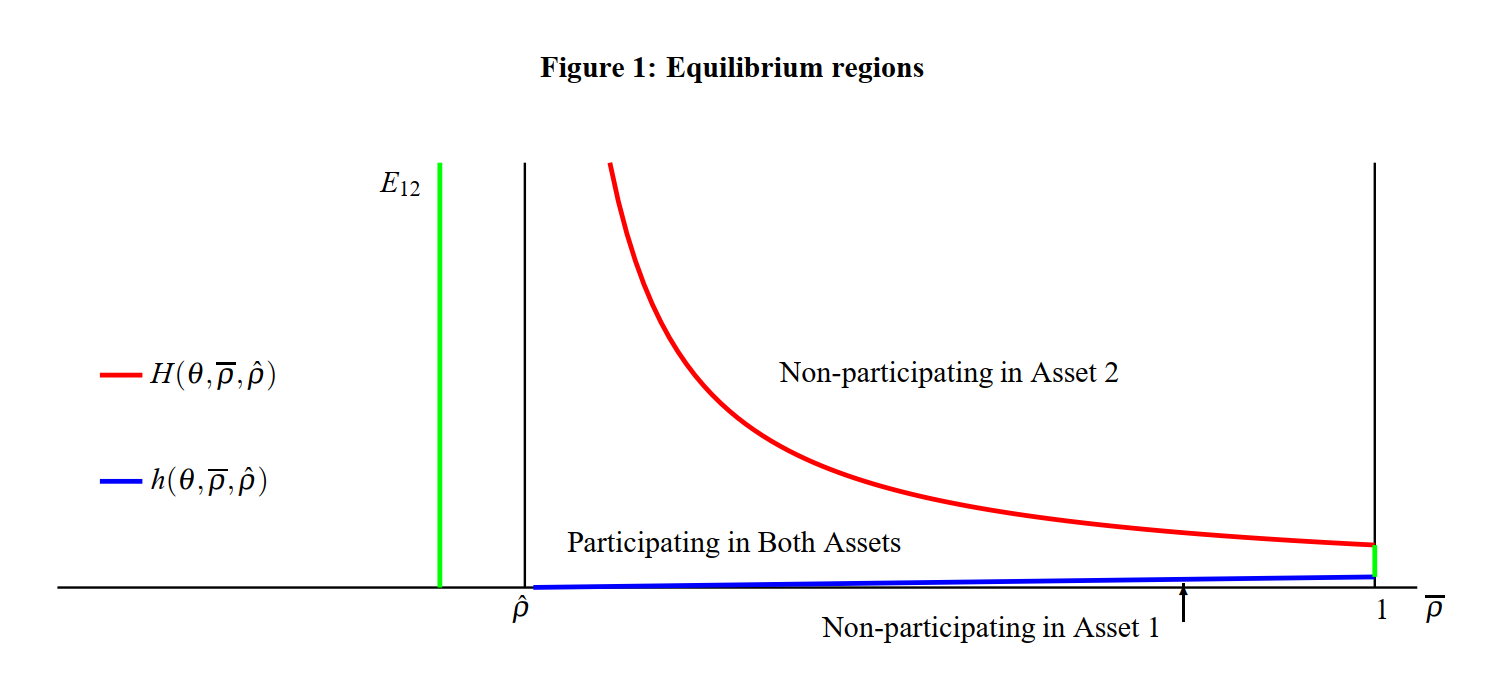
\includegraphics[width=1.0 \textwidth]{Figure1.png}
\end{figure}

%\newpage

\section{Implications for asset prices and market non-participation}
%\renewcommand{\theequation}{4.\arabic{equation}}
%\setcounter{equation}0

\quad \ 


在本节中,我们将深入研究均衡及其含义,并分析经济变化如何影响均衡类型和均衡价格。 我们对 CAPM 分析特别感兴趣,它显示了原始投资者比例的变化和最大相关系数的变化对资产价格的影响,这表明了不参与和``安全资产转移''现象的相互作用。

\subsection{CAPM analysis}
\quad \ 
为了阐明相关性暧昧和不参与的定价效应,我们现在转向风险资产的回报,看看它们是否具有偏离 CAPM 的超额回报 (alpha)。 对于资产 $i$,收益定义为:
\begin{equation*}
\tilde{Y}_i = \dfrac{\tilde{X}_i}{p_i} - 1, \qquad i = 1, 2,
\end{equation*}

市场回报(持有两种风险资产的全部供给)为:
\begin{equation*}
\tilde{Y}_M = \dfrac{\tilde{X}_1 Z_1^0 + \tilde{X}_2 Z_2^0}{p_1 Z_1^0 + p_2 Z_2^0} - 1. 
\end{equation*}



假设现在经济中存在的均衡是类型 1,即天真投资者不参与资产 1 的交易。那么从定理 2 可知均衡价格为:
\begin{eqnarray*}
p_1 = \mu_1 - \alpha \sigma_1 \left[ \dfrac{1 - \theta {\hat \rho}^2}{1 - \theta} \sigma_1 Z_1^0 + {\hat \rho} \sigma_2 Z_2^0 \right] \quad \text{and} \quad p_2 = \mu_2 - \alpha \sigma_2 \left[ {\hat \rho} \sigma_1 Z_1^0 + \sigma_2 Z_2^0 \right].
\end{eqnarray*}



现在假设在这个经济中有一个具有共同 CARA 效用函数的代表性投资者 (A)。 为了使均衡价格相同,代表性投资者必须持有以下信念:
\begin{equation*}
\mu_i^A = \mu_i, \quad \sigma_1^A = \sigma_1 \sqrt{\dfrac{1 - \theta \hat{\rho}^2}{1 - \theta}}, \quad \sigma_2^A = \sigma_2 \quad \text{and} \quad \rho^A = \hat{\rho} \sqrt{\dfrac{1 - \theta}{1 - \theta \hat{\rho}^2}}. 
\end{equation*}



代表性投资者对平均回报有正确的信念,因此他也会对平均收益有正确的信念:$ \tilde{Y}_i $ 代表资产 $i$ , $ \tilde{Y}_M $ 代表市场投资组合。 此外,从代表性投资者的角度来看,资产定价是正确的,CAPM 必须从他的角度来看。 即 \footnote{\baselineskip1.3em 由于我们将无风险资产的收益归一化为 0,$ \tilde{Y}_i $ 和 $ \tilde{Y}_M $ 的超额收益分别为 $ \overline{ Y}_i $ 和 $ \overline{Y}_M $。}
\begin{equation}
\overline{Y}_i = \beta_i^A \overline{Y}_M, \qquad i = 1, 2,
\end{equation}
其中 $ \beta_i^A $ 是资产 $i$ 对于代表性投资者而言的$\beta$值,由下式给出:
\begin{eqnarray*}
& \beta_1^A = \dfrac{Cov^A (\tilde{Y}_M, \tilde{Y}_1)}{Var^A (\tilde{Y}_M)} = \dfrac{p_1 Z_1^0 + p_2 Z_2^0}{p_1} \dfrac{\left[ \sigma_1^A \right]^2 Z_1^0 + \rho^A \sigma_1^A \sigma_2^A Z_2^0}{\left[ \sigma_1^A \right]^2 \left[ Z_1^0 \right]^2 + 2 \rho^A \sigma_1^A \sigma_2^A Z_1^0 Z_2^0 + \left[ \sigma_2^A \right]^2 \left[ Z_2^0 \right]^2}, & \\
& \beta_2^A = \dfrac{Cov^A (\tilde{Y}_M, \tilde{Y}_2)}{Var^A (\tilde{Y}_M)} = \dfrac{p_1 Z_1^0 + p_2 Z_2^0}{p_2} \dfrac{\rho^A \sigma_1^A \sigma_2^A Z_1^0 + \left[ \sigma_2^A \right]^2 Z_2^0}{\left[ \sigma_1^A \right]^2 \left[ Z_1^0 \right]^2 + 2 \rho^A \sigma_1^A \sigma_2^A Z_1^0 Z_2^0 + \left[ \sigma_2^A \right]^2 \left[ Z_2^0 \right]^2}. &
\end{eqnarray*}


注意到$ \rho^A \sigma_1^A = \hat{\rho} \sigma_1 $,所以上面的式可以用实际参数写成:
\begin{eqnarray*}
& \beta_1^A = \dfrac{Cov^A (\tilde{Y}_M, \tilde{Y}_1)}{Var^A (\tilde{Y}_M)} = \dfrac{p_1 Z_1^0 + p_2 Z_2^0}{p_1} \dfrac{\dfrac{1 - \theta \hat{\rho}^2}{1 - \theta} \sigma_1^2 Z_1^0 + \hat{\rho} \sigma_1 \sigma_2 Z_2^0}{\dfrac{1 - \theta \hat{\rho}^2}{1 - \theta} \sigma_1^2 \left[ Z_1^0 \right]^2 + 2 \hat{\rho} \sigma_1 \sigma_2 Z_1^0 Z_2^0 + \sigma_2^2 \left[ Z_2^0 \right]^2}, & \\
& \beta_2^A = \dfrac{Cov^A (\tilde{Y}_M, \tilde{Y}_2)}{Var^A (\tilde{Y}_M)} = \dfrac{p_1 Z_1^0 + p_2 Z_2^0}{p_2}
\dfrac{\hat{\rho} \sigma_1 \sigma_2 Z_1^0 + \sigma_2^2 Z_2^0}{\dfrac{1 - \theta \hat{\rho}^2}{1 - \theta} \sigma_1^2 \left[ Z_1^0 \right]^2 + 2 \hat{\rho} \sigma_1 \sigma_2 Z_1^0 Z_2^0 + \sigma_2^2 \left[ Z_2^0 \right]^2}. &
\end{eqnarray*}



在这个式中,市场收益与资产 $i$ 收益的协方差以及市场收益的方差是使用代表性投资者的人为信念而不是正确信念计算的。



代表性投资者对资产 1 的收益方差和相关系数的信念不正确,因为 $\sigma_1^A = \sigma_1 \sqrt{\dfrac{1 - \theta \hat{\rho}^2}{1 - \ theta}} $ 和 $ \rho^A = \hat{\rho} \sqrt{\dfrac{1 - \theta}{1 - \theta \hat{\rho}^2}} $,所以他对于市场的方差,市场收益与每种资产收益的协方差的信念是不正确的。因此,从代表性投资者的角度计算的 $\beta$ 值不是根据实际收益数据计算的 $\beta$ 。 现在考虑一位外部计量经济学家,他对整个经济有理性的信念,即他知道相关系数 $ \hat{\rho} $ 的真实值。 所以在他看来,
\begin{eqnarray*}
& \beta_1 = \dfrac{Cov (\tilde{Y}_M, \tilde{Y}_1)}{Var (\tilde{Y}_M)} = \dfrac{p_1 Z_1^0 + p_2 Z_2^0}{p_1} \dfrac{\sigma_1^2 Z_1^0 + \hat{\rho} \sigma_1 \sigma_2 Z_2^0}{\sigma_1^2 \left[ Z_1^0 \right]^2 + 2 \hat{\rho} \sigma_1 \sigma_2 Z_1^0 Z_2^0 + \sigma_2^2 \left[ Z_2^0 \right]^2}, & \\
& \beta_2 = \dfrac{Cov (\tilde{Y}_M, \tilde{Y}_2)}{Var (\tilde{Y}_M)} = \dfrac{p_1 Z_1^0 + p_2 Z_2^0}{p_2} \dfrac{\hat{\rho} \sigma_1 \sigma_2 Z_1^0 + \sigma_2^2 Z_2^0}{\sigma_1^2 \left[ Z_1^0 \right]^2 + 2 \hat{\rho} \sigma_1 \sigma_2 Z_1^0 Z_2^0 + \sigma_2^2 \left[ Z_2^0 \right]^2}, &
\end{eqnarray*}


其中方差和协方差是使用均衡收益的真实分布计算的。



两个实际的 $\beta$ 值都不同于代表性投资者的 $\beta$ 值,因此如果我们考虑实际经济中的 CAPM 模型,这两种资产的定价都是错误的。 这种定价错误可以在 $\alpha_i$ 中捕捉到,即市场调整后的回报:
\begin{equation*}
\alpha_i = \overline{Y}_i - \beta_i \overline{Y}_M = (\beta_i^A - \beta_i) \overline{Y}_M, \qquad i = 1, 2, 
\end{equation*}


其中第二个方程由(18)式可知。



为了确定$ \alpha_i $ 的符号,我们必须比较$ \beta_i^A $ 和$ \beta_i $。 观察 $\beta$ 的式,它们与函数 $ f (x) = \dfrac{a x + b}{c x + d} $ 具有相同的形式,其导数为:
\begin{equation*}
f^{\prime} (x) = \dfrac{a d - b c}{(c x + d)^2}.
\end{equation*}


$ f^{\prime} (x) > 0 $ 当且仅当 $ a d > b c $。 若令 $ a = \sigma_1^2 Z_1^0 $, $ b = \hat{\rho} \sigma_1 \sigma_2 Z_2^0 $, $ c = \sigma_1^2 \left[ Z_1^0 \right] ^2 $ , $ d = 2 \hat{\rho} \sigma_1 \sigma_2 Z_1^0 Z_2^0 + \sigma_2^2 \left[ Z_2^0 \right]^2 $,则 $ a d - b c = \hat {\rho} \sigma_1^3 \sigma_2 \left[ Z_1^0 \right]^2 Z_2^0 + \sigma_1^2 \sigma_2^2 Z_1^0 \left[ Z_2^0 \right]^2 = (\hat{\rho} \sigma_1 Z_1^0 + \sigma_2 Z_2^0) \sigma_1^2 \sigma_2 Z_1^0 Z_2^0 > 0 $。 注意到 $ \dfrac{1 - \theta\hat{\rho}^2}{1 - \theta} > 1 $,所以
\begin{equation*}
\alpha_1 = (\beta_1^A - \beta_1) \overline{Y}_M = \dfrac{p_1 Z_1^0 + p_2 Z_2^0}{p_1} \left[ f \left( \dfrac{1 - \theta\hat{\rho}^2}{1 - \theta} \right) - f (1) \right] \overline{Y}_M > 0,
\end{equation*} 

根据定理 2 的第一种情况,
\begin{equation*}
\overline{Y}_M = \dfrac{(\mu_1 - p_1) Z_1^0 + (\mu_2 - p_2) Z_2^0}{p_1 Z_1^0 + p_2 Z_2^0} = \alpha\dfrac{\dfrac{1 - \theta\hat{\rho}^2}{1 - \theta} \sigma_1^2 \left[ Z_1^0 \right]^2 + \hat{\rho} \sigma_1 \sigma_2 Z_1^0 Z_2^0 + \sigma_2^2 \left[ Z_2^0 \right]^2}{p_1 Z_1^0 + p_2 Z_2^0} > 0.
\end{equation*}



使用相同的方法,现在让 $ a = 0 $, $ b = \hat{\rho} \sigma_1 \sigma_2 Z_1^0 + \sigma_2^2 Z_2^0 $, $ c = \sigma_1^2 \left[ Z_1 ^0 \right]^2 $,$ d = 2 \hat{\rho} \sigma_1 \sigma_2 Z_1^0 Z_2^0 + \sigma_2^2 \left[ Z_2^0 \right]^2 $,则 $ a d - b c = - (\hat{\rho} \sigma_1 Z_1^0 + \sigma_2 Z_2^0) \sigma_1^2 \sigma_2 Z_1^0 Z_2^0 < 0 $。 
\begin{equation*}
\alpha_2 = (\beta_2^A - \beta_2) \overline{Y}_M = \dfrac{p_1 Z_1^0 + p_2 Z_2^0}{p_1} \left[ f \left( \dfrac{1 - \theta \hat{\rho}^2}{1 - \theta} \right) - f (1) \right] \overline{Y}_M < 0. 
\end{equation*}



通过均衡价格的对称性,我们得出结论,当天真投资者不参与资产 2 的交易时,$\alpha_2 > 0 $ 且 $\alpha_1 < 0 $。一般来说,不被天真投资者持有的资产存在正超额收益,被其持有其他风险资产的超额收益为负。 这是因为为了吸引精明投资者持有回报不明确的资产(根据天真投资者的说法),其价格必须足够低,即回报必须足够高。相反,暧昧厌恶的投资者会增持回报明确的资产,因而会提高其价格并降低其回报。



接下来,我们采用相同的方法来展示当均衡是参与均衡时相关系数暧昧的错误定价效应。当天真投资者交易两种风险资产时,均衡价格为:
\begin{eqnarray*}
& p_1 = \mu_1 - \alpha \sigma_1 \left[ Q (\theta, \overline{\rho}, {\hat \rho}) \sigma_1 Z_1^0 + q (\theta, \overline{\rho}, {\hat \rho}) \sigma_2 Z_2^0 \right] & \\
& p_2 = \mu_2 - \alpha \sigma_2 \left[ q (\theta, \overline{\rho}, {\hat \rho}) \sigma_1 Z_1^0 + Q (\theta, \overline{\rho}, {\hat \rho}) \sigma_2 Z_2^0 \right]. &
\end{eqnarray*}



为了使代表性投资者 (A) 的经济具有相同的均衡价格,代理人必须相信 $ \mu_i^A = \mu_i $, $ \left[ \sigma_i^A \right]^2 = \sigma_i^ 2 Q (\theta, \overline{\rho}, {\hat \rho}) $ 和 $ \rho^A = \dfrac{q (\theta, \overline{\rho}, {\hat \rho}) }{Q (\theta, \overline{\rho}, {\hat \rho})} $.
%\begin{eqnarray*}
%& \left[ \sigma_i^A \right]^2 = \sigma_i^2 Q (\theta, \overline{\rho}, {\hat \rho}) & \\
%& \rho^A = \dfrac{q (\theta, \overline{\rho}, {\hat \rho})}{Q (\theta, \overline{\rho}, {\hat \rho})}. &
%\end{eqnarray*}


根据代表性投资者,两种风险资产的 $\beta$ 根据实际参数写为:
\begin{equation*}
\beta_1^A = \dfrac{p_1 Z_1^0 + p_2 Z_2^0}{p_1} \dfrac{\sigma_1^2 Z_1^0 + \rho^A \sigma_1 \sigma_2 Z_2^0}{\sigma_1^2 \left[ Z_1^0 \right]^2 + 2 \rho^A \sigma_1 \sigma_2 Z_1^0 Z_2^0 + \sigma_2^2 \left[ Z_2^0 \right]^2}, 
\end{equation*}
\begin{equation*}
\beta_2^A = \dfrac{p_1 Z_1^0 + p_2 Z_2^0}{p_2} \dfrac{\rho^A \sigma_1 \sigma_2 Z_1^0 + \sigma_2^2 Z_2^0}{\sigma_1^2 \left[ Z_1^0 \right]^2 + 2 \rho^A \sigma_1 \sigma_2 Z_1^0 Z_2^0 + \sigma_2^2 \left[ Z_2^0 \right]^2}. 
\end{equation*}


因此,$ \alpha_i $ 由下式给出:

\begin{equation*}
\alpha_i = \overline{Y}_i - \beta_i \overline{Y}_{M} = (\beta_i^A - \beta_i) \overline{Y}_M, \qquad i = 1, 2.
\end{equation*}



对于函数 $ f (x) = \dfrac{a x + b}{c x + d} $,取参数  $ a = \sigma_1 \sigma_2 Z_2^0 $,$ b = \sigma_1^2 Z_1^0 $,$ c = 2 \sigma_1 \sigma_2 Z_1^0 Z_2^0 $ ,$ d = \sigma_1^2 \left[ Z_1^0 \right]^2 + \sigma_2^2 \left[ Z_2^0 \right]^2 $。 由于 $ a d - b c = \left( \sigma_2^2 \left[ Z_2^0 \right]^2 - \sigma_1^2 \left[ Z_1^0 \right]^2 \right) \sigma_1 \sigma_2 Z_2^0 $,  $ f (\cdot) $ 是一个递增函数当且仅当 $ \sigma_1 Z_1^0 < \sigma_2 Z_2^0 $。 由于

\begin{equation*}
\overline{Y}_M = Q (\theta, \overline{\rho}, {\hat \rho}) \dfrac{\alpha \left[ \left[ Z_1^0 \right]^2 + \rho^A \sigma_1 \sigma_2 Z_1^0 Z_2^0 + \sigma_2^2 \left[ Z_2^0 \right]^2 \right]}{p_1 Z_1^0 + p_2 Z_2^0} > 0, 
\end{equation*}


 以及$ \rho^A > \hat{\rho} $,我们有
\begin{equation*}
\alpha_1 = (\beta_1^A - \beta_1) \overline{Y}_M = \dfrac{p_1 Z_1^0 + p_2 Z_2^0}{p_1} \left[ f (\rho^A) - f (\hat{\rho}) \right]\overline{Y}_M > 0,
\end{equation*}


当且仅当 $ \sigma_1 Z_1^0 < \sigma_2 Z_2^0 $; 由对称性可知$ \alpha_2 < 0 $。 类似地,如果 $ \sigma_1 Z_1^0 > \sigma_2 Z_2^0 $ 那么 $ \alpha_1 < 0 $ 且 $ \alpha_2 > 0 $。





注意到,在非参与均衡下,天真投资者将不持有质量较低的资产。因此,概括起来,在三种均衡下,质量较低的资产将产生正超额收益,而质量较高的资产将产生负超额收益。也就是说,无论经济处于参与均衡还是非参与均衡,天真投资者都会偏爱质量更高的资产,甚至达到非理性的程度,使其价格上涨, 从而回报低于标准模型的预测。 由此我们可以看出,相关性暧昧拓展了股票横截面研究的新思路。

上述分析总结在命题 4 中。
\begin{prop}
无论均衡是否为参与均衡,质量较低的风险资产将产生正超额收益,而质量较高的资产将产生负超额收益。
\end{prop}

\subsection{天真投资者的比例}

\quad \ 


现在我们通过分析均衡类型是否改变以及均衡价格如何随着 $ \theta $ 的变化而变化,来展示天真投资者的比例如何影响均衡结果。通过对称性,我们只展示对类型 [1] 均衡的分析, 并且将立即实现类型 [3] 均衡的类似结果。



首先,我们假设当 $ \theta $ 足够小时,经济处于类型 [1] 均衡。 此时风险资产的均衡价格为:
\begin{eqnarray*}
& p_1 = \mu_1 - \alpha \sigma_1 \left\{ \dfrac{1 - {\hat \rho}^2}{1 - \theta} \sigma_1 Z_1^0 + {\hat \rho} \left[ {\hat \rho} \sigma_1 Z_1^0 + \sigma_2 Z_2^0 \right] \right\} & \\
& p_2 = \mu_2 - \alpha \sigma_2 \left[ {\hat \rho} \sigma_1 Z_1^0 + \sigma_2 Z_2^0 \right] &
\end{eqnarray*}


这一情形要求资产 1 的质量与资产 2 相比足够小,即$ E_{1 2} \leqslant h (\theta, \overline{\rho}, {\hat \rho}) $。 $ p_2 $ 不受 $ \theta $ 影响,而 $ p_1 $ 是 $ \theta $ 的减函数,如果 $ \theta $ 趋近于 1 ,则$p_1$趋近于负无穷。因此,如果 $ \theta $ 增加到一定值,均衡类型将转变为参与型。计算表明偏移的临界值为 $ \theta_1 = 1 - \dfrac{1 - {\hat \rho}^2}{\overline{\rho} - {\hat \rho}} \dfrac{1 }{{\hat \rho} + E_{2 1}} < 1 $。 $ \theta_1 > 0 $ 等价于 $ E_{1 2} < \dfrac{\overline{\rho} - {\hat \rho}}{1 - \overline{\rho} {\hat \rho}} $,这是显而易见的,因为 $ h (\theta, \overline{\rho}, {\hat \rho}) < \dfrac{\overline{\rho} - {\hat \rho}}{1 - {\hat \ rho} \overline{\rho}} $。因此 $ 0 < \theta_1 < 1 $。因此,如果能出现类型[1]的均衡,$\theta_1\in(0, 1)$,这与其经济意义是一致的。当$ \theta > \theta_1 $ 时,参与均衡出现,此时$ h (\theta, \overline{\rho}, {\hat \rho}) < E_{1 2} < H (\theta, \overline{\rho}, {\hat \rho}) $。由于 $ h (\theta, \overline{\rho}, {\hat \rho}) $ 关于 $ \theta $ 递减和 $ H (\theta, \overline{\rho}, {\hat \rho}) = \dfrac{1}{h (\theta, \overline{\rho}, {\hat \rho})} $ 关于$\theta$递增,因此当 $ \theta $ 继续增加时,均衡类型保持不变。



其次,假设当 $ \theta $ 足够小时,经济处于类型 [3] 均衡。 那么风险资产的均衡价格为:

\begin{eqnarray*}
& p_1 = \mu_1 - \alpha \sigma_1 \left[ \sigma_1 Z_1^0 + {\hat \rho} \sigma_2 Z_2^0 \right] & \\
& p_2 = \mu_2 - \alpha \sigma_2 \left\{ \dfrac{1 - {\hat \rho}^2}{1 - \theta} \sigma_2 Z_2^0 + {\hat \rho} \left[ \sigma_1 Z_1^0 + {\hat \rho} \sigma_2 Z_2^0 \right] \right\} &
\end{eqnarray*}


这一情形要求资产 1 的质量与资产 2 相比足够大,$H (\theta, \overline{\rho}, {\hat \rho}) \leqslant E_{1 2} $。 $ p_1 $ 不受$ \theta $ 的影响,而 $ p_2 $ 是$ \theta $ 的递减函数,若$ \theta $ 趋近于1,则 $ p_2 $ 趋近于负无穷。因此,如果$ \theta $ 增加到某个值,则均衡类型将转变为参与均衡类型。我们可以计算出偏移的临界值为 $ \theta_2 = 1 - \dfrac{1 - {\hat \rho}^2}{\overline{\rho} - {\hat \rho}} \dfrac{1 }{E_{1 2} + {\hat \rho}} < 1 $。 $ \theta_2 > 0 $ 等价于 $ E_{1 2} > \dfrac{1 - \overline{\rho} {\hat \rho}}{\overline{\rho} - {\hat \rho}} $,这是显而易见的,因为 $ \dfrac{1 - \overline{\rho} {\hat \rho}}{\overline{\rho} - {\hat \rho}} < H (\theta, \overline{\rho }, {\hat \rho}) $。因此 $ 0 < \theta_2 < 1 $。因此,如果能出现类型[3]的均衡,$\theta_2\in(0, 1)$,这与其经济意义是一致的。当$ \theta > \theta_2 $ 时,参与均衡出现,此时$ h (\theta, \overline{\rho}, {\hat \rho}) < E_{1 2} < H (\theta, \overline{\rho}, {\hat \rho}) $。由于$ H (\theta, \overline{\rho}, {\hat \rho}) $ 关于$ \theta $ 递增,因此当$ \theta $ 继续减少时,均衡将保持相同类型。




在上述分析中,我们首先假设当 $ \theta $ 足够小时经济处于非参与均衡, $ \dfrac{\overline{\rho} - {\hat \rho}}{1 - {\hat \rho} \overline{\rho}} < E_{1 2} \leqslant 1 $的情形不可能出现,因为在这种情况下 $\theta_{1}$ 将是负数。 因此,如果 $ \dfrac{\overline{\rho} - {\hat \rho}}{1 - {\hat \rho} \overline{\rho}} < E_{1 2} \leqslant 1 $,则经济中发生的只能是参与均衡,因此此时$ \theta $ 的变化不能改变均衡的类型。 同样,当 $ 1 \leqslant E_{1 2} < \dfrac{1 - {\hat \rho} \overline{\rho}}{\overline{\rho} - {\hat \rho}} $,不管 $ \theta $ 有多小,均衡不可能是类型[3]。 我们在命题 5 中总结了我们的分析。

\vskip 8 pt

\begin{prop}


当 $ \dfrac{\overline{\rho} - {\hat \rho}}{1 - {\hat \rho} \overline{\rho}} < E_{1 2} < \dfrac{1 - {\hat \rho} \overline{\rho}}{\overline{\rho} - {\hat \rho}} $,均衡只能是参与均衡,$ \theta $ 的变化不会改变均衡类型。 但是如果$ E_{1 2} $ 不在区间内,增加$ \theta $ 可能会使均衡类型从非参与型转变为参与型。
\end{prop}

\vskip 8 pt


直觉上,人们可能会认为随着天真投资者比例的增加,均衡价格将单调增加,因为天真投资者通常被认为比精明投资者更保守。 然而,如第 2 节所述,我们发现天真投资者可能比精明投资者持有更激进的头寸,因此增加 $\theta $ 可能会增加对资产的需求并降低均衡价格。因此,当 $ \theta $ 从 0 到 1 变化时,均衡价格变化可能是非单调的。我们在命题 6 中展示了这一结果:

\vskip 8 pt

\begin{prop}



如果 $ E_{1 2} < 1 $,则资产 1 的均衡价格关于 $ \theta $ 递减,如果 $ E_{1 2} > \dfrac{1 - {\hat \rho} \overline{\rho}}{\overline{\rho} - {\hat \rho}} $,资产 1 的均衡价格关于 $ \theta $ 先升后降。
如果 $ E_{2 1} < 1 $,则资产 2 的均衡价格关于 $ \theta $ 递减,如果 $ E_{2 1} > \dfrac{1 - {\hat \rho} \overline{\rho}}{\overline{\rho} - {\hat \rho}} $,资产 2 的均衡价格关于 $ \theta $ 先升后降。
\end{prop}

\subsection{Maximum correlation coefficient}

\quad \ 


正如我们在第 3 节中指出的那样,在均衡状态下,只有天真投资者的先验集合 $ [\underline{\rho}, \overline{\rho}] $ 的最大相关系数 $ \overline{\rho} $ 会影响到他们的有限参与决定和资产价格,因此 $ \Delta \rho = \overline{\rho} - \hat{\rho} $ 可以被视为他们所面临的暧昧程度的衡量指标。$\Delta \rho $ 是由投资者的经验、知识或信心以及市场环境共同决定的。接下来我们研究最大相关系数(暧昧性水平)的变化如何影响均衡类型和资产价格。



固定其他参数不变,增加$ \overline{\rho} $ 可以改变均衡类型并且可以观察到“安全资产转移”现象。请注意,当且仅当 $ h (\theta, \overline{\rho}, {\hat \rho}) < E_{12} < H (\theta, \overline{\rho}, {\hat \rho})$时,参与均衡才会出现。当 $ \overline{\rho} $ 从 $ \hat{\rho} $ 变化到 $1$ 时,$ h (\theta, \overline{\rho}, {\hat \rho}) $ 从 $0$ 增加到 $ \dfrac{1 - \theta}{1 + \theta \hat{\rho}} < 1 $, $ H (\theta, \overline{\rho}, {\hat \rho}) $ 从无穷大减小到$ \dfrac{1 + \theta \hat{\rho}}{1 - \theta} > 1 $。因此,如果质量比率 $ E_{12} $ 满足 $ \dfrac{1 - \theta}{1 + \theta\hat{\rho}} \leqslant E_{12} \leqslant \dfrac{1 + \theta\ hat{\rho}}{1 - \theta} $,均衡必然是参与均衡。如果 $ E_{12} < \dfrac{1 - \theta}{1 + \theta \hat{\rho}} $(或 $ E_{12} > \dfrac{1 + \theta \hat{\rho} }{1 - \theta} $),增加最大相关系数可以改变 $ E_{12} $ 和 $ h (\theta, \overline{\rho}, {\hat \rho}) $ (或者 $H (\theta, \overline{\rho}, {\hat \rho}) $),从而将均衡从参与均衡切换到非参与均衡,此时天真投资者只会交易更高质量的资产。



我们也可以直观地理解这一点。请注意,要持有这两种资产,天真投资者必须容忍相关系数的暧昧性。当质量比率足够小或足够大时,这两种资产有着明显的区别。随着市场对它们变得更加不确定,$ \overline{\rho} $ 不断增大,为了避免暧昧性,天真投资者将选择只持有质量更高的资产,导致非参与均衡。这一结果总结在命题 7 中。

\vskip 8 pt

\begin{prop}


当 $ \dfrac{1 - \theta}{1 + \theta \hat{\rho}} \leqslant E_{12} \leqslant \dfrac{1 + \theta \hat{\rho}}{1 - \theta} $时,$ \overline{\rho} $ 的变化不会改变均衡类型,均衡只能是参与的。 但是,如果 $ E_{1 2} $ 不在该区间内, $ \overline{\rho} $ 的增大可能会将均衡类型从参与型转变为非参与型,并且天真投资者将持有更高质量的资产。
\end{prop}



命题 5、6 和 7 表明,如果经济处于非参与均衡,并且我们希望通过提高天真投资者的比例或减小最大相关系数来增加市场参与,那么其他资产的非参与不会发生。因为在均衡状态下,更高质量的资产将始终由天真投资者持有。

\vskip 8 pt



根据我们的分析,减小最大相关系数将提高市场参与度。如 Caballero 和 Krishnamurthy(2007)以及 Easley 和 O'Hara(2009)所示,一个包含天真投资者的经济体需要一些机制(如最后贷款人、存款保险)和法规(如非上市证券披露、适用性规则)以减小天真投资者的最大相关系数,从而帮助他们更客观的做出更好的决策。我们的分析也支持这些观点。以关联交易的监管为例。\footnote{\baselineskip1.3em FASB 和 SEC 都制定了规范关联交易披露的规则。例如,FASB 在 FAS 57 中描述了关联交易的披露要求。} 复杂的关联交易会以一种微妙的方式影响关联方的财务报表(Kohlbeck 和 Mayhew,2004),但披露要求和其他相关规则将有助于减小他们之间相关系数的暧昧性,因此对于天真投资者来说,相关系数的暧昧程度降低。



至于均衡价格,定理 2 表明,如果经济处于非参与均衡,则 $ \overline{\rho} $ 的变化对资产价格没有影响,因为天真投资者只交易一种风险资产。至于在参与均衡中$ \overline{\rho} $ 的变化如何影响资产价格,见命题 8。

\begin{prop}


在参与均衡下,当 $ E_{1 2} \geqslant \dfrac{2 (1 - \theta) (1 + \theta \hat{\rho})}{(1 - \theta)^2 + (1 + \theta\hat{\rho})^2} $时, $ p_1 $ 是 $ \overline{\rho} $ 的减函数。 当 $ E_{1 2} < \dfrac{2 (1 - \theta) (1 + \theta \hat{\rho})}{(1 - \theta)^2 + (1 + \theta\hat{ \rho})^2} $时, $ p_1 $ 随 $ \overline{\rho} $ 从 $ \hat{\rho} $ 变为 $1$ 先减小后增大。 至于资产 2 价格 $ p_2 $ ,结论是对称的。

\end{prop}



因此,尽管减小$ \overline{\rho} $ 的政策可以有效地提高一种资产(质量较低)的市场参与,但它可能会对另一种资产的价格产生一些负面影响。 因此在这种情况下,如何衡量相关政策的总社会效应变得至关重要。\footnote{\baselineskip1.3em Easley, O'Hara, 和 Yang (2014) 讨论了暧昧性给社会福利带来的影响。在他们的模型中,福利函数是透明交易者的事前均衡效用的确定性等价。 他们发现降低暧昧性不一定会使福利函数增加。}我们的结果表明,对政策的评估应该考虑到暧昧性,并且在评估这些政策的影响时需要仔细校准。

\section{Conclusions}
\renewcommand{\theequation}{5.\arabic{equation}}
\setcounter{equation}0

\quad \ 

在本文中,我们研究了相关系数暧昧性在金融市场中的作用。特别地,我们通过假设经济中一部分投资者认为风险资产的相关系数是暧昧的,由此扩展了 Easley 和 O'Hara (2009) 的多资产模型。巧妙地定义夏普比率 [类似于Sharpe(1966)] 会带来技术上的便利。相关性的暧昧性在需求函数中产生了四种情景,从而使需求曲线连续但存在结点。在特定条件下,理性的暧昧厌恶的天真投资者选择有限参与,以避免相关性系数暧昧性。天真投资者与精明投资者以相同的方向交易两种风险资产,但他们不一定会持有更保守的立场。



需求函数的性质导致三种不同类型的均衡。我们在 $ \overline{\rho} - O - E_{12} $ 平面中展示了均衡区域。标准差和人均禀赋的乘积$ \sigma_i Z_i^0 $ 衡量了资产$i$ 的质量。当质量比率足够小或足够大时,较低质量资产的有限参与作为一种内生的结果出现。 CAPM 分析表明,较低质量的资产总是会产生正的超额收益。均衡的比较静态分析表明,天真投资者的比例或最大相关系数的变化会影响市场参与,同时如果均衡从参与型转变为非参与型,则可以观察到“安全资产转移”现象。然而,这两个参数变化的定价效应是非单调的,表明相关政策产生了深远的社会影响。



我们的模型可以扩展到两个方向。一个扩展是我们可以以类似于 Cao, Wang 和 Zhang (2005) 的方式进一步考虑暧昧厌恶投资者之间异质性的影响,以便进一步了解不同程度的暧昧性将如何影响投资决策。另一个自然扩展是考虑在动态环境中学习相关性系数暧昧性。有大量关于相关结构时变特征的文献,例如 Bollerslev, Engle 和 Wooldridge (1988) 提出的关于协方差矩阵的 GARCH 过程,以及 Aydemir (2008) 构建的逆周期模式。因此,如果我们考虑一个模型,其中投资人将相关性视为具有暧昧性的随机过程,那么我们可以研究相关系数暧昧下的金融市场动态。

%\newpage



\section*{Appendix}
\renewcommand{\theequation}{A.\arabic{equation}}
\setcounter{equation}0

\subsection*{A.1 \quad Proof of Theorem 1}

\quad \ 

为了求原规划(9)的最优解,我们需要考虑以下四个问题:

\begin{enumerate}
\item $ \max\limits_{z_1 z_2 < 0} \min\limits_{\rho \in [\underline{\rho}, \overline{\rho}]} f (z_1, z_2, \rho) = \max\limits_{z_1 z_2 < 0} f (z_1, z_2, \underline{\rho}) $,
\item $ \max\limits_{z_1 z_2 > 0} \min\limits_{\rho \in [\underline{\rho}, \overline{\rho}]} f (z_1, z_2, \rho) = \max\limits_{z_1 z_2 > 0} f (z_1, z_2, \overline{\rho}) $,
\item $ \max\limits_{z_1 = 0} \min\limits_{\rho \in [\underline{\rho}, \overline{\rho}]} f (z_1, z_2, \rho) = \max\limits_{z_2} f (0, z_2, \rho) $,
\item $ \max\limits_{z_2 = 0} \min\limits_{\rho \in [\underline{\rho}, \overline{\rho}]} f (z_1, z_2, \rho) = \max\limits_{z_1} f (z_1, 0, \rho) $,
\end{enumerate}

然后尝试找到对应于原始问题(9)的最优解的最大值。

我们首先考虑问题1: $ \max\limits_{z_1 z_2 < 0} \min\limits_{\rho \in [\underline{\rho}, \overline{\rho}]} f (z_1, z_2, \rho) = \max\limits_{z_1 z_2 < 0} f (z_1, z_2, \underline{\rho}) $, 其中

\begin{eqnarray*}
f (z_1, z_2, \underline{\rho}) = \sigma_1 R_1 z_1 + \sigma_2 R_2 z_2 - \frac12 \alpha [\sigma_1^2 z_1^2 + 2 \underline{\rho} \sigma_1 \sigma_2 z_1 z_2 + \sigma_2^2 z_2^2] + w.
\end{eqnarray*}

计算表明,天真投资者对风险资产的需求函数为:
\begin{eqnarray}
Z_N^* = \left( \begin{matrix} Z_{N 1}^* \\ Z_{N 2}^* \end{matrix} \right) = \dfrac1{\alpha (1 - \underline{\rho}^2)} \left( \begin{matrix} \dfrac{R_1 - \underline{\rho} R_2}{\sigma_1} \\ \dfrac{R_2 - \underline{\rho} R_1}{\sigma_2} \end{matrix} \right)
\end{eqnarray}
如果 $ Z_{N 1}^* Z_{N 2}^* < 0 $,即 $ (R_1 - \underline{\rho} R_2) (R_2 - \underline{\rho} R_1) < 0 $, 等价地,我们有
\begin{eqnarray}
(N1.1) \quad \left\{ \begin{matrix} R_1 < \underline{\rho} R_2 \\ R_2 > \underline{\rho} R_1 \end{matrix} \right. \qquad \text{或} \qquad (N1.2) \quad \left\{ \begin{matrix} R_1 > \underline{\rho} R_2 \\ R_2 < \underline{\rho} R_1 \end{matrix} \right..
\end{eqnarray}
因此
\begin{eqnarray*}
\max\limits_{z_1 z_2 < 0} \min\limits_{\rho \in [\underline{\rho}, \overline{\rho}]} f (z_1, z_2, \rho) = f (Z_{N 1}^*, Z_{N 2}^*, \underline{\rho}) = \dfrac{R_1^2 - 2 \underline{\rho} R_1 R_2 + R_2^2}{2 \alpha (1 - \underline{\rho}^2)} + w.
\end{eqnarray*}
然后我们考虑问题 2:$ \max\limits_{z_1 z_2 > 0} \min\limits_{\rho \in [\underline{\rho}, \overline{\rho}]} f (z_1, z_2, \rho) = \max\limits_{z_1 z_2 > 0} f (z_1, z_2, \overline{\rho}) $,其中
\begin{eqnarray*}
f (z_1, z_2, \overline{\rho}) = \sigma_1 R_1 z_1 + \sigma_2 R_2 z_2 - \frac12 \alpha [\sigma_1^2 z_1^2 + 2 \overline{\rho} \sigma_1 \sigma_2 z_1 z_2 + \sigma_2^2 z_2^2] + w.
\end{eqnarray*}
计算表明,天真投资者对风险资产的需求函数为:
\begin{eqnarray}
Z_N^* = \left( \begin{matrix} Z_{N 1}^* \\ Z_{N 2}^* \end{matrix} \right) = \dfrac1{\alpha (1 - \overline{\rho}^2)} \left( \begin{matrix} \dfrac{R_1 - \overline{\rho} R_2}{\sigma_1} \\ \dfrac{R_2 - \overline{\rho} R_1}{\sigma_2} \end{matrix} \right)
\end{eqnarray}
如果 $ Z_{N 1}^* Z_{N 2}^* > 0 $, 即 $ (R_1 - \overline{\rho} R_2) (R_2 - \overline{\rho} R_1) > 0 $, 等价地,我们有
\begin{eqnarray}
(N2.1) \quad \left\{ \begin{matrix} R_1 < \overline{\rho} R_2 \\ R_2 < \overline{\rho} R_1 \end{matrix} \right. \qquad \text{或} \qquad (N2.2) \quad \left\{ \begin{matrix} R_1 > \overline{\rho} R_2 \\ R_2 > \overline{\rho} R_1 \end{matrix} \right.
\end{eqnarray}
因此
\begin{eqnarray*}
\max\limits_{z_1 z_2 > 0} \min\limits_{\rho \in [\underline{\rho}, \overline{\rho}]} f (z_1, z_2, \rho) = f (Z_{N 1}^*, Z_{N 2}^*, \overline{\rho}) = \dfrac{R_1^2 - 2 \overline{\rho} R_1 R_2 + R_2^2}{2 \alpha (1 - \overline{\rho}^2)} + w
\end{eqnarray*}

我们接下来考虑问题 3: $ \max\limits_{z_1 = 0} \min\limits_{\rho \in [\underline{\rho}, \overline{\rho}]} f (z_1, z_2, \rho) = \max\limits_{z_2} f (0, z_2, \rho) $。
二次曲面 $ f (z_1, z_2, \rho) $ 在平面 $ z_1 = 0 $ 处截取抛物线 1:
\begin{eqnarray*}
f (0, z_2, \rho) = \sigma_2 R_2 z_2 - \frac12 \alpha \sigma_2^2 z_2^2 + w \qquad \text{和} \qquad z_1 = 0
\end{eqnarray*}
抛物线 1 的顶点是 $ \left( 0, \dfrac{R_2}{\alpha \sigma_2} \right) $,
\begin{eqnarray}
Z_N^* = \left( \begin{matrix} Z_{N 1}^* \\ Z_{N 2}^* \end{matrix} \right) = \dfrac1{\alpha} \left( \begin{matrix} 0 \\ \dfrac{R_2}{\sigma_2} \end{matrix} \right)
\end{eqnarray}
和 $ \max\limits_{z_2} f (0, z_2, \rho) = f \left( 0, \dfrac{R_2}{\alpha \sigma_2}, \rho \right) = \dfrac{R_2^2} {2 \alpha} + w $。

最后,我们考虑问题4: $ \max\limits_{z_2 = 0} \min\limits_{\rho \in [\underline{\rho}, \overline{\rho}]} f (z_1, z_2, \rho ) = \max\limits_{z_1} f (z_1, 0, \rho) $。
二次曲面 $ f (z_1, z_2, \rho) $ 在平面 $ z_2 = 0 $ 处截取抛物线 2:

\begin{eqnarray*}
f (z_1, 0, \rho) = \sigma_1 R_1 z_1 - \frac12 \alpha \sigma_1^2 z_1^2 + w \qquad \text{and} \qquad z_2 = 0.
\end{eqnarray*}
抛物线 2 的顶点是 $ \left( \dfrac{R_1}{\alpha \sigma_1}, 0 \right) $,并 $ \max\limits_{z_1} f (z_1, 0, \rho) = f \left( \dfrac{R_1}{\alpha \sigma_1}, 0, \rho \right) =\dfrac{R_1^2} {2 \alpha} + w $。
\begin{eqnarray}
Z_N^* = \left( \begin{matrix} Z_{N 1}^* \\ Z_{N 2}^* \end{matrix} \right) = \dfrac1{\alpha} \left( \begin{matrix} \dfrac{R_1}{\sigma_1} \\ 0 \end{matrix} \right)
\end{eqnarray}

条件 (A.2) $ (R_1 - \underline{\rho} R_2) (R_2 - \underline{\rho} R_1) < 0 $ 与条件 (A.4) $ (R_1 - \overline{ \rho} R_2) (R_2 - \overline{\rho} R_1) > 0 $ 不可能同时成立。也就是说在平面 $ R_1 - O - R_2 $上
\begin{eqnarray*}
\{ (R_1, R_2) | (R_1 - \underline{\rho} R_2) (R_2 - \underline{\rho} R_1) < 0 \} \cap \{ (R_1, R_2) | (R_1 - \overline{\rho} R_2) (R_2 - \overline{\rho} R_1) > 0 \} = \emptyset
\end{eqnarray*}
成立。因此,我们将规划 3 和 4 的可行域视为条件 (A.2) 和 (A.4) 的两个补集的交集:

\begin{eqnarray*}
D & = & \{ (R_1, R_2) | (R_1 - \underline{\rho} R_2) (R_2 - \underline{\rho} R_1) < 0 \}^c \cap \{ (R_1, R_2) | (R_1 - \overline{\rho} R_2) (R_2 - \overline{\rho} R_1) > 0 \}^c \\
& = & \left[ \{ (R_1, R_2) | (R_1 - \underline{\rho} R_2) (R_2 - \underline{\rho} R_1) < 0 \} \cup \{ (R_1, R_2) | (R_1 - \overline{\rho} R_2) (R_2 - \overline{\rho} R_1) > 0 \} \right]^c \\
& = & \{ (R_1, R_2) | (R_1 - \underline{\rho} R_2) (R_2 - \underline{\rho} R_1) \geqslant 0 \} \cap \{ (R_1, R_2) | (R_1 - \overline{\rho} R_2) (R_2 - \overline{\rho} R_1) \leqslant 0 \}.
\end{eqnarray*}


我们通过两种方法分析这个交集。 对于以下三种情况,我们首先考虑 $R_1$ 的符号。


情形 1.1:$ R_1 < 0 $,则 $ R_2 - \underline{\rho} R_1 < R_2 - \overline{\rho} R_1 $。

(1.1.1) 如果 $ R_2 - \underline{\rho} R_1 < R_2 - \overline{\rho} R_1 < 0 $,则 $ R_1 - \underline{\rho} R_2 \leqslant 0 \leqslant R_1 - \overline {\rho} R_2 $,因此 $ R_2 < 0 $ 且 $ \overline{\rho} R_2 \leqslant R_1 \leqslant \underline{\rho} R_2 $。

(1.1.2) 如果 $ R_2 - \underline{\rho} R_1 < R_2 - \overline{\rho} R_1 = 0 $,则 $ R_1 - \underline{\rho} R_2 \leqslant 0 $,因此 $ R_2 = \overline{\rho} R_1 $ 且 $ R_1 \leqslant \underline{\rho} R_2 $。

(1.1.3) 如果 $ R_2 - \underline{\rho} R_1 < 0 < R_2 - \overline{\rho} R_1 $,则 $ R_1 - \underline{\rho} R_2 \leqslant 0 $ 且 $ R_1 - \overline{\rho} R_2 \leqslant 0 $,因此 $ \overline{\rho} R_1 < R_2 < \underline{\rho} R_1 $。

(1.1.4) 如果 $ 0 = R_2 - \underline{\rho} R_1 < R_2 - \overline{\rho} R_1 $,则 $ R_1 - \overline{\rho} R_2 \leqslant 0 $,因此 $ R_2 = \underline{\rho} R_1 $ 且 $ R_1 \leqslant \overline{\rho} R_2 $。

(1.1.5) 如果 $ 0 < R_2 - \underline{\rho} R_1 < R_2 - \overline{\rho} R_1 $,则 $ R_1 - \overline{\rho} R_2 \leqslant 0 \leqslant R_1 - \underline {\rho} R_2 $,因此 $ R_2 > 0 $ 且 $ \underline{\rho} R_2 \leqslant R_1 \leqslant \overline{\rho} R_2 $。

情形 1.2:$ R_1 = 0 $,则 $ - \underline{\rho} R_2^2 \geqslant 0 $ 且 $ - \overline{\rho} R_2^2 \leqslant 0 $,因此 $ R_2 = 0 $ 或 $ \underline{\rho} \leqslant 0 \leqslant \overline{\rho} $。

情形 1.3:$ R_1 > 0 $,则 $ R_2 - \overline{\rho} R_1 < R_2 - \underline{\rho} R_1 $。

(1.3.1) 如果 $ R_2 - \overline{\rho} R_1 < R_2 - \underline{\rho} R_1 < 0 $,则 $ R_1 - \underline{\rho} R_2 \leqslant 0 \leqslant R_1 - \overline {\rho} R_2 $,因此 $ R_2 < 0 $ 且 $ \overline{\rho} R_2 \leqslant R_1 \leqslant \underline{\rho} R_2 $。

(1.3.2) 如果 $ R_2 - \overline{\rho} R_1 < R_2 - \underline{\rho} R_1 = 0 $,则 $ 0 \leqslant R_1 - \overline{\rho} R_2 $,因此 $ R_2 = \underline{\rho} R_1 $ 且 $ \underline{\rho} R_2 \leqslant R_1 $。

(1.3.3) 如果 $ R_2 - \overline{\rho} R_1 < 0 < R_2 - \underline{\rho} R_1 $,则 $ 0 \leqslant R_1 - \underline{\rho} R_2 $ 且 $ 0 \leqslant R_1 - \overline{\rho} R_2 $,因此 $ \underline{\rho} R_1 < R_2 < \overline{\rho} R_1 $。

(1.3.4) 如果 $ 0 = R_2 - \overline{\rho} R_1 < R_2 - \underline{\rho} R_1 $,则 $ 0 \leqslant R_1 - \underline{\rho} R_2 $,因此 $ R_2 = \overline{\rho} R_1 $ 且 $ \underline{\rho} R_2 \leqslant R_1 $。

(1.3.5) 如果 $ 0 < R_2 - \overline{\rho} R_1 < R_2 - \underline{\rho} R_1 $,则 $ R_1 - \overline{\rho} R_2 \leqslant 0 \leqslant R_1 - \underline {\rho} R_2 $,因此 $ R_2 > 0 $ 且 $ \underline{\rho} R_2 \leqslant R_1 \leqslant \overline{\rho} R_2 $。



图 A1 报告了三种情况。 可从两个视角观察区域 $D$ 。 第一个从 $ R_1 $ 的符号出发。 $ D \cap \{ R_1 < 0 \} $ 区域分为(1.1.1)、(1.1.2)、(1.1.3)、(1.1.4)和(1.1.5)五部分 ; $ D \cap \{ R_1 > 0 \} $ 区域分为(1.3.1)、(1.3.2)、(1.3.3)、(1.3.4)和(1.3.5)五部分。 这十部分分为四个区域:
\begin{eqnarray*}
& (1.1.2) + (1.1.3) + (1.1.4) = \left\{ \begin{matrix} R_1 < 0 \\ \overline{\rho} R_1 \leqslant R_2 \leqslant \underline{\rho} R_1 \end{matrix} \right. \equiv (N-.1), & \\
& (1.3.2) + (1.3.3) + (1.3.4) = \left\{ \begin{matrix} R_1 > 0 \\ \underline{\rho} R_1 \leqslant R_2 \leqslant \overline{\rho} R_1 \end{matrix} \right. \equiv (N+.1), & \\
& (1.1.1) + (1.3.1) = \left\{ \begin{matrix} \overline{\rho} R_2 \leqslant R_1 \leqslant \underline{\rho} R_2 \\ R_2 < 0 \end{matrix} \right. \equiv (N-.2), & \\
& (1.1.5) + (1.3.5) = \left\{ \begin{matrix} \underline{\rho} R_2 \leqslant R_1 \leqslant \overline{\rho} R_2 \\ R_2 > 0 \end{matrix} \right. \equiv (N+.2). &
\end{eqnarray*}


以下我们考虑$R_2$符号的三种情况。

情形 2.1:$ R_2 < 0 $,则 $ R_1 - \underline{\rho} R_2 < R_1 - \overline{\rho} R_2 $。

(2.1.1) 如果 $ R_1 - \underline{\rho} R_2 < R_1 - \overline{\rho} R_2 < 0 $,则 $ R_2 - \underline{\rho} R_1 \leqslant 0 \leqslant R_2 - \overline {\rho} R_1 $,因此 $ R_1 < 0 $ 且 $ \overline{\rho} R_1 \leqslant R_2 \leqslant \underline{\rho} R_1 $。

(2.1.2) 如果 $ R_1 - \underline{\rho} R_2 < R_1 - \overline{\rho} R_2 = 0 $,则 $ R_2 - \underline{\rho} R_1 \leqslant 0 $,因此 $ R_1 = \overline{\rho} R_2 $ 且 $ R_2 \leqslant \underline{\rho} R_1 $。

(2.1.3) 如果 $ R_1 - \underline{\rho} R_2 < 0 < R_1 - \overline{\rho} R_2 $,则 $ R_2 - \underline{\rho} R_1 \leqslant 0 $ 且 $ R_2 - \overline{\rho} R_1 \leqslant 0 $,因此 $ \overline{\rho} R_2 < R_1 < \underline{\rho} R_2 $。

(2.1.4) 如果 $ 0 = R_1 - \underline{\rho} R_2 < R_1 - \overline{\rho} R_2 $,则 $ R_2 - \overline{\rho} R_1 \leqslant 0 $,因此 $ R_1 = \underline{\rho} R_2 $ 且 $ R_2 \leqslant \overline{\rho} R_1 $。

(2.1.5) 如果 $ 0 < R_1 - \underline{\rho} R_2 < R_1 - \overline{\rho} R_2 $,则 $ R_2 - \overline{\rho} R_1 \leqslant 0 \leqslant R_2 - \underline {\rho} R_1 $,因此 $ R_1 > 0 $ 且 $ \underline{\rho} R_1 \leqslant R_2 \leqslant \overline{\rho} R_1 $。

情形 2.2:$ R_2 = 0 $,则 $ - \underline{\rho} R_1^2 \geqslant 0 $ 和 $ - \overline{\rho} R_1^2 \leqslant 0 $,因此 $ R_1 = 0 $ 或 $ \underline{\rho} \leqslant 0 \leqslant \overline{\rho} $。

情形 2.3:$ R_2 > 0 $,则 $ R_1 - \overline{\rho} R_2 < R_1 - \underline{\rho} R_2 $。

(2.3.1) 如果 $ R_1 - \overline{\rho} R_2 < R_1 - \underline{\rho} R_2 < 0 $,则 $ R_2 - \underline{\rho} R_1 \leqslant 0 \leqslant R_2 - \overline {\rho} R_1 $,因此 $ R_1 < 0 $ 且 $ \overline{\rho} R_1 \leqslant R_2 \leqslant \underline{\rho} R_1 $。

(2.3.2) 如果 $ R_1 - \overline{\rho} R_2 < R_1 - \underline{\rho} R_2 = 0 $,则 $ 0 \leqslant R_2 - \overline{\rho} R_1 $,因此 $ R_1 = \underline{\rho} R_2 $ 且 $ \underline{\rho} R_1 \leqslant R_2 $。

(2.3.3) 如果 $ R_1 - \overline{\rho} R_2 < 0 < R_1 - \underline{\rho} R_2 $,则 $ 0 \leqslant R_2 - \underline{\rho} R_1 $ 且 $ 0 \leqslant R_2 - \overline{\rho} R_1 $,因此 $ \underline{\rho} R_2 < R_1 < \overline{\rho} R_2 $。

(2.3.4) 如果 $ 0 = R_1 - \overline{\rho} R_2 < R_1 - \underline{\rho} R_2 $,则 $ 0 \leqslant R_2 - \underline{\rho} R_1 $,因此 $ R_1 = \overline{\rho} R_2 $ 且 $ \underline{\rho} R_1 \leqslant R_2 $。

(2.3.5) 如果 $ 0 < R_1 - \overline{\rho} R_2 < R_1 - \underline{\rho} R_2 $,则 $ R_2 - \overline{\rho} R_1 \leqslant 0 \leqslant R_2 - \underline {\rho} R_1 $,因此 $ R_1 > 0 $ 且 $ \underline{\rho} R_1 \leqslant R_2 \leqslant \overline{\rho} R_1 $。


图 A1 还报告了从另一个视角观察区域 $D$ 的三种情况,该视角从 $R_2$ 的符号出发。 $ D \cap \{ R_2 < 0 \} $ 区域分为(2.1.1)、(2.1.2)、(2.1.3)、(2.1.4)和(2.1.5)五部分 ; $ D \cap \{ R_2 > 0 \} $ 区域分为(2.3.1)、(2.3.2)、(2.3.3)、(2.3.4)和(2.3.5)五部分。 十部分为四个区域:
\begin{eqnarray*}
& (2.1.1) + (2.3.1) = (N-.1), & \\
& (2.1.5) + (2.3.5) = (N+.1), & \\
& (2.1.2) + (2.1.3) + (2.1.4) = (N-.2), & \\
& (2.3.2) + (2.3.3) + (2.3.4) = (N+.2). &
\end{eqnarray*}


规划3解的形式由式(A.5)给出,在$(N-.1)$和$(N+.1)$中规划3没有解,式(A.5) 是在 $ (N-.2) $ 和 $ (N+.2) $ 中规划 3 的解。 所以,

\begin{eqnarray*}
&\quad  \text{在}  (N-.2) \text{中,}\quad \text{有  } Z_{N1}^* = 0  \quad \text{和} \quad Z_{N2}^* = \dfrac{R_2}{\alpha \sigma_2} < 0  & \\
&\quad  \text{在}  (N+.2) \text{中,}\quad \text{有  } Z_{N1}^* = 0 \quad \text{和} \quad Z_{N2}^* = \dfrac{R_2}{\alpha \sigma_2} > 0    &
\end{eqnarray*}


类似地,规划4的解是式(A.6)的形式,在$(N-.2)$和$(N+.2)$中没有规划3的解,式(A .6) 是在 $ (N-.1) $ 和 $ (N+.1) $ 中规划 4 的解决方案。 所以,
\begin{eqnarray*}
& Z_{N1}^* = \dfrac{R_1}{\alpha \sigma_1} < 0 \quad \text{and} \quad Z_{N2}^* = 0 \quad \text{in} \quad (N-.1) & \\
& Z_{N1}^* = \dfrac{R_1}{\alpha \sigma_1} > 0 \quad \text{and} \quad Z_{N2}^* = 0 \quad \text{in} \quad (N+.1). &
\end{eqnarray*}

规划 3 和 4 的解与规划 1 和 2 的解形式一致。从 (A.1) - (A.2) - (A.3) - (A.4),
\begin{eqnarray*}
& Z_{N1}^* < 0 \quad \text{and} \quad Z_{N2}^* > 0 \quad \text{in} \quad (N1.1), & \\
& Z_{N1}^* > 0 \quad \text{and} \quad Z_{N2}^* < 0 \quad \text{in} \quad (N1.2), & \\
& Z_{N1}^* < 0 \quad \text{and} \quad Z_{N2}^* < 0 \quad \text{in} \quad (N2.1), & \\
& Z_{N1}^* > 0 \quad \text{and} \quad Z_{N2}^* > 0 \quad \text{in} \quad (N2.2) & 
\end{eqnarray*}

然后我们得到式(10):
{\small \begin{eqnarray}
Z_N^* = \left( \begin{matrix} Z_{N 1}^* \\ N_{N 2}^* \end{matrix} \right) = \left\{ \begin{matrix}
\dfrac1{\alpha} \left( \begin{matrix} \dfrac{R_1 - \underline{\rho} R_2}{\sigma_1 (1 - \underline{\rho}^2)} \\ \dfrac{R_2 - \underline{\rho} R_1}{\sigma_2 (1 - \underline{\rho}^2)} \end{matrix} \right), \qquad \text{if} \ (N1.1) \left\{ \begin{matrix} R_1 < \underline{\rho} R_2 \\ R_2 > \underline{\rho} R_1 \end{matrix} \right. \ \text{or} \ (N1.2) \left\{ \begin{matrix} R_1 > \underline{\rho} R_2 \\ R_2 < \underline{\rho} R_1 \end{matrix} \right. \\
\dfrac1{\alpha} \left( \begin{matrix} 0 \\ \dfrac{R_2}{\sigma_2} \end{matrix} \right), \ \text{if} \ (N-.2) \left\{ \begin{matrix} \overline{\rho} R_2 \leqslant R_1 \leqslant \underline{\rho} R_2 \\ R_2 < 0 \end{matrix} \right. \ \text{or} \ (N+.2) \left\{ \begin{matrix} \underline{\rho} R_2 \leqslant R_1 \leqslant \overline{\rho} R_2 \\ R_2 > 0 \end{matrix} \right. \\
\dfrac1{\alpha} \left( \begin{matrix} \dfrac{R_1}{\sigma_1} \\ 0 \end{matrix} \right), \ \text{if} \ (N-.1) \left\{ \begin{matrix} R_1 < 0 \\ \overline{\rho} R_1 \leqslant R_2 \leqslant \underline{\rho} R_1 \end{matrix} \right. \ \text{or} \ (N+.1) \left\{ \begin{matrix} R_1 > 0 \\ \underline{\rho} R_1 \leqslant R_2 \leqslant \overline{\rho} R_1 \end{matrix} \right. \\
\dfrac1{\alpha} \left( \begin{matrix} \dfrac{R_1 - \overline{\rho} R_2}{\sigma_1 (1 - \overline{\rho}^2)} \\ \dfrac{R_2 - \overline{\rho} R_1}{\sigma_2 (1 - \overline{\rho}^2)} \end{matrix} \right), \qquad \text{if} \ (N2.1) \left\{ \begin{matrix} R_1 < \overline{\rho} R_2 \\ R_2 < \overline{\rho} R_1 \end{matrix} \right. \ \text{or} \ (N2.2) \left\{ \begin{matrix} R_1 > \overline{\rho} R_2 \\ R_2 > \overline{\rho} R_1 \end{matrix} \right.
\end{matrix} \right.
\end{eqnarray}}

\newpage


\begin{figure}
	\centerline{\bf Figure A1.1 \quad Solution zones for $ 0 < \underline{\rho} < \overline{\rho} $}
	\centering
	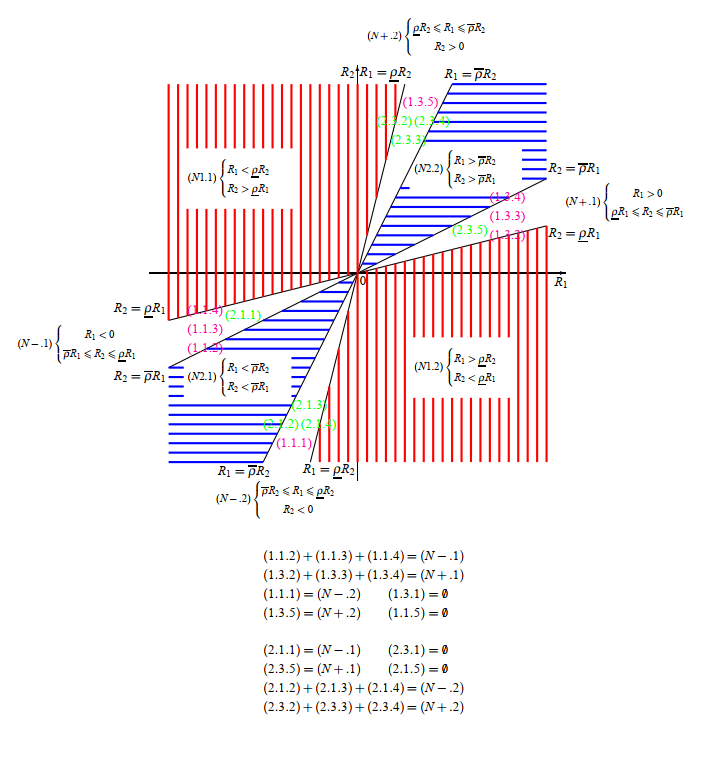
\includegraphics[width=1.1 \textwidth]{FigureA1.1.png}
\end{figure}

\vskip 64 pt



%\vskip 16 pt

\newpage




\begin{figure}
	\centerline{\bf Figure A1.2 \quad Solution zones for $ 0 = \underline{\rho} < \overline{\rho} $}
	\centering
	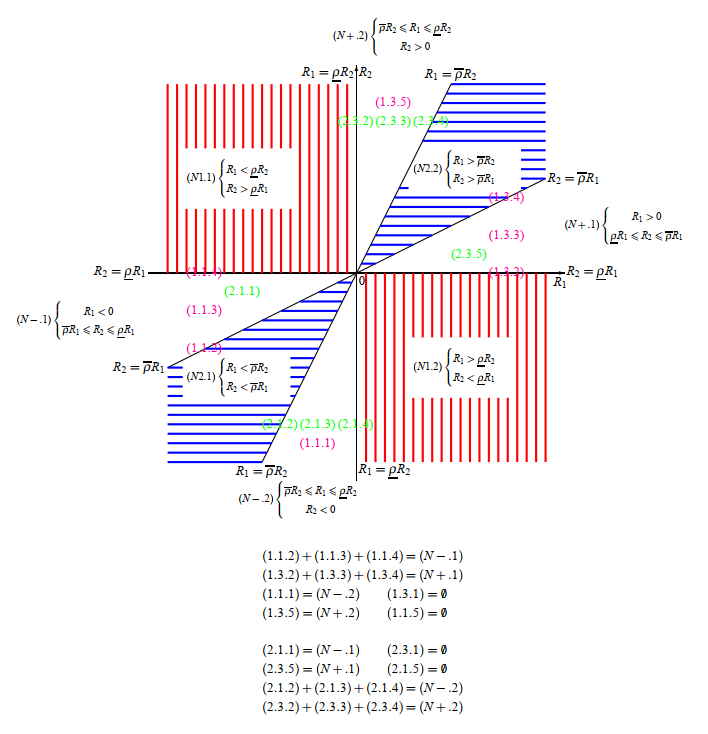
\includegraphics[width=1.1 \textwidth]{FigureA1.2.png}
\end{figure}

\vskip 64 pt



%\vskip 16 pt

\newpage


\begin{figure}
\centerline{\bf Figure A1.3 \quad Solution zones for $ \underline{\rho} < 0 < \overline{\rho} $}
	\centering
	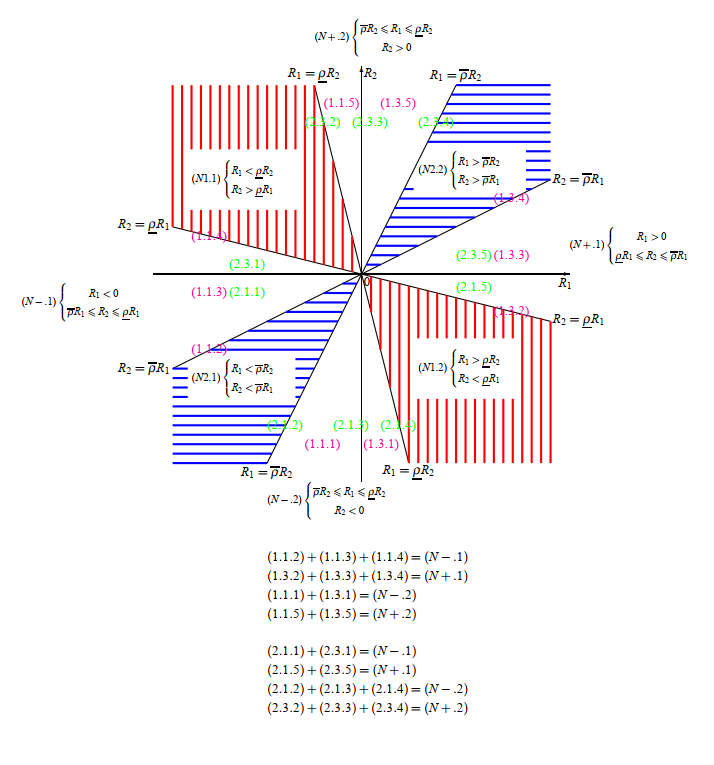
\includegraphics[width=1.1 \textwidth]{FigureA1.3.png}
\end{figure}
\vskip 64 pt


%\vskip 16 pt

\newpage


\begin{figure}
\centerline{\bf Figure A1.4 \quad Solution zones for $ \underline{\rho} < \overline{\rho} = 0 $}
	\centering
	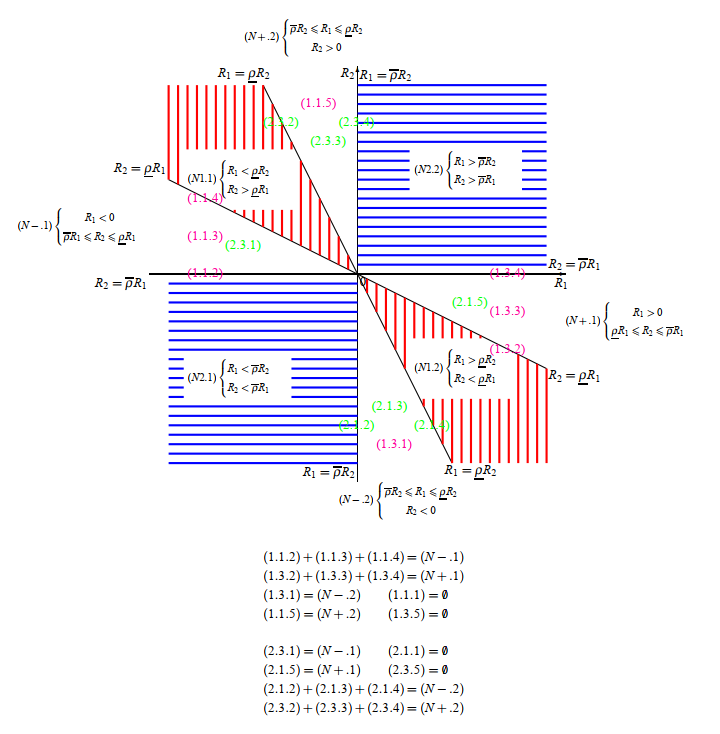
\includegraphics[width=1.1 \textwidth]{FigureA1.4.png}
\end{figure}
\vskip 64 pt


%\vskip 16 pt

\newpage


\begin{figure}
\centerline{\bf Figure A1.5 \quad Solution zones for $ \underline{\rho} < \overline{\rho} < 0 $}
	\centering
	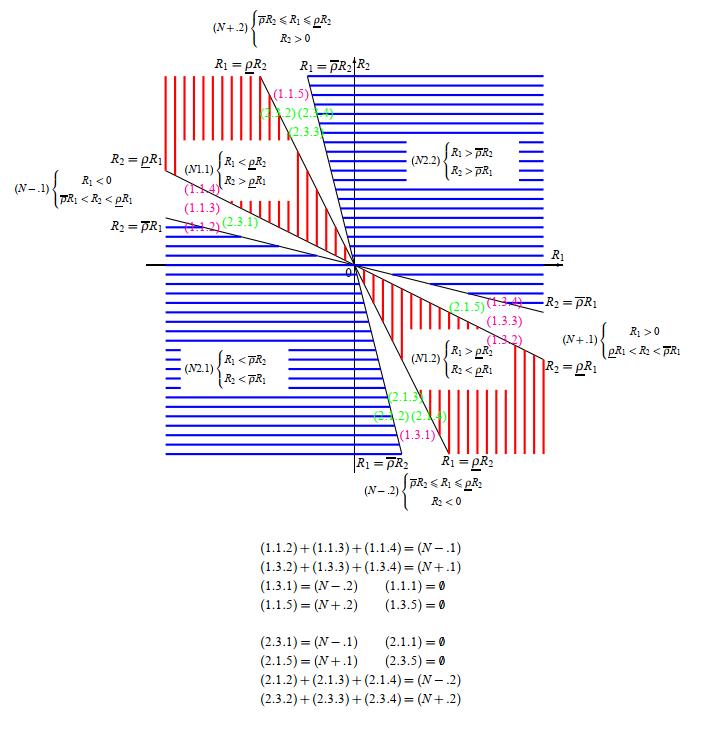
\includegraphics[width=1.1 \textwidth]{FigureA1.5.png}
\end{figure}
\vskip 64 pt

%\vskip 16 pt

\newpage

\subsection*{A.2 \quad 天真投资者的需求函数图}

\quad \


请注意,天真投资者对资产 $i$ 的需求取决于两种风险资产的价格,并且函数图的形状随 $R_i$ 的符号的变化而变化,因此很难描绘 $ Z (p_1, p_2) $ 在三维坐标空间中的图,所以我们采用比较静态分析的方法。由于两种资产的需求函数的形式是对称的,所以这里只给出资产 $1$ 的需求函数。 当研究资产 1 的需求 $ Z_1 (p_1) $如何随 $ p_1 $ 变化时,我们固定 $ p_2 $ 的值(并假设 $ R_2 $ 的符号)。

情况 1:资产 2 的价格高于平均收益,$ p_2 > \mu_2 $。 根据相关系数的不同边界,我们描绘了需求函数$Z_1(p_1)$。

对于 $ p_2 > \mu_2 $ 和 $ 0 < \underline{\rho} < \overline{\rho} $,
{\footnotesize \begin{eqnarray}
Z_{N 1}^* = \left\{ \begin{matrix}
\dfrac{\sigma_2^2 (\mu_1 - p_1) - \underline{\rho} \sigma_1 \sigma_2 (\mu_2 - p_2)}{\alpha \sigma_1^2 \sigma_2^2 (1 - \underline{\rho}^2)}, & \text{若} \qquad p_1 < \mu_1 - \underline{\rho} \dfrac{\sigma_1}{\sigma_2} (\mu_2 - p_2) \\
0, & \text{若} \qquad \mu_1 - \underline{\rho} \dfrac{\sigma_1}{\sigma_2} (\mu_2 - p_2) \leqslant p_1 \leqslant \mu_1 - \overline{\rho} \dfrac{\sigma_1}{\sigma_2} (\mu_2 - p_2) \\
\dfrac{\sigma_2^2 (\mu_1 - p_1) - \overline{\rho} \sigma_1 \sigma_2 (\mu_2 - p_2)}{\alpha \sigma_1^2 \sigma_2^2 (1 - \overline{\rho}^2)}, & \text{若} \qquad \mu_1 - \overline{\rho} \dfrac{\sigma_1}{\sigma_2} (\mu_2 - p_2) < p_1 < \mu_1 - \dfrac1{\overline{\rho}} \dfrac{\sigma_1}{\sigma_2} (\mu_2 - p_2) \\
\dfrac{\mu_1 - p_1}{\alpha \sigma_1^2}, & \text{若} \qquad \mu_1 - \dfrac1{\overline{\rho}} \dfrac{\sigma_1}{\sigma_2} (\mu_2 - p_2) \leqslant p_1 \leqslant \mu_1 - \dfrac1{\underline{\rho}} \dfrac{\sigma_1}{\sigma_2} (\mu_2 - p_2) \\
\dfrac{\sigma_2^2 (\mu_1 - p_1) - \underline{\rho} \sigma_1 \sigma_2 (\mu_2 - p_2)}{\alpha \sigma_1^2 \sigma_2^2 (1 - \underline{\rho}^2)}, & \text{若} \qquad \mu_1 - \dfrac1{\underline{\rho}} \dfrac{\sigma_1}{\sigma_2} (\mu_2 - p_2) < p_1.
\end{matrix} \right.
\end{eqnarray}}

对于 $ p_2 > \mu_2 $ 和 $ 0 = \underline{\rho} < \overline{\rho} $,
{\footnotesize \begin{eqnarray}
Z_{N 1}^* = \left\{ \begin{matrix}
\dfrac{\mu_1 - p_1}{\alpha \sigma_1^2}, & \text{若} \qquad p_1 < \mu_1 \\
0, & \text{若} \qquad \mu_1 \leqslant p_1 \leqslant \mu_1 - \overline{\rho} \dfrac{\sigma_1}{\sigma_2} (\mu_2 - p_2) \\
\dfrac{\sigma_2^2 (\mu_1 - p_1) - \overline{\rho} \sigma_1 \sigma_2 (\mu_2 - p_2)}{\alpha \sigma_1^2 \sigma_2^2 (1 - \overline{\rho}^2)}, & \text{若} \qquad \mu_1 - \overline{\rho} \dfrac{\sigma_1}{\sigma_2} (\mu_2 - p_2) < p_1 < \mu_1 - \dfrac1{\overline{\rho}} \dfrac{\sigma_1}{\sigma_2} (\mu_2 - p_2) \\
\dfrac{\mu_1 - p_1}{\alpha \sigma_1^2}, & \text{若} \qquad \mu_1 - \dfrac1{\overline{\rho}} \dfrac{\sigma_1}{\sigma_2} (\mu_2 - p_2) \leqslant p_1.
\end{matrix} \right.
\end{eqnarray}}

对于 $ p_2 > \mu_2 $ 和 $ \underline{\rho} < 0 < \overline{\rho} $,
{\footnotesize \begin{eqnarray}
Z_{N 1}^* = \left\{ \begin{matrix}
\dfrac{\mu_1 - p_1}{\alpha \sigma_1^2}, & \text{若} \qquad p_1 \leqslant \mu_1 - \dfrac1{\underline{\rho}} \dfrac{\sigma_1}{\sigma_2} (\mu_2 - p_2) \\
\dfrac{\sigma_2^2 (\mu_1 - p_1) - \underline{\rho} \sigma_1 \sigma_2 (\mu_2 - p_2)}{\alpha \sigma_1^2 \sigma_2^2 (1 - \underline{\rho}^2)}, & \text{若} \qquad \mu_1 - \dfrac1{\underline{\rho}} \dfrac{\sigma_1}{\sigma_2} (\mu_2 - p_2) < p_1 < \mu_1 - \underline{\rho} \dfrac{\sigma_1}{\sigma_2} (\mu_2 - p_2) \\
0, & \text{若} \qquad \mu_1 - \underline{\rho} \dfrac{\sigma_1}{\sigma_2} (\mu_2 - p_2) \leqslant p_1 \leqslant \mu_1 - \overline{\rho} \dfrac{\sigma_1}{\sigma_2} (\mu_2 - p_2) \\
\dfrac{\sigma_2^2 (\mu_1 - p_1) - \overline{\rho} \sigma_1 \sigma_2 (\mu_2 - p_2)}{\alpha \sigma_1^2 \sigma_2^2 (1 - \overline{\rho}^2)}, & \text{若} \qquad \mu_1 - \overline{\rho} \dfrac{\sigma_1}{\sigma_2} (\mu_2 - p_2) < p_1 < \mu_1 - \dfrac1{\overline{\rho}} \dfrac{\sigma_1}{\sigma_2} (\mu_2 - p_2) \\
\dfrac{\mu_1 - p_1}{\alpha \sigma_1^2}, & \text{若} \qquad \mu_1 - \dfrac1{\overline{\rho}} \dfrac{\sigma_1}{\sigma_2} (\mu_2 - p_2) \leqslant p_1.
\end{matrix} \right.
\end{eqnarray}}

对于 $ p_2 > \mu_2 $ 和 $ \underline{\rho} < \overline{\rho} = 0 $,
{\footnotesize \begin{eqnarray}
Z_{N 1}^* = \left\{ \begin{matrix}
\dfrac{\mu_1 - p_1}{\alpha \sigma_1^2}, & \text{若} \qquad p_1 \leqslant \mu_1 - \dfrac1{\underline{\rho}} \dfrac{\sigma_1}{\sigma_2} (\mu_2 - p_2) \\
\dfrac{\sigma_2^2 (\mu_1 - p_1) - \underline{\rho} \sigma_1 \sigma_2 (\mu_2 - p_2)}{\alpha \sigma_1^2 \sigma_2^2 (1 - \underline{\rho}^2)}, & \text{若} \qquad \mu_1 - \dfrac1{\underline{\rho}} \dfrac{\sigma_1}{\sigma_2} (\mu_2 - p_2) < p_1 < \mu_1 - \underline{\rho} \dfrac{\sigma_1}{\sigma_2} (\mu_2 - p_2) \\
0, & \text{若} \qquad \mu_1 - \underline{\rho} \dfrac{\sigma_1}{\sigma_2} (\mu_2 - p_2) \leqslant p_1 \leqslant \mu_1 \\
\dfrac{\mu_1 - p_1}{\alpha \sigma_1^2}, & \text{若} \qquad \qquad \mu_1 < p_1.
\end{matrix} \right.
\end{eqnarray}}

对于 $ p_2 > \mu_2 $ 和 $ \underline{\rho} < \overline{\rho} < 0 $,
{\footnotesize \begin{eqnarray}
Z_{N 1}^* = \left\{ \begin{matrix}
\dfrac{\sigma_2^2 (\mu_1 - p_1) - \overline{\rho} \sigma_1 \sigma_2 (\mu_2 - p_2)}{\alpha \sigma_1^2 \sigma_2^2 (1 - \overline{\rho}^2)}, & \text{若} \qquad p_1 < \mu_1 - \dfrac1{\overline{\rho}} \dfrac{\sigma_1}{\sigma_2} (\mu_2 - p_2) \\
\dfrac{\mu_1 - p_1}{\alpha \sigma_1^2}, & \text{若} \qquad \mu_1 - \dfrac1{\overline{\rho}} \dfrac{\sigma_1}{\sigma_2} (\mu_2 - p_2) \leqslant p_1 \leqslant \mu_1 - \dfrac1{\underline{\rho}} \dfrac{\sigma_1}{\sigma_2} (\mu_2 - p_2) \\
\dfrac{\sigma_2^2 (\mu_1 - p_1) - \underline{\rho} \sigma_1 \sigma_2 (\mu_2 - p_2)}{\alpha \sigma_1^2 \sigma_2^2 (1 - \underline{\rho}^2)}, & \text{若} \qquad \mu_1 - \dfrac1{\underline{\rho}} \dfrac{\sigma_1}{\sigma_2} (\mu_2 - p_2) < p_1 < \mu_1 - \underline{\rho} \dfrac{\sigma_1}{\sigma_2} (\mu_2 - p_2) \\
0, & \text{若} \qquad \mu_1 - \underline{\rho} \dfrac{\sigma_1}{\sigma_2} (\mu_2 - p_2) \leqslant p_1 \leqslant \mu_1 - \overline{\rho} \dfrac{\sigma_1}{\sigma_2} (\mu_2 - p_2) \\
\dfrac{\sigma_2^2 (\mu_1 - p_1) - \overline{\rho} \sigma_1 \sigma_2 (\mu_2 - p_2)}{\alpha \sigma_1^2 \sigma_2^2 (1 - \overline{\rho}^2)}, & \text{若} \qquad \qquad \mu_1 - \overline{\rho} \dfrac{\sigma_1}{\sigma_2} (\mu_2 - p_2) < p_1.
\end{matrix} \right.
\end{eqnarray}}



式 (A.9) 是式 (A.8) 和 (A.10) 在 $ \underline{\rho} = 0 $ 时的极限形式。
式 (A.11) 是式 (A.10) 和 (A.12) 在 $ \overline{\rho} = 0 $ 时的极限形式。
五种情况:$0 < \underline{\rho} < \overline{\rho} $, $ 0 = \underline{\rho} < \overline{\rho} $, $ \underline{\rho} < 0 < \overline{\rho} $, $ \underline{\rho} < \overline{\rho} = 0 $, $ \underline{\rho} < \overline{\rho} < 0 $如图A.2.1 - A.2.5所示。 有图可得需求函数 $ Z_1 (p_1) $ 是分段线性的并且关于 $ p_1 $ 单调递减。

情况 2:资产 2 的价格低于平均收益 $ p_2 < \mu_2 $。 根据相关系数的不同边界,我们描绘了需求函数$Z_1(p_1)$。

对于 $ p_2 < \mu_2 $ 和 $ 0 < \underline{\rho} < \overline{\rho} $,
{\footnotesize \begin{eqnarray}
Z_{N 1}^* = \left\{ \begin{matrix}
\dfrac{\sigma_2^2 (\mu_1 - p_1) - \underline{\rho} \sigma_1 \sigma_2 (\mu_2 - p_2)}{\alpha \sigma_1^2 \sigma_2^2 (1 - \underline{\rho}^2)}, & \text{若} \qquad p_1 < \mu_1 - \dfrac1{\underline{\rho}} \dfrac{\sigma_1}{\sigma_2} (\mu_2 - p_2) \\
\dfrac{\mu_1 - p_1}{\alpha \sigma_1^2}, & \text{若} \qquad \mu_1 - \dfrac1{\underline{\rho}} \dfrac{\sigma_1}{\sigma_2} (\mu_2 - p_2) \leqslant p_1 \leqslant \mu_1 - \dfrac1{\overline{\rho}} \dfrac{\sigma_1}{\sigma_2} (\mu_2 - p_2) \\
\dfrac{\sigma_2^2 (\mu_1 - p_1) - \overline{\rho} \sigma_1 \sigma_2 (\mu_2 - p_2)}{\alpha \sigma_1^2 \sigma_2^2 (1 - \overline{\rho}^2)}, & \text{若} \qquad \mu_1 - \dfrac1{\overline{\rho}} \dfrac{\sigma_1}{\sigma_2} (\mu_2 - p_2) < p_1 < \mu_1 - \overline{\rho} \dfrac{\sigma_1}{\sigma_2} (\mu_2 - p_2) \\
0, & \text{若} \qquad \mu_1 - \overline{\rho} \dfrac{\sigma_1}{\sigma_2} (\mu_2 - p_2) \leqslant p_1 \leqslant \mu_1 - \underline{\rho} \dfrac{\sigma_1}{\sigma_2} (\mu_2 - p_2) \\
\dfrac{\sigma_2^2 (\mu_1 - p_1) - \underline{\rho} \sigma_1 \sigma_2 (\mu_2 - p_2)}{\alpha \sigma_1^2 \sigma_2^2 (1 - \underline{\rho}^2)}, & \text{若} \qquad \mu_1 - \underline{\rho} \dfrac{\sigma_1}{\sigma_2} (\mu_2 - p_2) < p_1.
\end{matrix} \right.
\end{eqnarray}}

对于 $ p_2 < \mu_2 $ 和 $ 0 = \underline{\rho} < \overline{\rho} $,
{\footnotesize \begin{eqnarray}
Z_{N 1}^* = \left\{ \begin{matrix}
\dfrac{\mu_1 - p_1}{\alpha \sigma_1^2}, & \text{若} \qquad p_1 \leqslant \mu_1 - \dfrac1{\overline{\rho}} \dfrac{\sigma_1}{\sigma_2} (\mu_2 - p_2) \\
\dfrac{\sigma_2^2 (\mu_1 - p_1) - \overline{\rho} \sigma_1 \sigma_2 (\mu_2 - p_2)}{\alpha \sigma_1^2 \sigma_2^2 (1 - \overline{\rho}^2)}, & \text{若} \qquad \mu_1 - \dfrac1{\overline{\rho}} \dfrac{\sigma_1}{\sigma_2} (\mu_2 - p_2) < p_1 < \mu_1 - \overline{\rho} \dfrac{\sigma_1}{\sigma_2} (\mu_2 - p_2) \\
0, & \text{若} \qquad \mu_1 - \overline{\rho} \dfrac{\sigma_1}{\sigma_2} (\mu_2 - p_2) \leqslant p_1 \leqslant \mu_1 \\
\dfrac{\mu_1 - p_1}{\alpha \sigma_1^2}, & \text{若} \qquad \mu_1 < p_1.
\end{matrix} \right.
\end{eqnarray}}

对于 $ p_2 < \mu_2 $ 和 $ \underline{\rho} < 0 < \overline{\rho} $,
{\footnotesize \begin{eqnarray}
Z_{N 1}^* = \left\{ \begin{matrix}
\dfrac{\mu_1 - p_1}{\alpha \sigma_1^2}, & \text{若} \qquad p_1 \leqslant \mu_1 - \dfrac1{\overline{\rho}} \dfrac{\sigma_1}{\sigma_2} (\mu_2 - p_2) \\
\dfrac{\sigma_2^2 (\mu_1 - p_1) - \overline{\rho} \sigma_1 \sigma_2 (\mu_2 - p_2)}{\alpha \sigma_1^2 \sigma_2^2 (1 - \overline{\rho}^2)}, & \text{若} \qquad \mu_1 - \dfrac1{\overline{\rho}} \dfrac{\sigma_1}{\sigma_2} (\mu_2 - p_2) < p_1 < \mu_1 - \overline{\rho} \dfrac{\sigma_1}{\sigma_2} (\mu_2 - p_2) \\
0, & \text{若} \qquad \mu_1 - \overline{\rho} \dfrac{\sigma_1}{\sigma_2} (\mu_2 - p_2) \leqslant p_1 \leqslant \mu_1 - \underline{\rho} \dfrac{\sigma_1}{\sigma_2} (\mu_2 - p_2) \\
\dfrac{\sigma_2^2 (\mu_1 - p_1) - \underline{\rho} \sigma_1 \sigma_2 (\mu_2 - p_2)}{\alpha \sigma_1^2 \sigma_2^2 (1 - \underline{\rho}^2)}, & \text{若} \qquad \mu_1 - \underline{\rho} \dfrac{\sigma_1}{\sigma_2} (\mu_2 - p_2) < p_1 < \mu_1 - \dfrac1{\underline{\rho}} \dfrac{\sigma_1}{\sigma_2} (\mu_2 - p_2) \\
\dfrac{\mu_1 - p_1}{\alpha \sigma_1^2}, & \text{若} \qquad \mu_1 - \dfrac1{\underline{\rho}} \dfrac{\sigma_1}{\sigma_2} (\mu_2 - p_2) \leqslant p_1.
\end{matrix} \right.
\end{eqnarray}}

对于 $ p_2 < \mu_2 $ 和 $ \underline{\rho} < \overline{\rho} = 0 $,
{\footnotesize \begin{eqnarray}
Z_{N 1}^* = \left\{ \begin{matrix}
\dfrac{\mu_1 - p_1}{\alpha \sigma_1^2}, & \text{若} \qquad p_1 < \mu_1 \\
0, & \text{若} \qquad \mu_1 \leqslant p_1 \leqslant \mu_1 - \underline{\rho} \dfrac{\sigma_1}{\sigma_2} (\mu_2 - p_2) \\
\dfrac{\sigma_2^2 (\mu_1 - p_1) - \underline{\rho} \sigma_1 \sigma_2 (\mu_2 - p_2)}{\alpha \sigma_1^2 \sigma_2^2 (1 - \underline{\rho}^2)}, & \text{若} \qquad \mu_1 - \underline{\rho} \dfrac{\sigma_1}{\sigma_2} (\mu_2 - p_2) < p_1 < \mu_1 - \dfrac1{\underline{\rho}} \dfrac{\sigma_1}{\sigma_2} (\mu_2 - p_2) \\
\dfrac{\mu_1 - p_1}{\alpha \sigma_1^2}, & \text{若} \qquad \mu_1 - \dfrac1{\underline{\rho}} \dfrac{\sigma_1}{\sigma_2} (\mu_2 - p_2) \leqslant p_1.
\end{matrix} \right.
\end{eqnarray}}

对于 $ p_2 < \mu_2 $ 和 $ \underline{\rho} < \overline{\rho} < 0 $,
{\footnotesize \begin{eqnarray}
Z_{N 1}^* = \left\{ \begin{matrix}
\dfrac{\sigma_2^2 (\mu_1 - p_1) - \overline{\rho} \sigma_1 \sigma_2 (\mu_2 - p_2)}{\alpha \sigma_1^2 \sigma_2^2 (1 - \overline{\rho}^2)}, & \text{若} \qquad p_1 < \mu_1 - \overline{\rho} \dfrac{\sigma_1}{\sigma_2} (\mu_2 - p_2) \\
0, & \text{若} \qquad \mu_1 - \overline{\rho} \dfrac{\sigma_1}{\sigma_2} (\mu_2 - p_2) \leqslant p_1 \leqslant \mu_1 - \underline{\rho} \dfrac{\sigma_1}{\sigma_2} (\mu_2 - p_2) \\
\dfrac{\sigma_2^2 (\mu_1 - p_1) - \underline{\rho} \sigma_1 \sigma_2 (\mu_2 - p_2)}{\alpha \sigma_1^2 \sigma_2^2 (1 - \underline{\rho}^2)}, & \text{若} \qquad \mu_1 - \underline{\rho} \dfrac{\sigma_1}{\sigma_2} (\mu_2 - p_2) < p_1 < \mu_1 - \dfrac1{\underline{\rho}} \dfrac{\sigma_1}{\sigma_2} (\mu_2 - p_2) \\
\dfrac{\mu_1 - p_1}{\alpha \sigma_1^2}, & \text{若} \qquad \mu_1 - \dfrac1{\underline{\rho}} \dfrac{\sigma_1}{\sigma_2} (\mu_2 - p_2) \leqslant p_1 \leqslant \mu_1 - \dfrac1{\overline{\rho}} \dfrac{\sigma_1}{\sigma_2} (\mu_2 - p_2) \\
\dfrac{\sigma_2^2 (\mu_1 - p_1) - \overline{\rho} \sigma_1 \sigma_2 (\mu_2 - p_2)}{\alpha \sigma_1^2 \sigma_2^2 (1 - \overline{\rho}^2)}, & \text{若} \qquad \mu_1 - \dfrac1{\overline{\rho}} \dfrac{\sigma_1}{\sigma_2} (\mu_2 - p_2) < p_1.
\end{matrix} \right.
\end{eqnarray}}



式 (A.14) 是式 (A.13) 和 (A.15) 在 $ \underline{\rho} = 0 $ 时的极限形式。
式 (A.16) 是式 (A.15) 和 (A.17) 在 $ \overline{\rho} = 0 $ 时的极限形式。
五种情况:$0 < \underline{\rho} < \overline{\rho} $, $ 0 = \underline{\rho} < \overline{\rho} $, $ \underline{\rho} < 0 < \overline{\rho} $, $ \underline{\rho} < \overline{\rho} = 0 $, 和 $ \underline{\rho} < \overline{\rho} < 0 $ 如图 A.2.6 - A.2.10所示。 由图可得需求函数 $ Z_1 (p_1) $ 是分段线性的并且关于 $ p_1 $ 单调递减。

\vskip 8 pt


然后我们考虑资产 1 的需求$ Z_1 (p_2) $如何随 $ p_2 $ 变化,此时我们固定 $ p_1 $ 的值(并假设 $ R_1 $ 的符号)。

情形 1:资产 1 的价格高于平均收益,$ p_1 > \mu_1 $。 根据相关系数的不同界限,我们描绘了需求函数$Z_1 (p_2)$。


对于 $ p_1 > \mu_1 $ 和 $ 0 < \underline{\rho} < \overline{\rho} $,
{\footnotesize \begin{eqnarray}
Z_{N 1}^* = \left\{ \begin{matrix}
\dfrac{\sigma_2^2 (\mu_1 - p_1) - \underline{\rho} \sigma_1 \sigma_2 (\mu_2 - p_2)}{\alpha \sigma_1^2 \sigma_2^2 (1 - \underline{\rho}^2)}, & \text{若} \qquad p_2 < \mu_2 - \underline{\rho} \dfrac{\sigma_2}{\sigma_1} (\mu_1 - p_1) \\
\dfrac{\mu_1 - p_1}{\alpha \sigma_1^2}, & \text{若} \qquad \mu_2 - \underline{\rho} \dfrac{\sigma_2}{\sigma_1} (\mu_1 - p_1) \leqslant p_2 \leqslant \mu_2 - \overline{\rho} \dfrac{\sigma_2}{\sigma_1} (\mu_1 - p_1) \\
\dfrac{\sigma_2^2 (\mu_1 - p_1) - \overline{\rho} \sigma_1 \sigma_2 (\mu_2 - p_2)}{\alpha \sigma_1^2 \sigma_2^2 (1 - \overline{\rho}^2)}, & \text{若} \qquad \mu_2 - \overline{\rho} \dfrac{\sigma_2}{\sigma_1} (\mu_1 - p_1) < p_2 < \mu_2 - \dfrac1{\overline{\rho}} \dfrac{\sigma_2}{\sigma_1} (\mu_1 - p_1) \\
0, & \text{若} \qquad \mu_2 - \dfrac1{\overline{\rho}} \dfrac{\sigma_2}{\sigma_1} (\mu_1 - p_1) \leqslant p_2 \leqslant \mu_2 - \dfrac1{\underline{\rho}} \dfrac{\sigma_2}{\sigma_1} (\mu_1 - p_1) \\
\dfrac{\sigma_2^2 (\mu_1 - p_1) - \underline{\rho} \sigma_1 \sigma_2 (\mu_2 - p_2)}{\alpha \sigma_1^2 \sigma_2^2 (1 - \underline{\rho}^2)}, & \text{若} \qquad \mu_2 - \dfrac1{\underline{\rho}} \dfrac{\sigma_2}{\sigma_1} (\mu_1 - p_1) < p_2.
\end{matrix} \right.
\end{eqnarray}}

对于 $ p_1 > \mu_1 $ 和 $ 0 = \underline{\rho} < \overline{\rho} $,
{\footnotesize \begin{eqnarray}
Z_{N 1}^* = \left\{ \begin{matrix}
\dfrac{\mu_1 - p_1}{\alpha \sigma_1^2}, & \text{若} \qquad p_2 \leqslant \mu_2 - \overline{\rho} \dfrac{\sigma_2}{\sigma_1} (\mu_1 - p_1) \\
\dfrac{\sigma_2^2 (\mu_1 - p_1) - \overline{\rho} \sigma_1 \sigma_2 (\mu_2 - p_2)}{\alpha \sigma_1^2 \sigma_2^2 (1 - \overline{\rho}^2)}, & \text{若} \qquad \mu_2 - \overline{\rho} \dfrac{\sigma_2}{\sigma_1} (\mu_1 - p_1) < p_2 < \mu_2 - \dfrac1{\overline{\rho}} \dfrac{\sigma_2}{\sigma_1} (\mu_1 - p_1) \\
0, & \text{若} \qquad \mu_2 - \dfrac1{\overline{\rho}} \dfrac{\sigma_2}{\sigma_1} (\mu_1 - p_1) \leqslant p_2.
\end{matrix} \right.
\end{eqnarray}}

对于 $ p_1 > \mu_1 $ 和 $ \underline{\rho} < 0 < \overline{\rho} $,
{\footnotesize \begin{eqnarray}
Z_{N 1}^* = \left\{ \begin{matrix}
0, & \text{若} \qquad p_2 \leqslant \mu_2 - \dfrac1{\underline{\rho}} \dfrac{\sigma_2}{\sigma_1} (\mu_1 - p_1) \\
\dfrac{\sigma_2^2 (\mu_1 - p_1) - \underline{\rho} \sigma_1 \sigma_2 (\mu_2 - p_2)}{\alpha \sigma_1^2 \sigma_2^2 (1 - \underline{\rho}^2)}, & \text{若} \qquad \mu_2 - \dfrac1{\underline{\rho}} \dfrac{\sigma_2}{\sigma_1} (\mu_1 - p_1) < p_2 < \mu_2 - \underline{\rho} \dfrac{\sigma_2}{\sigma_1} (\mu_1 - p_1) \\
\dfrac{\mu_1 - p_1}{\alpha \sigma_1^2}, & \text{若} \qquad \mu_2 - \underline{\rho} \dfrac{\sigma_2}{\sigma_1} (\mu_1 - p_1) \leqslant p_2 \leqslant \mu_2 - \overline{\rho} \dfrac{\sigma_2}{\sigma_1} (\mu_1 - p_1) \\
\dfrac{\sigma_2^2 (\mu_1 - p_1) - \overline{\rho} \sigma_1 \sigma_2 (\mu_2 - p_2)}{\alpha \sigma_1^2 \sigma_2^2 (1 - \overline{\rho}^2)}, & \text{若} \qquad \mu_2 - \overline{\rho} \dfrac{\sigma_2}{\sigma_1} (\mu_1 - p_1) < p_2 < \mu_2 - \dfrac1{\overline{\rho}} \dfrac{\sigma_2}{\sigma_1} (\mu_1 - p_1) \\
0, & \text{若} \qquad \mu_2 - \dfrac1{\overline{\rho}} \dfrac{\sigma_2}{\sigma_1} (\mu_1 - p_1) \leqslant p_2.
\end{matrix} \right.
\end{eqnarray}}

对于 $ p_1 > \mu_1 $ 和 $ \underline{\rho} < \overline{\rho} = 0 $,
{\footnotesize \begin{eqnarray}
Z_{N 1}^* = \left\{ \begin{matrix}
0, & \text{若} \qquad p_2 \leqslant \mu_2 - \dfrac1{\underline{\rho}} \dfrac{\sigma_2}{\sigma_1} (\mu_1 - p_1) \\
\dfrac{\sigma_2^2 (\mu_1 - p_1) - \underline{\rho} \sigma_1 \sigma_2 (\mu_2 - p_2)}{\alpha \sigma_1^2 \sigma_2^2 (1 - \underline{\rho}^2)}, & \text{若} \qquad \mu_2 - \dfrac1{\underline{\rho}} \dfrac{\sigma_2}{\sigma_1} (\mu_1 - p_1) < p_2 < \mu_2 - \underline{\rho} \dfrac{\sigma_2}{\sigma_1} (\mu_1 - p_1) \\
\dfrac{\mu_1 - p_1}{\alpha \sigma_1^2}, & \text{若} \qquad \mu_2 - \underline{\rho} \dfrac{\sigma_2}{\sigma_1} (\mu_1 - p_1) \leqslant p_2.
\end{matrix} \right.
\end{eqnarray}}

对于 $ p_1 > \mu_1 $ 和 $ \underline{\rho} < \overline{\rho} < 0 $,
{\footnotesize \begin{eqnarray}
Z_{N 1}^* = \left\{ \begin{matrix}
\dfrac{\sigma_2^2 (\mu_1 - p_1) - \overline{\rho} \sigma_1 \sigma_2 (\mu_2 - p_2)}{\alpha \sigma_1^2 \sigma_2^2 (1 - \overline{\rho}^2)}, & \text{若} \qquad p_2 < \mu_2 - \dfrac1{\overline{\rho}} \dfrac{\sigma_2}{\sigma_1} (\mu_1 - p_1) \\
0, & \text{若} \qquad \mu_2 - \dfrac1{\overline{\rho}} \dfrac{\sigma_2}{\sigma_1} (\mu_1 - p_1) \leqslant p_2 \leqslant \mu_2 - \dfrac1{\underline{\rho}} \dfrac{\sigma_2}{\sigma_1} (\mu_1 - p_1) \\
\dfrac{\sigma_2^2 (\mu_1 - p_1) - \underline{\rho} \sigma_1 \sigma_2 (\mu_2 - p_2)}{\alpha \sigma_1^2 \sigma_2^2 (1 - \underline{\rho}^2)}, & \text{若} \qquad \mu_2 - \dfrac1{\underline{\rho}} \dfrac{\sigma_2}{\sigma_1} (\mu_1 - p_1) < p_2 < \mu_2 - \underline{\rho} \dfrac{\sigma_2}{\sigma_1} (\mu_1 - p_1) \\
\dfrac{\mu_1 - p_1}{\alpha \sigma_1^2}, & \text{若} \qquad \mu_2 - \underline{\rho} \dfrac{\sigma_2}{\sigma_1} (\mu_1 - p_1) \leqslant p_2 \leqslant \mu_2 - \overline{\rho} \dfrac{\sigma_2}{\sigma_1} (\mu_1 - p_1) \\
\dfrac{\sigma_2^2 (\mu_1 - p_1) - \overline{\rho} \sigma_1 \sigma_2 (\mu_2 - p_2)}{\alpha \sigma_1^2 \sigma_2^2 (1 - \overline{\rho}^2)}, & \text{若} \qquad \mu_2 - \overline{\rho} \dfrac{\sigma_2}{\sigma_1} (\mu_1 - p_1) < p_2.
\end{matrix} \right.
\end{eqnarray}}



式 (A.19) 是式 (A.18) 和 (A.20) 在 $ \underline{\rho} = 0 $ 时的极限形式。
式 (A.21) 是式 (A.20) 和 (A.22) 在 $ \overline{\rho} = 0 $ 时的极限形式。
图 A2.11 - A2.15 展示了五种情况:  $ 0 < \underline{\rho} < \overline{\rho} $, $ 0 = \underline{\rho} < \overline{\rho} $, $ \underline{\rho} < 0 < \overline{\rho} $, $ \underline{\rho} < \overline{\rho} = 0 $, 和 $ \underline{\rho} < \overline{\rho} < 0 $。由图可得需求函数 $ Z_1 (p_2) $ 是分段线性的,但其单调性取决于相关系数的端点值。天真投资者的需求函数 $ Z_1 (p_2) $ 在 $ 0 \leqslant \underline{\rho} < \overline{\rho} $ 上关于 $ p_2 $ 单调递增,在 $ \underline{\rho} < \overline{\rho} \leqslant 0 $ 上关于 $ p_2 $ 单调递减。

但是在$ \underline{\rho} < 0 < \overline{\rho} $上,它不是单调的。实际上它在$ \mu_2 - \dfrac1{\underline{\rho}} \dfrac{\sigma_2}{\sigma_1} (\mu_1 - p_1) $ 和 $ \mu_2 - \dfrac1{\overline{\rho}} \dfrac{\sigma_2}{\sigma_1} (\mu_1 - p_1) $ 之间是凸的,在此之外等于零(精明投资者的需求函数的斜率取决于 $ \hat{\rho} $ 的值。如果 $ \hat{\rho} > 0 $, $ \hat{\rho} = 0 $, $ \hat{\rho} < 0 $,则精明投资者的需求函数是一条递增、恒定、递减的直线,斜率分别为正$ \hat{ \rho} $、零、负 $ \hat{ \rho} $)。

情形 2:资产 1 的价格低于平均收益,$ p_1 < \mu_1 $。根据相关系数的不同的边界,我们描绘了需求函数$Z_1(p_2)$。


对于 $ p_1 < \mu_1 $ 和 $ 0 < \underline{\rho} < \overline{\rho} $,
{\footnotesize \begin{eqnarray}
Z_{N 1}^* = \left\{ \begin{matrix}
\dfrac{\sigma_2^2 (\mu_1 - p_1) - \underline{\rho} \sigma_1 \sigma_2 (\mu_2 - p_2)}{\alpha \sigma_1^2 \sigma_2^2 (1 - \underline{\rho}^2)}, & \text{若} \qquad p_2 < \mu_2 - \dfrac1{\underline{\rho}} \dfrac{\sigma_2}{\sigma_1} (\mu_1 - p_1) \\
0, & \text{若} \qquad \mu_2 - \dfrac1{\underline{\rho}} \dfrac{\sigma_2}{\sigma_1} (\mu_1 - p_1) \leqslant p_2 \leqslant \mu_2 - \dfrac1{\overline{\rho}} \dfrac{\sigma_2}{\sigma_1} (\mu_1 - p_1) \\
\dfrac{\sigma_2^2 (\mu_1 - p_1) - \overline{\rho} \sigma_1 \sigma_2 (\mu_2 - p_2)}{\alpha \sigma_1^2 \sigma_2^2 (1 - \overline{\rho}^2)}, & \text{若} \qquad \mu_2 - \dfrac1{\overline{\rho}} \dfrac{\sigma_2}{\sigma_1} (\mu_1 - p_1) < p_2 < \mu_2 - \overline{\rho} \dfrac{\sigma_2}{\sigma_1} (\mu_1 - p_1) \\
\dfrac{\mu_1 - p_1}{\alpha \sigma_1^2}, & \text{若} \qquad \mu_2 - \overline{\rho} \dfrac{\sigma_2}{\sigma_1} (\mu_1 - p_1) \leqslant p_2 \leqslant \mu_2 - \underline{\rho} \dfrac{\sigma_2}{\sigma_1} (\mu_1 - p_1) \\
\dfrac{\sigma_2^2 (\mu_1 - p_1) - \underline{\rho} \sigma_1 \sigma_2 (\mu_2 - p_2)}{\alpha \sigma_1^2 \sigma_2^2 (1 - \underline{\rho}^2)}, & \text{若} \qquad \mu_2 - \underline{\rho} \dfrac{\sigma_2}{\sigma_1} (\mu_1 - p_1) < p_2.
\end{matrix} \right.
\end{eqnarray}}

对于 $ p_1 < \mu_1 $ 和 $ 0 = \underline{\rho} < \overline{\rho} $,
{\footnotesize \begin{eqnarray}
Z_{N 1}^* = \left\{ \begin{matrix}
0, & \text{若} \qquad p_2 \leqslant \mu_2 - \dfrac1{\overline{\rho}} \dfrac{\sigma_2}{\sigma_1} (\mu_1 - p_1) \\
\dfrac{\sigma_2^2 (\mu_1 - p_1) - \overline{\rho} \sigma_1 \sigma_2 (\mu_2 - p_2)}{\alpha \sigma_1^2 \sigma_2^2 (1 - \overline{\rho}^2)}, & \text{若} \qquad \mu_2 - \dfrac1{\overline{\rho}} \dfrac{\sigma_2}{\sigma_1} (\mu_1 - p_1) < p_2 < \mu_2 - \overline{\rho} \dfrac{\sigma_2}{\sigma_1} (\mu_1 - p_1) \\
\dfrac{\mu_1 - p_1}{\alpha \sigma_1^2}, & \text{若} \qquad \mu_2 - \overline{\rho} \dfrac{\sigma_2}{\sigma_1} (\mu_1 - p_1) \leqslant p_2.
\end{matrix} \right.
\end{eqnarray}}

对于 $ p_1 < \mu_1 $ 和 $ \underline{\rho} < 0 < \overline{\rho} $,
{\footnotesize \begin{eqnarray}
Z_{N 1}^* = \left\{ \begin{matrix}
0, & \text{若} \qquad p_2 \leqslant \mu_2 - \dfrac1{\overline{\rho}} \dfrac{\sigma_2}{\sigma_1} (\mu_1 - p_1) \\
\dfrac{\sigma_2^2 (\mu_1 - p_1) - \overline{\rho} \sigma_1 \sigma_2 (\mu_2 - p_2)}{\alpha \sigma_1^2 \sigma_2^2 (1 - \overline{\rho}^2)}, & \text{若} \qquad \mu_2 - \dfrac1{\overline{\rho}} \dfrac{\sigma_2}{\sigma_1} (\mu_1 - p_1) < p_2 < \mu_2 - \overline{\rho} \dfrac{\sigma_2}{\sigma_1} (\mu_1 - p_1) \\
\dfrac{\mu_1 - p_1}{\alpha \sigma_1^2}, & \text{若} \qquad \mu_2 - \overline{\rho} \dfrac{\sigma_2}{\sigma_1} (\mu_1 - p_1) \leqslant p_2 \leqslant \mu_2 - \underline{\rho} \dfrac{\sigma_2}{\sigma_1} (\mu_1 - p_1) \\
\dfrac{\sigma_2^2 (\mu_1 - p_1) - \underline{\rho} \sigma_1 \sigma_2 (\mu_2 - p_2)}{\alpha \sigma_1^2 \sigma_2^2 (1 - \underline{\rho}^2)}, & \text{若} \qquad \mu_2 - \underline{\rho} \dfrac{\sigma_2}{\sigma_1} (\mu_1 - p_1) < p_2 < \mu_2 - \dfrac1{\underline{\rho}} \dfrac{\sigma_2}{\sigma_1} (\mu_1 - p_1) \\
0, & \text{若} \qquad \mu_2 - \dfrac1{\underline{\rho}} \dfrac{\sigma_2}{\sigma_1} (\mu_1 - p_1) \leqslant p_2.
\end{matrix} \right.
\end{eqnarray}}

对于 $ p_1 < \mu_1 $ 和 $ \underline{\rho} < \overline{\rho} = 0 $,
{\footnotesize \begin{eqnarray}
Z_{N 1}^* = \left\{ \begin{matrix}
\dfrac{\mu_1 - p_1}{\alpha \sigma_1^2}, & \text{若} \qquad p_2 \leqslant \mu_2 - \underline{\rho} \dfrac{\sigma_2}{\sigma_1} (\mu_1 - p_1) \\
\dfrac{\sigma_2^2 (\mu_1 - p_1) - \underline{\rho} \sigma_1 \sigma_2 (\mu_2 - p_2)}{\alpha \sigma_1^2 \sigma_2^2 (1 - \underline{\rho}^2)}, & \text{若} \qquad \mu_2 - \underline{\rho} \dfrac{\sigma_2}{\sigma_1} (\mu_1 - p_1) < p_2 < \mu_2 - \dfrac1{\underline{\rho}} \dfrac{\sigma_2}{\sigma_1} (\mu_1 - p_1) \\
0, & \text{若} \qquad \mu_2 - \dfrac1{\underline{\rho}} \dfrac{\sigma_2}{\sigma_1} (\mu_1 - p_1) \leqslant p_2.
\end{matrix} \right.
\end{eqnarray}}

对于 $ p_1 < \mu_1 $ 和 $ \underline{\rho} < \overline{\rho} < 0 $,
{\footnotesize \begin{eqnarray}
Z_{N 1}^* = \left\{ \begin{matrix}
\dfrac{\sigma_2^2 (\mu_1 - p_1) - \overline{\rho} \sigma_1 \sigma_2 (\mu_2 - p_2)}{\alpha \sigma_1^2 \sigma_2^2 (1 - \overline{\rho}^2)}, & \text{若} \qquad p_2 < \mu_2 - \overline{\rho} \dfrac{\sigma_2}{\sigma_1} (\mu_1 - p_1) \\
\dfrac{\mu_1 - p_1}{\alpha \sigma_1^2}, & \text{若} \qquad \mu_2 - \overline{\rho} \dfrac{\sigma_2}{\sigma_1} (\mu_1 - p_1) \leqslant p_2 \leqslant \mu_2 - \underline{\rho} \dfrac{\sigma_2}{\sigma_1} (\mu_1 - p_1) \\
\dfrac{\sigma_2^2 (\mu_1 - p_1) - \underline{\rho} \sigma_1 \sigma_2 (\mu_2 - p_2)}{\alpha \sigma_1^2 \sigma_2^2 (1 - \underline{\rho}^2)}, & \text{若} \qquad \mu_2 - \underline{\rho} \dfrac{\sigma_2}{\sigma_1} (\mu_1 - p_1) < p_2 < \mu_2 - \dfrac1{\underline{\rho}} \dfrac{\sigma_2}{\sigma_1} (\mu_1 - p_1) \\
0, & \text{若} \qquad \mu_2 - \dfrac1{\underline{\rho}} \dfrac{\sigma_2}{\sigma_1} (\mu_1 - p_1) \leqslant p_2 \leqslant \mu_2 - \dfrac1{\overline{\rho}} \dfrac{\sigma_2}{\sigma_1} (\mu_1 - p_1) \\
\dfrac{\sigma_2^2 (\mu_1 - p_1) - \overline{\rho} \sigma_1 \sigma_2 (\mu_2 - p_2)}{\alpha \sigma_1^2 \sigma_2^2 (1 - \overline{\rho}^2)}, & \text{若} \qquad \mu_2 - \dfrac1{\overline{\rho}} \dfrac{\sigma_2}{\sigma_1} (\mu_1 - p_1) < p_2.
\end{matrix} \right.
\end{eqnarray}}


式 (A.24) 是式 (A.23) 和 (A.25) 在 $ \underline{\rho} = 0 $ 时的极限形式。
式 (A.26) 是式 (A.25) 和 (A.27) 在 $ \overline{\rho} = 0 $ 时的极限形式。
图 A2.16 - A2.20 展示了五种情况:  $ 0 < \underline{\rho} < \overline{\rho} $, $ 0 = \underline{\rho} < \overline{\rho} $, $ \underline{\rho} < 0 < \overline{\rho} $, $ \underline{\rho} < \overline{\rho} = 0 $, $ \underline{\rho} < \overline{\rho} < 0 $。由图可得需求函数 $ Z_1 (p_2) $ 是分段线性的,但其单调性取决于相关系数的端点值。天真投资者的需求函数 $ Z_1 (p_2) $ 在 $ 0 \leqslant \underline{\rho} < \overline{\rho} $ 上关于 $ p_2 $ 单调递增,在  $ \underline{\rho} < \overline{\rho} \leqslant 0 $ 上关于 $ p_2 $ 单调递减。但是在$ \underline{\rho} < 0 < \overline{\rho} $上,它不是单调的。实际上在$ \mu_2 - \dfrac1{\overline{\rho}} \dfrac{\sigma_2}{\sigma_1} (\mu_1 - p_1) $ 和 $ \mu_2 - \dfrac1{\underline{\rho}} \dfrac{\sigma_2}{\sigma_1} (\mu_1 - p_1) $  之间是凹的,并且在此之外是零(精明投资者的需求函数的斜率取决于 $ \hat{\rho} $ 的值。如果 $ \hat{\rho} > 0 $, $ \hat{\rho} = 0 $, $ \hat{\rho} < 0 $,则精明投资者的需求函数是一条递增、恒定、递减的直线,斜率分别为正$ \hat{\rho} $、零、负 $ \hat{\rho} $)。





\newpage 
\begin{figure}
\centerline{\bf Figure A2.1 \quad Na\"ive tnvestor's demand function for given $ p_2 > \mu_2 $ and $ 0 < \underline{\rho} < \overline{\rho} $}
	\centering
	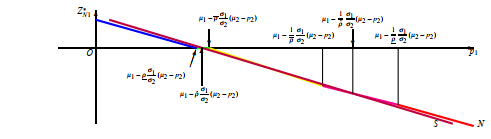
\includegraphics[width=1.0 \textwidth]{FigureA2.1.png}
\end{figure}

\vskip 16 pt


\begin{figure}
\centerline{\bf Figure A2.2 \quad Na\"ive tnvestor's demand function for given $ p_2 > \mu_2 $ and $ 0 = \underline{\rho} < \overline{\rho} $}
	\centering
	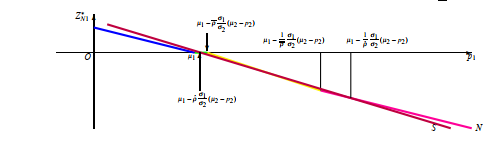
\includegraphics[width=1.0 \textwidth]{FigureA2.2.png}
\end{figure}

\vskip 16 pt



\begin{figure}
\centerline{\bf Figure A2.3 \quad Na\"ive tnvestor's demand function for given $ p_2 > \mu_2 $ and $ \underline{\rho} < 0 < \overline{\rho} $}
	\centering
	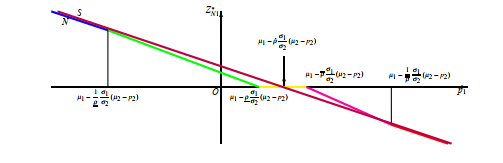
\includegraphics[width=1.0 \textwidth]{FigureA2.3.png}
\end{figure}


%\vskip 16 pt



\begin{figure}
\centerline{\bf Figure A2.4 \quad Na\"ive tnvestor's demand function for given $ p_2 > \mu_2 $ and $ \underline{\rho} < \overline{\rho} = 0 $}
	\centering
	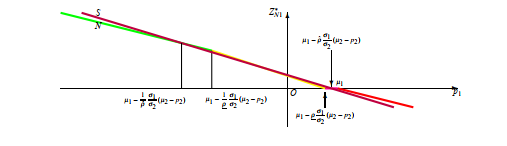
\includegraphics[width=1.0 \textwidth]{FigureA2.4.png}
\end{figure}




\vskip 16 pt


\begin{figure}
\centerline{\bf Figure A2.5 \quad Na\"ive tnvestor's demand function for given $ p_2 > \mu_2 $ and $ \underline{\rho} < \overline{\rho} < 0 $}
	\centering
	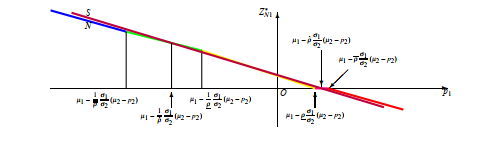
\includegraphics[width=1.0 \textwidth]{FigureA2.5.png}
\end{figure}

\newpage



\begin{figure}
\centerline{\bf Figure A2.6 \quad Na\"ive tnvestor's demand function for given $ p_2 < \mu_2 $ and $ 0 < \underline{\rho} < \overline{\rho} $}
	\centering
	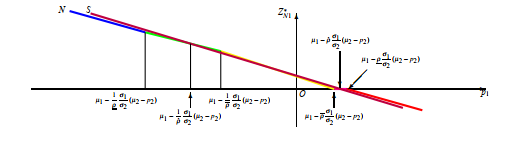
\includegraphics[width=1.0 \textwidth]{FigureA2.6.png}
\end{figure}


\vskip 8 pt


\begin{figure}
\centerline{\bf Figure A2.7 \quad Na\"ive tnvestor's demand function for given $ p_2 < \mu_2 $ and $ 0 = \underline{\rho} < \overline{\rho} $}
	\centering
	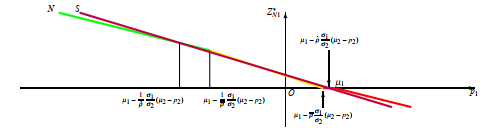
\includegraphics[width=1.0 \textwidth]{FigureA2.7.png}
\end{figure}


\vskip 8 pt


\begin{figure}
\centerline{\bf Figure A2.8 \quad Na\"ive tnvestor's demand function for given $ p_2 < \mu_2 $ and $ \underline{\rho} < 0 < \overline{\rho} $}
	\centering
	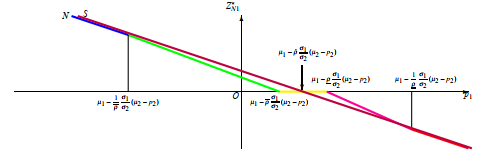
\includegraphics[width=1.0 \textwidth]{FigureA2.8.png}
\end{figure}



%\vskip 16 pt


\begin{figure}
\centerline{\bf Figure A2.9 \quad Na\"ive tnvestor's demand function for given $ p_2 < \mu_2 $ and $ \underline{\rho} < \overline{\rho} = 0 $}
	\centering
	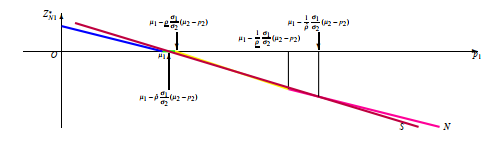
\includegraphics[width=1.0 \textwidth]{FigureA2.9.png}
\end{figure}



\vskip 8 pt



\begin{figure}
\centerline{\bf Figure A2.10 \quad Na\"ive tnvestor's demand function for given $ p_2 < \mu_2 $ and $ \underline{\rho} < \overline{\rho} < 0 $}
	\centering
	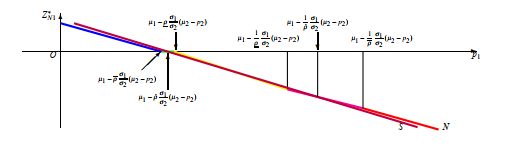
\includegraphics[width=1.0 \textwidth]{FigureA2.10.png}
\end{figure}



\newpage


\begin{figure}
\centerline{\bf Figure A2.11 \quad Na\"ive tnvestor's demand function for given $ p_1 > \mu_1 $ and $ 0 < \underline{\rho} < \overline{\rho} $}
	\centering
	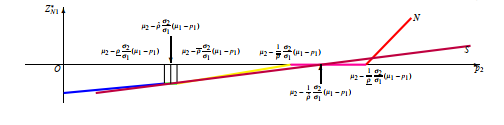
\includegraphics[width=1.0 \textwidth]{FigureA2.11.png}
\end{figure}




\begin{figure}
\centerline{\bf Figure A2.12 \quad Na\"ive tnvestor's demand function for given $ p_1 > \mu_1 $ and $ 0 = \underline{\rho} < \overline{\rho} $}
	\centering
	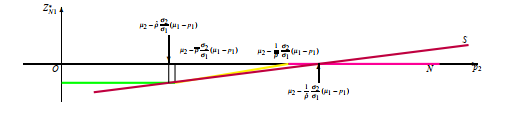
\includegraphics[width=1.0 \textwidth]{FigureA2.12.png}
\end{figure}



\begin{figure}
\centerline{\bf Figure A2.13 \quad Na\"ive tnvestor's demand function for given $ p_1 > \mu_1 $ and $ \underline{\rho} < 0 < \overline{\rho} $}
	\centering
	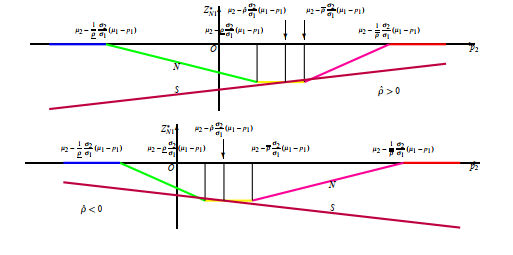
\includegraphics[width=1.0 \textwidth]{FigureA2.13.png}
\end{figure}



\begin{figure}
\centerline{\bf Figure A2.14 \quad Na\"ive tnvestor's demand function for given $ p_1 > \mu_1 $ and $ \underline{\rho} < \overline{\rho} = 0 $}
	\centering
	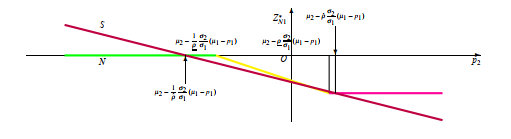
\includegraphics[width=1.0 \textwidth]{FigureA2.14.png}
\end{figure}



\begin{figure}
\centerline{\bf Figure A2.15 \quad Na\"ive tnvestor's demand function for given $ p_1 > \mu_1 $ and $ \underline{\rho} < \overline{\rho} < 0 $}
	\centering
	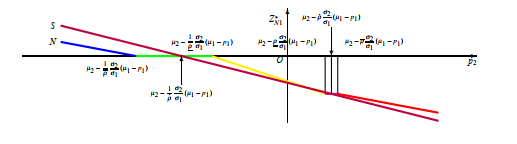
\includegraphics[width=1.0 \textwidth]{FigureA2.15.png}
\end{figure}

\newpage


\begin{figure}
\centerline{\bf Figure A2.16 \quad Na\"ive tnvestor's demand function for given $ p_1 < \mu_1 $ and $ 0 < \underline{\rho} < \overline{\rho} $}
	\centering
	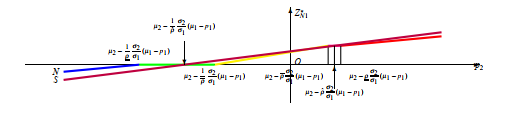
\includegraphics[width=1.0 \textwidth]{FigureA2.16.png}
\end{figure}



\begin{figure}
\centerline{\bf Figure A2.17 \quad Na\"ive tnvestor's demand function for given $ p_1 < \mu_1 $ and $ 0 = \underline{\rho} < \overline{\rho} $}
	\centering
	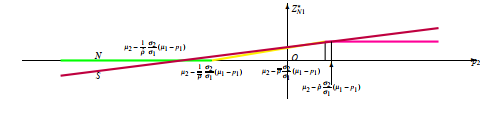
\includegraphics[width=1.0 \textwidth]{FigureA2.17.png}
\end{figure}



\begin{figure}
\centerline{\bf Figure A2.18 \quad Na\"ive tnvestor's demand function for given $ p_1 < \mu_1 $ and $ \underline{\rho} < 0 < \overline{\rho} $}
	\centering
	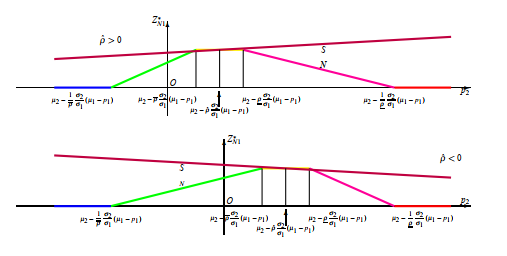
\includegraphics[width=1.0 \textwidth]{FigureA2.18.png}
\end{figure}



%\vskip 16 pt


\begin{figure}
\centerline{\bf Figure A2.19 \quad Na\"ive tnvestor's demand function for given $ p_1 < \mu_1 $ and $ \underline{\rho} < \overline{\rho} = 0 $}
	\centering
	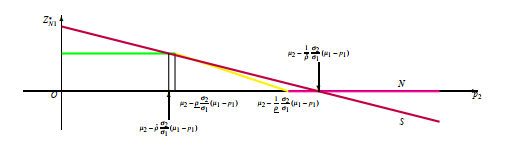
\includegraphics[width=1.0 \textwidth]{FigureA2.19.png}
\end{figure}



\begin{figure}
\centerline{\bf Figure A2.20 \quad Na\"ive tnvestor's demand function for given $ p_1 < \mu_1 $ and $ \underline{\rho} < \overline{\rho} < 0 $}
	\centering
	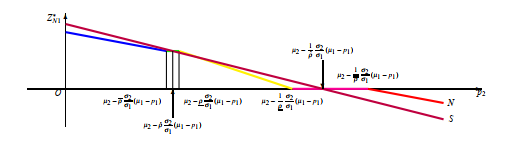
\includegraphics[width=1.0 \textwidth]{FigureA2.20.png}
\end{figure}





Easley 和 O'Hara (2009) 声称,精明投资者总是比天真投资者持有更多的风险资产(绝对值),因为对于任何给定的参数,这些投资者都会在均值和方差之间进行权衡。\footnote{\baselineskip1.3em 精明投资者和天真投资者都在规避风险,并在预期收益中为承担风险而要求补偿。然而,天真投资者也避免了收益分布的暧昧性,因此只要可能的均值和方差的集合是非退化的,他就会进一步减少风险资产的头寸。}但这在我们的式 (10) 以及图 A2.1 - A2.10 和 A2.11 - A2.20 中不成立。\footnote{\baselineskip1.3em 当我们观察两类投资者的需求曲线时,这是一个有趣且反直觉的特征。} 图 A2.1 - A2.20 表明,精明投资者的需求函数与天真投资者的需求函数在一定的价格区间上相交。具体而言,图 A2.1 - A2.10 报告了精明投资者的需求函数与天真投资者的需求函数在某一区间上相交:

对于 $ p_2 < \mu_2 $ ,交于区间
$$ \left[ \mu_1 - \overline{\rho} \dfrac{\sigma_1}{\sigma_2} (\mu_2 - p_2), \mu_1 - \underline{\rho} \dfrac{\sigma_1}{\sigma_2} (\mu_2 - p_2) \right] \ \text{和} \ \left[ \mu_1 - \dfrac1{\underline{\rho}} \dfrac{\sigma_1}{\sigma_2} (\mu_2 - p_2), \mu_1 - \dfrac1{\overline{\rho}} \dfrac{\sigma_1}{\sigma_2} (\mu_2 - p_2) \right] $$


对于 $ p_2 > \mu_2 $ ,交于区间
$$ \left[ \mu_1 - \underline{\rho} \dfrac{\sigma_1}{\sigma_2} (\mu_2 - p_2), \mu_1 - \overline{\rho} \dfrac{\sigma_1}{\sigma_2} (\mu_2 - p_2) \right] \ \text{和} \ \left[ \mu_1 - \dfrac1{\overline{\rho}} \dfrac{\sigma_1}{\sigma_2} (\mu_2 - p_2), \mu_1 - \dfrac1{\underline{\rho}} \dfrac{\sigma_1}{\sigma_2} (\mu_2 - p_2) \right] $$

图 A2.11 - A2.20 说明了精明投资者的需求函数与天真投资者的需求函数在某一区间上相交:
对于 $ p_1 < \mu_1 $ ,交于区间
$$ \left[ \mu_2 - \overline{\rho} \dfrac{\sigma_2}{\sigma_1} (\mu_1 - p_1), \mu_2 - \underline{\rho} \dfrac{\sigma_2}{\sigma_1} (\mu_1 - p_1) \right] \ \text{和} \ \left[ \mu_2 - \dfrac1{\underline{\rho}} \dfrac{\sigma_2}{\sigma_1} (\mu_1 - p_1), \mu_2 - \dfrac1{\overline{\rho}} \dfrac{\sigma_2}{\sigma_1} (\mu_1 - p_1) \right] $$
对于 $ p_1 > \mu_1 $ ,交于区间
$$ \left[ \mu_2 - \underline{\rho} \dfrac{\sigma_2}{\sigma_1} (\mu_1 - p_1), \mu_2 - \overline{\rho} \dfrac{\sigma_2}{\sigma_1} (\mu_1 - p_1) \right] \ \text{和} \ \left[ \mu_2 - \dfrac1{\overline{\rho}} \dfrac{\sigma_2}{\sigma_1} (\mu_1 - p_1), \mu_2 - \dfrac1{\underline{\rho}} \dfrac{\sigma_2}{\sigma_1} (\mu_1 - p_1) \right] $$


因此,在上述区间内,精明投资者可能并不总是比天真投资者持有更多的风险资产(绝对值)。这表明,厌恶暧昧性的投资者可能不像有的文献描述的那样,有时相关系数暧昧性的端点值有助于天真投资者选择正确的投资策略。

%\newpage

\subsection*{A.3 \quad 命题1的证明}

\quad \


精明投资者对风险资产的需求函数可以改写为:
{\small \begin{eqnarray}
Z_S^* = \left( \begin{matrix} Z_{S 1}^* \\ Z_{S 2}^* \end{matrix} \right) = \left\{ \begin{matrix}
\dfrac1{\alpha (1 - {\hat \rho}^2)} \left( \begin{matrix} \dfrac{R_1 - {\hat \rho} R_2}{\sigma_1} \\ \dfrac{R_2 - {\hat \rho} R_1}{\sigma_2} \end{matrix} \right), & \text{若} \quad (S1.1) \left\{ \begin{matrix} R_1 < {\hat \rho} R_2 \\ R_2 > {\hat \rho} R_1 \end{matrix} \right. \quad \text{或} \quad (S1.2) \left\{ \begin{matrix} R_1 > {\hat \rho} R_2 \\ R_2 < {\hat \rho} R_1 \end{matrix} \right. \\
\dfrac1{\alpha} \left( \begin{matrix} 0 \\ \dfrac{R_2}{\sigma_2} \end{matrix} \right), & \text{若} \quad (S-.2) \left\{ \begin{matrix} R_1 = {\hat \rho} R_2 \\ R_2 < 0 \end{matrix} \right. \quad \text{或} \quad (S+.2) \left\{ \begin{matrix} R_1 = {\hat \rho} R_2 \\ R_2 > 0 \end{matrix} \right. \\
\dfrac1{\alpha} \left( \begin{matrix} \dfrac{R_1}{\sigma_1} \\ 0 \end{matrix} \right), & \text{若} \quad (S-.1) \left\{ \begin{matrix} R_1 < 0 \\ R_2 = {\hat \rho} R_1 \end{matrix} \right. \quad \text{或} \quad (S+.1) \left\{ \begin{matrix} R_1 > 0 \\ R_2 = {\hat \rho} R_1 \end{matrix} \right. \\
\dfrac1{\alpha (1 - {\hat \rho}^2)} \left( \begin{matrix} \dfrac{R_1 - {\hat \rho} R_2}{\sigma_1} \\ \dfrac{R_2 - {\hat \rho} R_1}{\sigma_2} \end{matrix} \right), & \text{若} \quad (S2.1) \left\{ \begin{matrix} R_1 < {\hat \rho} R_2 \\ R_2 < {\hat \rho} R_1 \end{matrix} \right. \quad \text{或} \quad (S2.2) \left\{ \begin{matrix} R_1 > {\hat \rho} R_2 \\ R_2 > {\hat \rho} R_1. \end{matrix} \right.
\end{matrix} \right.
\end{eqnarray}}

\noindent 从式(6),平面 $ R_1 - O - R_2 $ 被(A.28)分为八个区域。 此外,
\begin{eqnarray*}
& Z_{S1}^* < 0 \quad \text{和} \quad Z_{S2}^* > 0 \quad \text{in} \quad (S1.1) & \\
& Z_{S1}^* > 0 \quad \text{和} \quad Z_{S2}^* < 0 \quad \text{in} \quad (S1.2) & \\
& Z_{S1}^* < 0 \quad \text{和} \quad Z_{S2}^* < 0 \quad \text{in} \quad (S2.1) & \\
& Z_{S1}^* > 0 \quad \text{和} \quad Z_{S2}^* > 0 \quad \text{in} \quad (S2.2) & 
\end{eqnarray*}
和
\begin{eqnarray*}
& Z_{S1}^* < 0 \quad \text{和} \quad Z_{S2}^* = 0 \quad \text{in} \quad (S-.1) & \\
& Z_{S1}^* > 0 \quad \text{和} \quad Z_{S2}^* = 0 \quad \text{in} \quad (S+.1) & \\
& Z_{S1}^* = 0 \quad \text{和} \quad Z_{S2}^* < 0 \quad \text{in} \quad (S-.2) & \\
& Z_{S1}^* = 0 \quad \text{和} \quad Z_{S2}^* > 0 \quad \text{in} \quad (S+.2). &
\end{eqnarray*}

因此
\begin{eqnarray*}
(N1.1) \subseteq (S1.1) & \qquad & (S-.1) \subseteq (N-.1) \\
(N1.2) \subseteq (S1.2) & \qquad & (S+.1) \subseteq (N+.1) \\
(N2.1) \subseteq (S2.1) & \qquad & (S-.2) \subseteq (N-.2) \\
(N2.2) \subseteq (S2.2) & \qquad & (S+.2) \subseteq (N+.2), 
\end{eqnarray*}
然后
\begin{eqnarray*}
Z_{N1}^* < 0 \quad \text{和} \quad Z_{N2}^* > 0 \quad & & \quad Z_{S1}^* < 0 \quad \text{和} \quad Z_{S2}^* > 0 \quad \text{in} \quad (N1.1) \\
Z_{N1}^* > 0 \quad \text{和} \quad Z_{N2}^* < 0 \quad & & \quad Z_{S1}^* > 0 \quad \text{和} \quad Z_{S2}^* < 0 \quad \text{in} \quad (N1.2) \\
Z_{N1}^* < 0 \quad \text{和} \quad Z_{N2}^* < 0 \quad & & \quad Z_{S1}^* < 0 \quad \text{和} \quad Z_{S2}^* < 0 \quad \text{in} \quad (N2.1) \\
Z_{N1}^* > 0 \quad \text{和} \quad Z_{N2}^* > 0 \quad & & \quad Z_{S1}^* > 0 \quad \text{和} \quad Z_{S2}^* > 0 \quad \text{in} \quad (N2.2) 
\end{eqnarray*}
因此,在$ (N1.1) \cup (N1.2) \cup (N2.1) \cup (N2.2) $ 上 $ Z_{S i}^* Z_{N i}^* > 0 $ , $ i = 1, 2 $。

已知, 在$ [(S1.1) \cup (S-.1) \cup (S2.1)] $ 上$ Z_{S1}^* < 0 $ ,又 $ (N-.1) \subset [(S1.1) \cup (S-.1) \cup (S2.1)] $, 则 在 $(N-.1)$ 上 $ Z_{S1}^* < 0 $; 
在$ [(S1.2) \cup (S+.1) \cup (S2.2)] $ 上 $ Z_{S1}^* > 0 $ ,又 $ (N+.1) \subset [(S1.2) \cup (S+.1) \cup (S2.2)] $, 则在$(N+.1)$上 $ Z_{S1}^* > 0 $ ;
在$ [(S2.1) \cup (S-.2) \cup (S1.2)] $ 上 $ Z_{S2}^* < 0 $ ,又 $ (N-.2) \subset [(S2.1) \cup (S-.2) \cup (S1.2)] $, 则在$(N-.2)$上 $ Z_{S1}^* < 0 $ ;
在$ [(S1.1) \cup (S+.2) \cup (S2.2)] $ 上 $ Z_{S2}^* > 0 $ ,又 $ (N+.2) \subset [(S1.1) \cup (S+.2) \cup (S2.2)] $, 则在$(N+.2)$上 $ Z_{S1}^* > 0 $ 。
%{\footnotesize \begin{eqnarray*}
%Z_{S1}^* < 0 \ \text{on} \ [(S1.1) \cup (S-.1) \cup (S2.1)] \ \text{and} \ (N-.1) \subset [(S1.1) \cup (S-.1) \cup (S2.1)], & \text{then} & Z_{S1}^* < 0 \ \text{on} \ (N-.1) \\
%Z_{S1}^* > 0 \ \text{on} \ [(S1.2) \cup (S+.1) \cup (S2.2)] \ \text{and} \ (N+.1) \subset [(S1.2) \cup (S+.1) \cup (S2.2)], & \text{then} & Z_{S1}^* > 0 \ \text{on} \ (N+.1) \\
%Z_{S2}^* < 0 \ \text{on} \ [(S2.1) \cup (S-.2) \cup (S1.2)] \ \text{and} \ (N-.2) \subset [(S2.1) \cup (S-.2) \cup (S1.2)], & \text{then} & Z_{S1}^* < 0 \ \text{on} \ (N-.2) \\
%Z_{S2}^* > 0 \ \text{on} \ [(S1.1) \cup (S+.2) \cup (S2.2)] \ \text{and} \ (N+.2) \subset [(S1.1) \cup (S+.2) \cup (S2.2)], & \text{then} & Z_{S1}^* > 0 \ \text{on} \ (N+.2), 
%\end{eqnarray*}}
因此
\begin{eqnarray*}
Z_{N1}^* < 0 \quad \text{和} \quad Z_{N2}^* = 0 \quad & & \quad Z_{S1}^* < 0 \quad \text{in} \quad (N-.1) \\
Z_{N1}^* > 0 \quad \text{和} \quad Z_{N2}^* = 0 \quad & & \quad Z_{S1}^* > 0 \quad \text{in} \quad (N+.1) \\
Z_{N1}^* = 0 \quad \text{和} \quad Z_{N2}^* < 0 \quad & & \quad Z_{S2}^* < 0 \quad \text{in} \quad (N-.2) \\
Z_{N1}^* = 0 \quad \text{和} \quad Z_{N2}^* > 0 \quad & & \quad Z_{S2}^* > 0 \quad \text{in} \quad (N+.2)
\end{eqnarray*}
然后,在 $ (N-.1) \cup (N+.1) $ 上 $ Z_{S 1}^* Z_{N 1}^* > 0 $ 和 $ Z_{S 2}^* Z_{N 2}^* = 0 $ ,在$ (N-.2) \cup (N+.2) $ 上 $ Z_{S 1}^* Z_{N 1}^* = 0 $ 和 $ Z_{S 2}^* Z_{N 2}^* > 0 $。
因此, $ Z_{S i}^* Z_{N i}^* \geqslant 0 $,$ i = 1, 2 $。

%\newpage

\subsection*{A.4 \quad 精明投资者与天真投资者需求函数的比较}

\quad 

式 (6) 和 (10) 提供了精明和天真投资者的需求函数。现在我们检查它们之间的差异。

{\bf 场景 1}: $ (N1.1) \left\{ \begin{matrix} R_1 < \underline{\rho} R_2 \\ R_2 > \underline{\rho} R_1 \end{matrix} \right. $ 或 $ (N1.2) \left\{ \begin{matrix} R_1 > \underline{\rho} R_2 \\ R_2 < \underline{\rho} R_1 \end{matrix} \right. $
\begin{eqnarray*}
\alpha Z_S^* = \dfrac1{1 - {\hat \rho}^2} \left( \begin{matrix} \dfrac{R_1 - {\hat \rho} R_2}{\sigma_1} \\ \dfrac{R_2 - {\hat \rho} R_1}{\sigma_2} \end{matrix} \right) \qquad \text{和} \qquad \alpha Z_N^* = \left( \begin{matrix} \dfrac{R_1 - \underline{\rho} R_2}{\sigma_1 (1 - \underline{\rho}^2)} \\ \dfrac{R_2 - \underline{\rho} R_1}{\sigma_2 (1 - \underline{\rho}^2)} \end{matrix} \right)
\end{eqnarray*}
\begin{eqnarray*}
\alpha (Z_N^* - Z_S^*) = \left( \begin{matrix} \dfrac{R_1 - \underline{\rho} R_2}{\sigma_1 (1 - \underline{\rho}^2)} - \dfrac{R_1 - {\hat \rho} R_2}{\sigma_1 (1 - {\hat \rho}^2)} \\ \dfrac{R_2 - \underline{\rho} R_1}{\sigma_2 (1 - \underline{\rho}^2)} - \dfrac{R_2 - {\hat \rho} R_1}{\sigma_2 (1 - {\hat \rho}^2)} \end{matrix} \right) = \left( \begin{matrix} - \dfrac{({\hat \rho} - \underline{\rho}) [(\underline{\rho} + {\hat \rho}) R_1 - (1 + \underline{\rho} {\hat \rho}) R_2]}{\sigma_1 (1 - \underline{\rho}^2) (1 - {\hat \rho}^2)} \\ - \dfrac{({\hat \rho} - \underline{\rho}) [(\underline{\rho} + {\hat \rho}) R_2 - (1 + \underline{\rho} {\hat \rho}) R_1]}{\sigma_2 (1 - \underline{\rho}^2) (1 - {\hat \rho}^2)} \end{matrix} \right)
\end{eqnarray*}
\begin{eqnarray*}
\dfrac{\alpha (1 - \underline{\rho}^2) (1 - {\hat \rho}^2)}{({\hat \rho} - \underline{\rho}) (1 + \underline{\rho} {\hat \rho})} (Z_N^* - Z_S^*) = \left( \begin{matrix} \dfrac{1}{\sigma_1} \left[ R_2 - \dfrac{\underline{\rho} + {\hat \rho}}{1 + \underline{\rho} {\hat \rho}} R_1 \right] \\ \dfrac{1}{\sigma_2} \left[ R_1 - \dfrac{\underline{\rho} + {\hat \rho}}{1 + \underline{\rho} {\hat \rho}} R_2 \right] \end{matrix} \right)
\end{eqnarray*}

{\it 设定 1}: $ (N1.1) \left\{ \begin{matrix} R_1 < \underline{\rho} R_2 \\ R_2 > \underline{\rho} R_1 \end{matrix} \right. $ 等价于 $ \left\{ \begin{matrix} Z_{N 1}^* < 0 \\ Z_{N 2}^* > 0 \end{matrix} \right. $

情形 1: $ 0 < \underline{\rho} < {\hat \rho} < \dfrac{\underline{\rho} + {\hat \rho}}{1 + \underline{\rho} {\hat \rho}} $, $ 0 > Z_{N 1}^* > Z_{S 1}^* $ 和 $ 0 < Z_{N 2}^* < Z_{S 2}^* $.
\begin{itemize}
\item 如果 $ R_1 < 0 $, 则 $ R_2 > \underline{\rho} R_1 > \dfrac{\underline{\rho} + {\hat \rho}}{1 + \underline{\rho} {\hat \rho}} R_1 $, 因此  $ Z_{N 1}^* - Z_{S 1}^* > 0 $.
\item 如果 $ R_1 > 0 $, 则 $ R_2 > \dfrac{1}{\underline{\rho}} R_1 > \dfrac{\underline{\rho} + {\hat \rho}}{1 + \underline{\rho} {\hat \rho}} R_1 $, 因此 $ Z_{N 1}^* - Z_{S 1}^* > 0 $.
\item 如果 $ R_2 < 0 $, 则 $ R_1 < \dfrac{1}{\underline{\rho}} R_2 < \dfrac{\underline{\rho} + {\hat \rho}}{1 + \underline{\rho} {\hat \rho}} R_2 $, 因此 $ Z_{N 2}^* - Z_{S 2}^* < 0 $.
\item 如果 $ R_2 > 0 $, 则 $ R_1 < \underline{\rho} R_2 < \dfrac{\underline{\rho} + {\hat \rho}}{1 + \underline{\rho} {\hat \rho}} R_2 $, 因此 $ Z_{N 2}^* - Z_{S 2}^* < 0 $.
\end{itemize}

情形 2: $ 0 = \underline{\rho} < {\hat \rho} = \dfrac{\underline{\rho} + {\hat \rho}}{1 + \underline{\rho} {\hat \rho}} $, $ 0 > Z_{N 1}^* > Z_{S 1}^* $ 和 $ 0 < Z_{N 2}^* < Z_{S 2}^* $.

$ \left\{ \begin{matrix} R_1 < \underline{\rho} R_2 \\ R_2 > \underline{\rho} R_1 \end{matrix} \right. $ 等价于 $ \left\{ \begin{matrix} R_1 < 0 \\ R_2 > 0 \end{matrix} \right. $ 等价于 $ \left\{ \begin{matrix} Z_{N 1}^* - Z_{S 1}^* > 0 \\ Z_{N 2}^* - Z_{S 2}^* < 0 \end{matrix} \right. $

情形 3: $ \underline{\rho} < 0 < {\hat \rho} $, 则 $ \underline{\rho} < \dfrac{\underline{\rho} + {\hat \rho}}{1 + \underline{\rho} {\hat \rho}} < {\hat \rho} $, 因此 $ \left\{ \begin{matrix} R_1 < 0 \\ \underline{\rho} R_1 < R_2 < \dfrac{1}{\underline{\rho}} R_1 \end{matrix} \right. $ 和 $ \left\{ \begin{matrix} R_2 > 0 \\ \dfrac{1}{\underline{\rho}} R_2 < R_1 < \underline{\rho} R_2 \end{matrix} \right. $.
因此 $ 0 > Z_{N 1}^* > Z_{S 1}^* $ 和 $ 0 < Z_{N 2}^* < Z_{S 2}^* $.
\begin{itemize}
\item 如果 $ R_1 < 0 $, 则 $ R_2 > \underline{\rho} R_1 > \dfrac{\underline{\rho} + {\hat \rho}}{1 + \underline{\rho} {\hat \rho}} R_1 $, 等价于 $ Z_{N 1}^* - Z_{S 1}^* > 0 $.
\item 如果 $ R_2 > 0 $, 则 $ R_1 < \underline{\rho} R_2 < \dfrac{\underline{\rho} + {\hat \rho}}{1 + \underline{\rho} {\hat \rho}} R_2 $, 等价于 $ Z_{N 2}^* - Z_{S 2}^* < 0 $.
\end{itemize}

情形 4: $ \dfrac{\underline{\rho} + {\hat \rho}}{1 + \underline{\rho} {\hat \rho}} = \underline{\rho} < {\hat \rho} = 0 $, $ 0 > Z_{N 1}^* > Z_{S 1}^* $ 和 $ 0 < Z_{N 2}^* < Z_{S 2}^* $.

$ \left\{ \begin{matrix} R_1 < \underline{\rho} R_2 \\ R_2 > \underline{\rho} R_1 \end{matrix} \right. $ 等价于 $ \left\{ \begin{matrix} Z_{N 1}^* - Z_{S 1}^* > 0 \\ Z_{N 2}^* - Z_{S 2}^* < 0 \end{matrix} \right. $

情形 5: $ \dfrac{\underline{\rho} + {\hat \rho}}{1 + \underline{\rho} {\hat \rho}} < \underline{\rho} < {\hat \rho} < 0 $, 因此 $ \left\{ \begin{matrix} R_1 < 0 \\ \underline{\rho} R_1 < R_2 < \dfrac{1}{\underline{\rho}} R_1 \end{matrix} \right. $ 和 $ \left\{ \begin{matrix} R_2 > 0 \\ \dfrac{1}{\underline{\rho}} R_2 < R_1 < \underline{\rho} R_2 \end{matrix} \right. $.
因此 $ 0 > Z_{N 1}^* > Z_{S 1}^* $ 对于 $ \left\{ \begin{matrix} R_1 < 0 \\ \dfrac{\underline{\rho} + {\hat \rho}}{1 + \underline{\rho} {\hat \rho}} R_1 < R_2 < \dfrac{1}{\underline{\rho}} R_1 \end{matrix} \right. $ 和 \hhred{$ Z_{N 1}^* < Z_{S 1}^* $ 对于 $ \left\{ \begin{matrix} R_1 < 0 \\ \underline{\rho} R_1 < R_2 < \dfrac{\underline{\rho} + {\hat \rho}}{1 + \underline{\rho} {\hat \rho}} R_1 \end{matrix} \right. $}; 
$ 0 < Z_{N 2}^* < Z_{S 2}^* $ 对于 $ \left\{ \begin{matrix} R_2 > 0 \\ \dfrac{1}{\underline{\rho}} R_2 < R_1 < \dfrac{\underline{\rho} + {\hat \rho}}{1 + \underline{\rho} {\hat \rho}} R_2 \end{matrix} \right. $ 和 \hhred{$ Z_{N 2}^* > Z_{S 2}^* $ 对于 $ \left\{ \begin{matrix} R_2 > 0 \\ \dfrac{\underline{\rho} + {\hat \rho}}{1 + \underline{\rho} {\hat \rho}} R_2 < R_1 < \underline{\rho} R_2 \end{matrix} \right. $}.

{\it 设定 2}: $ (N1.2) \left\{ \begin{matrix} R_1 > \underline{\rho} R_2 \\ R_2 < \underline{\rho} R_1 \end{matrix} \right. $  等价于 $ \left\{ \begin{matrix} Z_{N 1}^* > 0 \\ Z_{N 2}^* < 0 \end{matrix} \right. $

情形 1: $ 0 < \underline{\rho} < {\hat \rho} < \dfrac{\underline{\rho} + {\hat \rho}}{1 + \underline{\rho} {\hat \rho}} $, $ 0 < Z_{N 1}^* < Z_{S 1}^* $ 和 $ 0 > Z_{N 2}^* > Z_{S 2}^* $.
\begin{itemize}
\item 如果 $ R_1 < 0 $,则 $ R_2 < \dfrac{1}{\underline{\rho}} R_1 < \dfrac{\underline{\rho} + {\hat \rho}}{1 + \underline {\rho} {\hat \rho}} R_1 $,因此 $ Z_{N 1}^* - Z_{S 1}^* < 0 $。
\item 如果 $ R_1 > 0 $,则 $ R_2 < \underline{\rho} R_1 < \dfrac{\underline{\rho} + {\hat \rho}}{1 + \underline{\rho} {\hat \rho}} R_1 $,因此 $ Z_{N 1}^* - Z_{S 1}^* < 0 $。
\item 如果 $ R_2 < 0 $,则 $ R_1 > \underline{\rho} R_2 > \dfrac{\underline{\rho} + {\hat \rho}}{1 + \underline{\rho} {\hat \rho}} R_2 $,因此 $ Z_{N 2}^* - Z_{S 2}^* > 0 $。
\item 如果 $ R_2 > 0 $,则 $ R_1 > \dfrac{1}{\underline{\rho}} R_2 > \dfrac{\underline{\rho} + {\hat \rho}}{1 + \underline {\rho} {\hat \rho}} R_2 $,因此 $ Z_{N 2}^* - Z_{S 2}^* > 0 $。
\end{itemize}

情形 2: $ 0 = \underline{\rho} < {\hat \rho} = \dfrac{\underline{\rho} + {\hat \rho}}{1 + \underline{\rho} {\hat \rho}} $, $ 0 < Z_{N 1}^* < Z_{S 1}^* $ 和 $ 0 > Z_{N 2}^* > Z_{S 2}^* $.

$ \left\{ \begin{matrix} R_1 > \underline{\rho} R_2 \\ R_2 < \underline{\rho} R_1 \end{matrix} \right. $ 等价于 $ \left\{ \begin{matrix} R_1 > 0 \\ R_2 < 0 \end{matrix} \right. $, 则 $ \left\{ \begin{matrix} Z_{N 1}^* - Z_{S 1}^* < 0 \\ Z_{N 2}^* - Z_{S 2}^* > 0 \end{matrix} \right. $

情形 3: $ \underline{\rho} < 0 < {\hat \rho} $, 则 $ \underline{\rho} < \dfrac{\underline{\rho} + {\hat \rho}}{1 + \underline{\rho} {\hat \rho}} < {\hat \rho} $, 因此 $ \left\{ \begin{matrix} R_1 > 0 \\ \dfrac{1}{\underline{\rho}} R_1 < R_2 < \underline{\rho} R_1 \end{matrix} \right. $ 和 $ \left\{ \begin{matrix} R_2 < 0 \\ \underline{\rho} R_2 < R_1 < \dfrac{1}{\underline{\rho}} R_2 \end{matrix} \right. $.
因此 $ 0 < Z_{N 1}^* < Z_{S 1}^* $ 且 $ 0 > Z_{N 2}^* > Z_{S 2}^* $.
\begin{itemize}
\item 如果 $ R_1 > 0 $, 则 $ R_2 < \underline{\rho} R_1 < \dfrac{\underline{\rho} + {\hat \rho}}{1 + \underline{\rho} {\hat \rho}} R_1 $, 因此 $ Z_{N 1}^* - Z_{S 1}^* < 0 $.
\item 如果 $ R_2 < 0 $, 则 $ R_1 > \underline{\rho} R_2 > \dfrac{\underline{\rho} + {\hat \rho}}{1 + \underline{\rho} {\hat \rho}} R_2 $, 因此 $ Z_{N 2}^* - Z_{S 2}^* > 0 $.

\end{itemize}

情形 4: $ \dfrac{\underline{\rho} + {\hat \rho}}{1 + \underline{\rho} {\hat \rho}} = \underline{\rho} < {\hat \rho} = 0 $, $ 0 < Z_{N 1}^* < Z_{S 1}^* $ 和 $ 0 > Z_{N 2}^* > Z_{S 2}^* $.

$ \left\{ \begin{matrix} R_1 > \underline{\rho} R_2 \\ R_2 < \underline{\rho} R_1 \end{matrix} \right. $ 等价于 $ \left\{ \begin{matrix} Z_{N 1}^* - Z_{S 1}^* < 0 \\ Z_{N 2}^* - Z_{S 2}^* > 0 \end{matrix} \right. $

情形 5: $ \dfrac{\underline{\rho} + {\hat \rho}}{1 + \underline{\rho} {\hat \rho}} < \underline{\rho} < {\hat \rho} < 0 $, 因此 $ \left\{ \begin{matrix} R_1 > 0 \\ \dfrac{1}{\underline{\rho}} R_1 < R_2 < \underline{\rho} R_1 \end{matrix} \right. $ 和 $ \left\{ \begin{matrix} R_2 < 0 \\ \underline{\rho} R_2 < R_1 < \dfrac{1}{\underline{\rho}} R_2 \end{matrix} \right. $.
因此 $ 0 < Z_{N 1}^* < Z_{S 1}^* $ 对于 $ \left\{ \begin{matrix} R_1 > 0 \\ \dfrac{1}{\underline{\rho}} R_1 < R_2 < \dfrac{\underline{\rho} + {\hat \rho}}{1 + \underline{\rho} {\hat \rho}} R_1 \end{matrix} \right. $ 和 \hhred{$ Z_{N 1}^* > Z_{S 1}^* $ 对于 $ \left\{ \begin{matrix} R_1 > 0 \\ \dfrac{\underline{\rho} + {\hat \rho}}{1 + \underline{\rho} {\hat \rho}} R_1 < R_2 < \underline{\rho} R_1 \end{matrix} \right. $}; 
$ 0 > Z_{N 2}^* > Z_{S 2}^* $ 对于 $ \left\{ \begin{matrix} R_2 < 0 \\ \dfrac{\underline{\rho} + {\hat \rho}}{1 + \underline{\rho} {\hat \rho}} R_2 < R_1 < \underline{\rho} R_2 \end{matrix} \right. $ 和 \hhred{$ Z_{N 2}^* < Z_{S 2}^* $ 对于 $ \left\{ \begin{matrix} R_2 < 0 \\ \dfrac{1}{\underline{\rho}} R_2 < R_1 < \dfrac{\underline{\rho} + {\hat \rho}}{1 + \underline{\rho} {\hat \rho}} R_2 \end{matrix} \right. $}

{\bf 场景 2}: $ (N2.1) \left\{ \begin{matrix} R_1 < \overline{\rho} R_2 \\ R_2 < \overline{\rho} R_1 \end{matrix} \right. $ 或 $ (N2.2) \left\{ \begin{matrix} R_1 > \overline{\rho} R_2 \\ R_2 > \overline{\rho} R_1 \end{matrix} \right. $
\begin{eqnarray*}
\alpha Z_S^* = \dfrac1{1 - {\hat \rho}^2} \left( \begin{matrix} \dfrac{R_1 - {\hat \rho} R_2}{\sigma_1} \\ \dfrac{R_2 - {\hat \rho} R_1}{\sigma_2} \end{matrix} \right) \qquad \text{和} \qquad \alpha Z_N^* = \left( \begin{matrix} \dfrac{R_1 - \overline{\rho} R_2}{\sigma_1 (1 - \overline{\rho}^2)} \\ \dfrac{R_2 - \overline{\rho} R_1}{\sigma_2 (1 - \overline{\rho}^2)} \end{matrix} \right)
\end{eqnarray*}
\begin{eqnarray*}
\alpha (Z_N^* - Z_S^*) = \left( \begin{matrix} \dfrac{R_1 - \overline{\rho} R_2}{\sigma_1 (1 - \overline{\rho}^2)} - \dfrac{R_1 - {\hat \rho} R_2}{\sigma_1 (1 - {\hat \rho}^2)} \\ \dfrac{R_2 - \overline{\rho} R_1}{\sigma_2 (1 - \overline{\rho}^2)} - \dfrac{R_2 - {\hat \rho} R_1}{\sigma_2 (1 - {\hat \rho}^2)} \end{matrix} \right) = \left( \begin{matrix} \dfrac{(\overline{\rho} - {\hat \rho}) [(\overline{\rho} + {\hat \rho}) R_1 - (1 + \overline{\rho} {\hat \rho}) R_2]}{\sigma_1 (1 - \overline{\rho}^2) (1 - {\hat \rho}^2)} \\ \dfrac{(\overline{\rho} - {\hat \rho}) [(\overline{\rho} + {\hat \rho}) R_2 - (1 + \overline{\rho} {\hat \rho}) R_1]}{\sigma_2 (1 - \overline{\rho}^2) (1 - {\hat \rho}^2)} \end{matrix} \right)
\end{eqnarray*}
\begin{eqnarray*}
\dfrac{\alpha (1 - \overline{\rho}^2) (1 - {\hat \rho}^2)}{(\overline{\rho} - {\hat \rho}) (1 + \overline{\rho} {\hat \rho})} (Z_N^* - Z_S^*) = \left( \begin{matrix} - \dfrac{1}{\sigma_1} \left[ R_2 - \dfrac{\overline{\rho} + {\hat \rho}}{1 + \overline{\rho} {\hat \rho}} R_1 \right] \\ - \dfrac{1}{\sigma_2} \left[ R_1 - \dfrac{\overline{\rho} + {\hat \rho}}{1 + \overline{\rho} {\hat \rho}} R_2 \right] \end{matrix} \right)
\end{eqnarray*}

{\it 设定 3}: $ (N2.1) \left\{ \begin{matrix} R_1 < \overline{\rho} R_2 \\ R_2 < \overline{\rho} R_1 \end{matrix} \right. $ 等价于 $ \left\{ \begin{matrix} Z_{N 1}^* < 0 \\ Z_{N 2}^* < 0 \end{matrix} \right. $

情形 1: $ 0 < {\hat \rho} < \overline{\rho} < \dfrac{\overline{\rho} + {\hat \rho}}{1 + \overline{\rho} {\hat \rho}} $, 
因此 $ \left\{ \begin{matrix} R_1 < 0 \\ \dfrac{1}{\overline{\rho}} R_1 < R_2 < \overline{\rho} R_1 \end{matrix} \right. $ 和 $ \left\{ \begin{matrix} R_2 < 0 \\ \dfrac{1}{\overline{\rho}} R_2 < R_1 < \overline{\rho} R_2 \end{matrix} \right. $.
因此 $ 0 > Z_{N 1}^* > Z_{S 1}^* $ 对于 $ \left\{ \begin{matrix} R_1 < 0 \\ \dfrac{1}{\overline{\rho}} R_1 < R_2 < \dfrac{\overline{\rho} + {\hat \rho}}{1 + \overline{\rho} {\hat \rho}} R_1 \end{matrix} \right. $ 和 \hhred{$ Z_{N 1}^* < Z_{S 1}^* $ 对于 $ \left\{ \begin{matrix} R_1 < 0 \\ \dfrac{\overline{\rho} + {\hat \rho}}{1 + \overline{\rho} {\hat \rho}} R_1 < R_2 < \overline{\rho} R_1 \end{matrix} \right. $}; 
$ 0 > Z_{N 2}^* > Z_{S 2}^* $ 对于 $ \left\{ \begin{matrix} R_2 < 0 \\ \dfrac{1}{\overline{\rho}} R_2 < R_1 < \dfrac{\overline{\rho} + {\hat \rho}}{1 + \overline{\rho} {\hat \rho}} R_2 \end{matrix} \right. $ 和 \hhred{$ Z_{N 2}^* < Z_{S 2}^* $ 对于 $ \left\{ \begin{matrix} R_2 < 0 \\ \dfrac{\overline{\rho} + {\hat \rho}}{1 + \overline{\rho} {\hat \rho}} R_2 < R_1 < \overline{\rho} R_2 \end{matrix} \right. $}.

情形 2: $ 0 = {\hat \rho} < \overline{\rho} = \dfrac{\overline{\rho} + {\hat \rho}}{1 + \overline{\rho} {\hat \rho}} $, $ 0 > Z_{N 1}^* > Z_{S 1}^* $ 和 $ 0 > Z_{N 2}^* > Z_{S 2}^* $.

$ \left\{ \begin{matrix} R_1 < \overline{\rho} R_2 \\ R_2 < \overline{\rho} R_1 \end{matrix} \right. $ 等价于 $ \left\{ \begin{matrix} Z_{N 1}^* - Z_{S 1}^* > 0 \\ Z_{N 2}^* - Z_{S 2}^* > 0 \end{matrix} \right. $

情形 3: $ {\hat \rho} < 0 < \overline{\rho} $, 则 $ {\hat \rho} < \dfrac{\overline{\rho} + {\hat \rho}}{1 + \overline{\rho} {\hat \rho}} < \overline{\rho} $, 因此 $ \left\{ \begin{matrix} R_1 < 0 \\ \overline{\rho} R_1 < R_2 < \dfrac{1}{\overline{\rho}} R_1 \end{matrix} \right. $ 和 $ \left\{ \begin{matrix} R_2 < 0 \\ \dfrac{1}{\overline{\rho}} R_2 < R_1 < \overline{\rho} R_2 \end{matrix} \right. $.
因此 $ 0 > Z_{N 1}^* > Z_{S 1}^* $ 和 $ 0 > Z_{N 2}^* > Z_{S 2}^* $.
\begin{itemize}
\item 如果 $ R_1 < 0 $, 则 $ R_2 < \overline{\rho} R_1 < \dfrac{\overline{\rho} + {\hat \rho}}{1 + \overline{\rho} {\hat \rho}} R_1 $, 因此 $ Z_{N 1}^* - Z_{S 1}^* > 0 $.
\item 如果 $ R_2 < 0 $, 则 $ R_1 < \overline{\rho} R_2 < \dfrac{\overline{\rho} + {\hat \rho}}{1 + \overline{\rho} {\hat \rho}} R_2 $, 因此 $ Z_{N 2}^* - Z_{S 2}^* > 0 $.
\end{itemize}

情形 4: $ \dfrac{\overline{\rho} + {\hat \rho}}{1 + \overline{\rho} {\hat \rho}} = {\hat \rho} < \overline{\rho} = 0 $, $ 0 > Z_{N 1}^* > Z_{S 1}^* $ 和 $ 0 > Z_{N 2}^* > Z_{S 2}^* $

$ \left\{ \begin{matrix} R_1 < \overline{\rho} R_2 \\ R_2 < \overline{\rho} R_1 \end{matrix} \right. $ 等价于 $ \left\{ \begin{matrix} R_1 < 0 \\ R_2 < 0 \end{matrix} \right. $, 则 $ \left\{ \begin{matrix} Z_{N 1}^* - Z_{S 1}^* > 0 \\ Z_{N 2}^* - Z_{S 2}^* > 0 \end{matrix} \right. $

情形 5: $ \dfrac{\overline{\rho} + {\hat \rho}}{1 + \overline{\rho} {\hat \rho}} < {\hat \rho} < \overline{\rho} < 0 $, $ 0 > Z_{N 1}^* > Z_{S 1}^* $ 和 $ 0 > Z_{N 2}^* > Z_{S 2}^* $

$ \left\{ \begin{matrix} R_1 < \overline{\rho} R_2 \\ R_2 < \overline{\rho} R_1 \end{matrix} \right. $ 等价于 $ \left\{ \begin{matrix} R_1 < 0 \\ R_2 < \overline{\rho} R_1 \end{matrix} \right. $ 和 $ \left\{ \begin{matrix} R_1 > 0 \\ R_2 < \dfrac{1}{\overline{\rho}} R_1 \end{matrix} \right. $.
\begin{itemize}
\item $ \left\{ \begin{matrix} R_1 < 0 \\ R_2 < \overline{\rho} R_1 \end{matrix} \right. $ 意味着 $ R_2 < \overline{\rho} R_1 < \dfrac{\overline{\rho} + {\hat \rho}}{1 + \overline{\rho} {\hat \rho}} R_1 $, 因此 $ Z_{N 1}^* - Z_{S 1}^* > 0 $
\item $ \left\{ \begin{matrix} R_1 > 0 \\ R_2 < \dfrac{1}{\overline{\rho}} R_1 \end{matrix} \right. $ 意味着 $ R_2 < \dfrac{1}{\overline{\rho}} R_1 < \dfrac{\overline{\rho} + {\hat \rho}}{1 + \overline{\rho} {\hat \rho}} R_1 $, 因此 $ Z_{N 1}^* - Z_{S 1}^* > 0 $
\end{itemize}

$ \left\{ \begin{matrix} R_1 < \overline{\rho} R_2 \\ R_2 < \overline{\rho} R_1 \end{matrix} \right. $ 等价于 $ \left\{ \begin{matrix} R_2 < 0 \\ R_1 < \overline{\rho} R_2 \end{matrix} \right. $ 和 $ \left\{ \begin{matrix} R_2 > 0 \\ R_1 < \dfrac{1}{\overline{\rho}} R_2 \end{matrix} \right. $. 
\begin{itemize}
\item $ \left\{ \begin{matrix} R_2 < 0 \\ R_1 < \overline{\rho} R_2 \end{matrix} \right. $ 意味着 $ R_1 < \overline{\rho} R_2 < \dfrac{\overline{\rho} + {\hat \rho}}{1 + \overline{\rho} {\hat \rho}} R_2 $, 因此 $ Z_{N 2}^* - Z_{S 2}^* > 0 $.
\item $ \left\{ \begin{matrix} R_2 > 0 \\ R_1 < \dfrac{1}{\overline{\rho}} R_2 \end{matrix} \right. $ 意味着 $ R_1 < \dfrac{1}{\overline{\rho}} R_2 < \dfrac{\overline{\rho} + {\hat \rho}}{1 + \overline{\rho} {\hat \rho}} R_2 $, 因此 $ Z_{N 2}^* - Z_{S 2}^* > 0 $.
\end{itemize}

\begin{eqnarray*}
\dfrac{\alpha (1 - \overline{\rho}^2) (1 - {\hat \rho}^2)}{(\overline{\rho} - {\hat \rho}) (1 + \overline{\rho} {\hat \rho})} (Z_N^* - Z_S^*) = \left( \begin{matrix} - \dfrac{1}{\sigma_1} \left[ R_2 - \dfrac{\overline{\rho} + {\hat \rho}}{1 + \overline{\rho} {\hat \rho}} R_1 \right] \\ - \dfrac{1}{\sigma_2} \left[ R_1 - \dfrac{\overline{\rho} + {\hat \rho}}{1 + \overline{\rho} {\hat \rho}} R_2 \right] \end{matrix} \right)
\end{eqnarray*}

{\it 设定 4}: $ (N2.2) \left\{ \begin{matrix} R_1 > \overline{\rho} R_2 \\ R_2 > \overline{\rho} R_1 \end{matrix} \right. $ 等价于 $ \left\{ \begin{matrix} Z_{N 1}^* > 0 \\ Z_{N 2}^* > 0 \end{matrix} \right. $

情形 1: $ 0 < {\hat \rho} < \overline{\rho} < \dfrac{\overline{\rho} + {\hat \rho}}{1 + \overline{\rho} {\hat \rho}} $, 
因此 $ \left\{ \begin{matrix} R_1 > 0 \\ \overline{\rho} R_1 < R_2 < \dfrac{1}{\overline{\rho}} R_1 \end{matrix} \right. $ 和 $ \left\{ \begin{matrix} R_2 > 0 \\ \overline{\rho} R_2 < R_1 < \dfrac{1}{\overline{\rho}} R_2 \end{matrix} \right. $.
因此 \hhred{$ Z_{N 1}^* > Z_{S 1}^* $ 对于 $ \left\{ \begin{matrix} R_1 > 0 \\ \overline{\rho} R_1 < R_2 < \dfrac{\overline{\rho} + {\hat \rho}}{1 + \overline{\rho} {\hat \rho}} R_1 \end{matrix} \right. $} 和 $ 0 < Z_{N 1}^* < Z_{S 1}^* $ 对于 $ \left\{ \begin{matrix} R_1 > 0 \\ \dfrac{\overline{\rho} + {\hat \rho}}{1 + \overline{\rho} {\hat \rho}} R_1 < R_2 < \dfrac{1}{\overline{\rho}} R_1 \end{matrix} \right. $; 
\hhred{$ Z_{N 2}^* > Z_{S 2}^* $ 对于 $ \left\{ \begin{matrix} R_2 > 0 \\ \overline{\rho} R_2 < R_1 < \dfrac{\overline{\rho} + {\hat \rho}}{1 + \overline{\rho} {\hat \rho}} R_2 \end{matrix} \right. $} 和 $ 0 < Z_{N 2}^* < Z_{S 2}^* $ 对于 $ \left\{ \begin{matrix} R_2 > 0 \\ \dfrac{\overline{\rho} + {\hat \rho}}{1 + \overline{\rho} {\hat \rho}} R_2 < R_1 < \dfrac{1}{\overline{\rho}} R_2 \end{matrix} \right. $.

情形 2: $ 0 = {\hat \rho} < \overline{\rho} = \dfrac{\overline{\rho} + {\hat \rho}}{1 + \overline{\rho} {\hat \rho}} $, $ 0 < Z_{N 1}^* < Z_{S 1}^* $ 和 $ 0 < Z_{N 2}^* < Z_{S 2}^* $.

$ \left\{ \begin{matrix} R_1 > \overline{\rho} R_2 \\ R_2 > \overline{\rho} R_1 \end{matrix} \right. $ 等价于 $ \left\{ \begin{matrix} Z_{N 1}^* - Z_{S 1}^* < 0 \\ Z_{N 2}^* - Z_{S 2}^* < 0 \end{matrix} \right. $

情形 3: $ {\hat \rho} < 0 < \overline{\rho} $, 则 $ {\hat \rho} < \dfrac{\overline{\rho} + {\hat \rho}}{1 + \overline{\rho} {\hat \rho}} < \overline{\rho} $, 因此 $ \left\{ \begin{matrix} R_1 > 0 \\ \overline{\rho} R_1 < R_2 < \dfrac{1}{\overline{\rho}} R_1 \end{matrix} \right. $ 和 $ \left\{ \begin{matrix} R_2 > 0 \\ \overline{\rho} R_2 < R_1 < \dfrac{1}{\overline{\rho}} R_2 \end{matrix} \right. $.
因此 $ 0 < Z_{N 1}^* < Z_{S 1}^* $ 和 $ 0 < Z_{N 2}^* < Z_{S 2}^* $.
\begin{itemize}
\item 如果 $ R_1 > 0 $, 则 $ R_2 > \overline{\rho} R_1 > \dfrac{\overline{\rho} + {\hat \rho}}{1 + \overline{\rho} {\hat \rho}} R_1 $, 因此 $ Z_{N 1}^* - Z_{S 1}^* < 0 $.
\item 如果 $ R_2 > 0 $, 则 $ R_1 > \overline{\rho} R_2 > \dfrac{\overline{\rho} + {\hat \rho}}{1 + \overline{\rho} {\hat \rho}} R_2 $, 因此 $ Z_{N 2}^* - Z_{S 2}^* < 0 $.
\end{itemize}

情形 4: $ \dfrac{\overline{\rho} + {\hat \rho}}{1 + \overline{\rho} {\hat \rho}} = {\hat \rho} < \overline{\rho} = 0 $, $ 0 < Z_{N 1}^* < Z_{S 1}^* $ 和 $ 0 < Z_{N 2}^* < Z_{S 2}^* $.

$ \left\{ \begin{matrix} R_1 > \overline{\rho} R_2 \\ R_2 > \overline{\rho} R_1 \end{matrix} \right. $ 等价于 $ \left\{ \begin{matrix} R_1 > 0 \\ R_2 > 0 \end{matrix} \right. $, 则 $ \left\{ \begin{matrix} Z_{N 1}^* - Z_{S 1}^* < 0 \\ Z_{N 2}^* - Z_{S 2}^* < 0 \end{matrix} \right. $

情形 5: $ \dfrac{\overline{\rho} + {\hat \rho}}{1 + \overline{\rho} {\hat \rho}} < {\hat \rho} < \overline{\rho} < 0 $, $ 0 < Z_{N 1}^* < Z_{S 1}^* $ 和 $ 0 < Z_{N 2}^* < Z_{S 2}^* $.

$ \left\{ \begin{matrix} R_1 > \overline{\rho} R_2 \\ R_2 > \overline{\rho} R_1 \end{matrix} \right. $ 等价于 $ \left\{ \begin{matrix} R_1 < 0 \\ R_2 > \dfrac{1}{\overline{\rho}} R_1 \end{matrix} \right. $ 和 $ \left\{ \begin{matrix} R_1 > 0 \\ R_2 > \overline{\rho} R_1 \end{matrix} \right. $. 
\begin{itemize}
\item $ \left\{ \begin{matrix} R_1 < 0 \\ R_2 > \dfrac{1}{\overline{\rho}} R_1 \end{matrix} \right. $ 意味着 $ R_2 > \dfrac{1}{\overline{\rho}} R_1 > \dfrac{\overline{\rho} + {\hat \rho}}{1 + \overline{\rho} {\hat \rho}} R_1 $, 因此 $ Z_{N 1}^* - Z_{S 1}^* < 0 $.
\item $ \left\{ \begin{matrix} R_1 > 0 \\ R_2 > \overline{\rho} R_1 \end{matrix} \right. $ 意味着 $ R_2 > \overline{\rho} R_1 > \dfrac{\overline{\rho} + {\hat \rho}}{1 + \overline{\rho} {\hat \rho}} R_1 $, 因此 $ Z_{N 1}^* - Z_{S 1}^* < 0 $.
\end{itemize}

$ \left\{ \begin{matrix} R_1 > \overline{\rho} R_2 \\ R_2 > \overline{\rho} R_1 \end{matrix} \right. $ 等价于 $ \left\{ \begin{matrix} R_2 < 0 \\ R_1 > \dfrac{1}{\overline{\rho}} R_2 \end{matrix} \right. $ 和 $ \left\{ \begin{matrix} R_2 > 0 \\ R_1 > \overline{\rho} R_2 \end{matrix} \right. $. 
\begin{itemize}
\item $ \left\{ \begin{matrix} R_2 < 0 \\ R_1 > \dfrac{1}{\overline{\rho}} R_2 \end{matrix} \right. $ 意味着 $ R_1 > \dfrac{1}{\overline{\rho}} R_2 > \dfrac{\overline{\rho} + {\hat \rho}}{1 + \overline{\rho} {\hat \rho}} R_2 $, 因此 $ Z_{N 2}^* - Z_{S 2}^* < 0 $.
\item $ \left\{ \begin{matrix} R_2 > 0 \\ R_1 > \overline{\rho} R_2 \end{matrix} \right. $ 意味着 $ R_1 > \overline{\rho} R_2 > \dfrac{\overline{\rho} + {\hat \rho}}{1 + \overline{\rho} {\hat \rho}} R_2 $, 因此 $ Z_{N 2}^* - Z_{S 2}^* < 0 $.
\end{itemize}

{\bf 场景 3}: $ (N-.1) \left\{ \begin{matrix} R_1 < 0 \\ \overline{\rho} R_1 \leqslant R_2 \leqslant \underline{\rho} R_1 \end{matrix} \right. $ 或 $ (N+.1) \left\{ \begin{matrix} R_1 > 0 \\ \underline{\rho} R_1 \leqslant R_2 \leqslant \overline{\rho} R_1 \end{matrix} \right. $
\begin{eqnarray*}
\alpha Z_S^* = \dfrac1{1 - {\hat \rho}^2} \left( \begin{matrix} \dfrac{R_1 - {\hat \rho} R_2}{\sigma_1} \\ \dfrac{R_2 - {\hat \rho} R_1}{\sigma_2} \end{matrix} \right) \qquad \text{和} \qquad \alpha Z_N^* = \left( \begin{matrix} \dfrac{R_1}{\sigma_1} \\ 0 \end{matrix} \right)
\end{eqnarray*}
\begin{eqnarray*}
\alpha (Z_N^* - Z_S^*) = \left( \begin{matrix} \dfrac{R_1}{\sigma_1} - \dfrac{R_1 - {\hat \rho} R_2}{\sigma_1 (1 - {\hat \rho}^2)} \\ - \dfrac{R_2 - {\hat \rho} R_1}{\sigma_2 (1 - {\hat \rho}^2)} \end{matrix} \right) = \left( \begin{matrix} \dfrac{{\hat \rho} (R_2 - {\hat \rho} R_1)}{\sigma_1 (1 - {\hat \rho}^2)} \\ - \dfrac{R_2 - {\hat \rho} R_1}{\sigma_2 (1 - {\hat \rho}^2)} \end{matrix} \right) = \dfrac{R_2 - {\hat \rho} R_1}{1 - {\hat \rho}^2} \left( \begin{matrix} \dfrac{{\hat \rho}}{\sigma_1} \\ - \dfrac{1}{\sigma_2} \end{matrix} \right)
\end{eqnarray*}

{\it 设定 5}: $ (N-.1) \left\{ \begin{matrix} R_1 < 0 \\ \overline{\rho} R_1 \leqslant R_2 \leqslant \underline{\rho} R_1 \end{matrix} \right. $ 等价于 $ \left\{ \begin{matrix} Z_{N 1}^* < 0 \\ Z_{N 2}^* = 0 \end{matrix} \right. $

情形 1: $ 0 < {\hat \rho} $, \hhred{$ \left\{ \begin{matrix} R_1 < 0 \\ \overline{\rho} R_1 \leqslant R_2 < {\hat \rho} R_1 \end{matrix} \right. $ 等价于 $ \left\{ \begin{matrix} Z_{N 1}^* - Z_{S 1}^* < 0 \\ Z_{N 2}^* - Z_{S 2}^* > 0 \end{matrix} \right. $ 或 $ \left\{ \begin{matrix} Z_{N 1}^* < Z_{S 1}^* \\ 0 = Z_{N 2}^* > Z_{S 2}^* \end{matrix} \right. $.}
$ \left\{ \begin{matrix} R_1 < 0 \\ {\hat \rho} R_1 < R_2 \leqslant \underline{\rho} R_1 \end{matrix} \right. $ 等价于 $ \left\{ \begin{matrix} Z_{N 1}^* - Z_{S 1}^* > 0 \\ Z_{N 2}^* - Z_{S 2}^* < 0 \end{matrix} \right. $ 或 $ \left\{ \begin{matrix} 0 > Z_{N 1}^* > Z_{S 1}^* \\ 0 = Z_{N 2}^* < Z_{S 2}^* \end{matrix} \right. $.

情形 2: $ 0 = {\hat \rho} = 0 $, $ \left\{ \begin{matrix} R_1 < 0 \\ \overline{\rho} R_1 \leqslant R_2 < 0 \end{matrix} \right. $ 等价于 $ \left\{ \begin{matrix} Z_{N 1}^* - Z_{S 1}^* = 0 \\ Z_{N 2}^* - Z_{S 2}^* > 0 \end{matrix} \right. $ 或 $ \left\{ \begin{matrix} 0 > Z_{N 1}^* = Z_{S 1}^* \\ 0 = Z_{N 2}^* > Z_{S 2}^* \end{matrix} \right. $.
$ \left\{ \begin{matrix} R_1 < 0 \\ 0 < R_2 \leqslant \underline{\rho} R_1 \end{matrix} \right. $ 等价于 $ \left\{ \begin{matrix} Z_{N 1}^* - Z_{S 1}^* = 0 \\ Z_{N 2}^* - Z_{S 2}^* < 0 \end{matrix} \right. $ 或 $ \left\{ \begin{matrix} 0 > Z_{N 1}^* = Z_{S 1}^* \\ 0 = Z_{N 2}^* < Z_{S 2}^* \end{matrix} \right. $.

情形 3: $ {\hat \rho} < 0 $, $ \left\{ \begin{matrix} R_1 < 0 \\ \overline{\rho} R_1 \leqslant R_2 < {\hat \rho} R_1 \end{matrix} \right. $ 等价于 $ \left\{ \begin{matrix} Z_{N 1}^* - Z_{S 1}^* > 0 \\ Z_{N 2}^* - Z_{S 2}^* > 0 \end{matrix} \right. $ 或 $ \left\{ \begin{matrix} 0 > Z_{N 1}^* > Z_{S 1}^* \\ 0 = Z_{N 2}^* > Z_{S 2}^* \end{matrix} \right. $.
\hhred{$ \left\{ \begin{matrix} R_1 < 0 \\ {\hat \rho} R_1 < R_2 \leqslant \underline{\rho} R_1 \end{matrix} \right. $ 等价于 $ \left\{ \begin{matrix} Z_{N 1}^* - Z_{S 1}^* < 0 \\ Z_{N 2}^* - Z_{S 2}^* < 0 \end{matrix} \right. $ 或 $ \left\{ \begin{matrix} Z_{N 1}^* < Z_{S 1}^* \\ 0 = Z_{N 2}^* < Z_{S 2}^* \end{matrix} \right. $.}

{\it 设定 6}: $ (N+.1) \left\{ \begin{matrix} R_1 > 0 \\ \underline{\rho} R_1 \leqslant R_2 \leqslant \overline{\rho} R_1 \end{matrix} \right. $ 等价于 $ \left\{ \begin{matrix} Z_{N 1}^* > 0 \\ Z_{N 2}^* = 0 \end{matrix} \right. $

情形 1: $ 0 < {\hat \rho} $, \hhred{$ \left\{ \begin{matrix} R_1 > 0 \\ \underline{\rho} R_1 \leqslant R_2 < {\hat \rho} R_1 \end{matrix} \right. $ 等价于 $ \left\{ \begin{matrix} Z_{N 1}^* - Z_{S 1}^* < 0 \\ Z_{N 2}^* - Z_{S 2}^* > 0 \end{matrix} \right. $ 或 $ \left\{ \begin{matrix} Z_{N 1}^* < Z_{S 1}^* \\ 0 = Z_{N 2}^* > Z_{S 2}^* \end{matrix} \right. $.}
$ \left\{ \begin{matrix} R_1 > 0 \\ {\hat \rho} R_1 < R_2 \leqslant \overline{\rho} R_1 \end{matrix} \right. $ 等价于 $ \left\{ \begin{matrix} Z_{N 1}^* - Z_{S 1}^* > 0 \\ Z_{N 2}^* - Z_{S 2}^* < 0 \end{matrix} \right. $ 或 $ \left\{ \begin{matrix} 0 > Z_{N 1}^* > Z_{S 1}^* \\ 0 = Z_{N 2}^* < Z_{S 2}^* \end{matrix} \right. $.

情形 2: $ 0 = {\hat \rho} = 0 $, $ \left\{ \begin{matrix} R_1 < 0 \\ \underline{\rho} R_1 \leqslant R_2 < 0 \end{matrix} \right. $ 等价于 $ \left\{ \begin{matrix} Z_{N 1}^* - Z_{S 1}^* = 0 \\ Z_{N 2}^* - Z_{S 2}^* > 0 \end{matrix} \right. $ 或 $ \left\{ \begin{matrix} 0 > Z_{N 1}^* = Z_{S 1}^* \\ 0 = Z_{N 2}^* > Z_{S 2}^* \end{matrix} \right. $.
$ \left\{ \begin{matrix} R_1 < 0 \\ 0 < R_2 \leqslant \overline{\rho} R_1 \end{matrix} \right. $ 等价于 $ \left\{ \begin{matrix} Z_{N 1}^* - Z_{S 1}^* = 0 \\ Z_{N 2}^* - Z_{S 2}^* < 0 \end{matrix} \right. $ 或 $ \left\{ \begin{matrix} 0 > Z_{N 1}^* = Z_{S 1}^* \\ 0 = Z_{N 2}^* < Z_{S 2}^* \end{matrix} \right. $.

情形 3: $ {\hat \rho} < 0 $, $ \left\{ \begin{matrix} R_1 > 0 \\ \underline{\rho} R_1 \leqslant R_2 < {\hat \rho} R_1 \end{matrix} \right. $ 等价于 $ \left\{ \begin{matrix} Z_{N 1}^* - Z_{S 1}^* > 0 \\ Z_{N 2}^* - Z_{S 2}^* > 0 \end{matrix} \right. $ 或 $ \left\{ \begin{matrix} 0 > Z_{N 1}^* > Z_{S 1}^* \\ 0 = Z_{N 2}^* > Z_{S 2}^* \end{matrix} \right. $.
\hhred{$ \left\{ \begin{matrix} R_1 > 0 \\ {\hat \rho} R_1 < R_2 \leqslant \overline{\rho} R_1 \end{matrix} \right. $ 等价于 $ \left\{ \begin{matrix} Z_{N 1}^* - Z_{S 1}^* < 0 \\ Z_{N 2}^* - Z_{S 2}^* < 0 \end{matrix} \right. $ 或 $ \left\{ \begin{matrix} Z_{N 1}^* < Z_{S 1}^* \\ 0 = Z_{N 2}^* < Z_{S 2}^* \end{matrix} \right. $.}

{\bf 场景 4}: $ (N-.2) \left\{ \begin{matrix} \overline{\rho} R_2 \leqslant R_1 \leqslant \underline{\rho} R_2 \\ R_2 < 0 \end{matrix} \right. $ 或 $ (N+.2) \left\{ \begin{matrix} \underline{\rho} R_2 \leqslant R_1 \leqslant \overline{\rho} R_2 \\ R_2 > 0 \end{matrix} \right. $
\begin{eqnarray*}
\alpha Z_S^* = \dfrac1{1 - {\hat \rho}^2} \left( \begin{matrix} \dfrac{R_1 - {\hat \rho} R_2}{\sigma_1} \\ \dfrac{R_2 - {\hat \rho} R_1}{\sigma_2} \end{matrix} \right) \qquad \text{和} \qquad \alpha Z_N^* = \left( \begin{matrix} 0 \\ \dfrac{R_2}{\sigma_2} \end{matrix} \right)
\end{eqnarray*}
\begin{eqnarray*}
\alpha (Z_N^* - Z_S^*) = \left( \begin{matrix} - \dfrac{R_1 - {\hat \rho} R_2}{\sigma_1 (1 - {\hat \rho}^2)} \\ \dfrac{R_2}{\sigma_2} - \dfrac{R_2 - {\hat \rho} R_1}{\sigma_2 (1 - {\hat \rho}^2)} \end{matrix} \right) = \left( \begin{matrix} - \dfrac{R_1 - {\hat \rho} R_2}{\sigma_1 (1 - {\hat \rho}^2)} \\ \dfrac{{\hat \rho} (R_1 - {\hat \rho} R_2)}{\sigma_2 (1 - {\hat \rho}^2)} \end{matrix} \right) = \dfrac{R_1 - {\hat \rho} R_2}{1 - {\hat \rho}^2} \left( \begin{matrix} - \dfrac{1}{\sigma_1} \\ \dfrac{{\hat \rho}}{\sigma_2} \end{matrix} \right)
\end{eqnarray*}

{\it 设定 7}: $ (N-.2) \left\{ \begin{matrix} \overline{\rho} R_2 \leqslant R_1 \leqslant \underline{\rho} R_2 \\ R_2 < 0 \end{matrix} \right. $ 等价于 $ \left\{ \begin{matrix} Z_{N 1}^* = 0 \\ Z_{N 2}^* < 0 \end{matrix} \right. $

情形 1: $ 0 < {\hat \rho} $, \hhred{$ \left\{ \begin{matrix} \overline{\rho} R_2 \leqslant R_1 < {\hat \rho} R_2 \\ R_2 < 0 \end{matrix} \right. $ 等价于 $ \left\{ \begin{matrix} Z_{N 1}^* - Z_{S 1}^* > 0 \\ Z_{N 2}^* - Z_{S 2}^* < 0 \end{matrix} \right. $ 或 $ \left\{ \begin{matrix} 0 = Z_{N 1}^* > Z_{S 1}^* \\ Z_{N 2}^* < Z_{S 2}^* \end{matrix} \right. $.} $ \left\{ \begin{matrix} {\hat \rho} R_2 < R_1 \leqslant \underline{\rho} R_2 \\ R_2 < 0 \end{matrix} \right. $ 等价于 $ \left\{ \begin{matrix} Z_{N 1}^* - Z_{S 1}^* < 0 \\ Z_{N 2}^* - Z_{S 2}^* > 0 \end{matrix} \right. $ 或 $ \left\{ \begin{matrix} 0 = Z_{N 1}^* < Z_{S 1}^* \\ 0 > Z_{N 2}^* > Z_{S 2}^* \end{matrix} \right. $.

情形 2: $ 0 = {\hat \rho} = 0 $, $ \left\{ \begin{matrix} \overline{\rho} R_2 \leqslant R_1 < 0 \\ R_2 < 0 \end{matrix} \right. $ 等价于 $ \left\{ \begin{matrix} Z_{N 1}^* - Z_{S 1}^* > 0 \\ Z_{N 2}^* - Z_{S 2}^* = 0 \end{matrix} \right. $ 或 $ \left\{ \begin{matrix} 0 = Z_{N 1}^* > Z_{S 1}^* \\ 0 > Z_{N 2}^* = Z_{S 2}^* \end{matrix} \right. $. $ \left\{ \begin{matrix} 0 < R_1 \leqslant \underline{\rho} R_2 \\ R_2 < 0 \end{matrix} \right. $ 等价于 $ \left\{ \begin{matrix} Z_{N 1}^* - Z_{S 1}^* < 0 \\ Z_{N 2}^* - Z_{S 2}^* = 0 \end{matrix} \right. $ 或 $ \left\{ \begin{matrix} 0 = Z_{N 1}^* < Z_{S 1}^* \\ 0 > Z_{N 2}^* = Z_{S 2}^* \end{matrix} \right. $.

情形 3: $ {\hat \rho} < 0 $, $ \left\{ \begin{matrix} \overline{\rho} R_2 \leqslant R_1 < {\hat \rho} R_2 \\ R_2 < 0 \end{matrix} \right. $ 等价于 $ \left\{ \begin{matrix} Z_{N 1}^* - Z_{S 1}^* > 0 \\ Z_{N 2}^* - Z_{S 2}^* > 0 \end{matrix} \right. $ 或 $ \left\{ \begin{matrix} 0 = Z_{N 1}^* > Z_{S 1}^* \\ 0 > Z_{N 2}^* > Z_{S 2}^* \end{matrix} \right. $. \hhred{$ \left\{ \begin{matrix} {\hat \rho} R_2 < R_1 \leqslant \underline{\rho} R_2 \\ R_2 < 0 \end{matrix} \right. $ 等价于 $ \left\{ \begin{matrix} Z_{N 1}^* - Z_{S 1}^* < 0 \\ Z_{N 2}^* - Z_{S 2}^* < 0 \end{matrix} \right. $ 或 $ \left\{ \begin{matrix} 0 = Z_{N 1}^* < Z_{S 1}^* \\ Z_{N 2}^* < Z_{S 2}^* \end{matrix} \right. $.}

{\it 设定 8}: $ (N+.2) \left\{ \begin{matrix} \underline{\rho} R_2 \leqslant R_1 \leqslant \overline{\rho} R_2 \\ R_2 > 0 \end{matrix} \right. $ 等价于 $ \left\{ \begin{matrix} Z_{N 1}^* = 0 \\ Z_{N 2}^* > 0 \end{matrix} \right. $

情形 1: $ 0 < {\hat \rho} $, \hhred{$ \left\{ \begin{matrix} \underline{\rho} R_2 \leqslant R_1 < {\hat \rho} R_2 \\ R_2 > 0 \end{matrix} \right. $ 等价于 $ \left\{ \begin{matrix} Z_{N 1}^* - Z_{S 1}^* < 0 \\ Z_{N 2}^* - Z_{S 2}^* > 0 \end{matrix} \right. $ 或 $ \left\{ \begin{matrix} 0 = Z_{N 1}^* < Z_{S 1}^* \\ Z_{N 2}^* > Z_{S 2}^* \end{matrix} \right. $.} $ \left\{ \begin{matrix} {\hat \rho} R_2 < R_1 \leqslant \overline{\rho} R_2 \\ R_2 > 0 \end{matrix} \right. $ 等价于 $ \left\{ \begin{matrix} Z_{N 1}^* - Z_{S 1}^* > 0 \\ Z_{N 2}^* - Z_{S 2}^* < 0 \end{matrix} \right. $ 或 $ \left\{ \begin{matrix} 0 = Z_{N 1}^* > Z_{S 1}^* \\ 0 < Z_{N 2}^* < Z_{S 2}^* \end{matrix} \right. $.

情形 2: $ 0 = {\hat \rho} = 0 $, $ \left\{ \begin{matrix} \underline{\rho} R_2 \leqslant R_1 < 0 \\ R_2 > 0 \end{matrix} \right. $ 等价于 $ \left\{ \begin{matrix} Z_{N 1}^* - Z_{S 1}^* < 0 \\ Z_{N 2}^* - Z_{S 2}^* = 0 \end{matrix} \right. $ 或 $ \left\{ \begin{matrix} 0 = Z_{N 1}^* < Z_{S 1}^* \\ 0 < Z_{N 2}^* = Z_{S 2}^* \end{matrix} \right. $. $ \left\{ \begin{matrix} 0 < R_1 \leqslant \overline{\rho} R_2 \\ R_2 > 0 \end{matrix} \right. $ 等价于 $ \left\{ \begin{matrix} Z_{N 1}^* - Z_{S 1}^* > 0 \\ Z_{N 2}^* - Z_{S 2}^* = 0 \end{matrix} \right. $ 或 $ \left\{ \begin{matrix} 0 = Z_{N 1}^* > Z_{S 1}^* \\ 0 < Z_{N 2}^* = Z_{S 2}^* \end{matrix} \right. $.

情形 3: $ {\hat \rho} < 0 $, $ \left\{ \begin{matrix} \underline{\rho} R_2 \leqslant R_1 < {\hat \rho} R_2 \\ R_2 > 0 \end{matrix} \right. $ 等价于 $ \left\{ \begin{matrix} Z_{N 1}^* - Z_{S 1}^* < 0 \\ Z_{N 2}^* - Z_{S 2}^* < 0 \end{matrix} \right. $ 或 $ \left\{ \begin{matrix} 0 = Z_{N 1}^* < Z_{S 1}^* \\ 0 < Z_{N 2}^* < Z_{S 2}^* \end{matrix} \right. $. \hhred{$ \left\{ \begin{matrix} {\hat \rho} R_2 < R_1 \leqslant \overline{\rho} R_2 \\ R_2 > 0 \end{matrix} \right. $ 等价于 $ \left\{ \begin{matrix} Z_{N 1}^* - Z_{S 1}^* > 0 \\ Z_{N 2}^* - Z_{S 2}^* > 0 \end{matrix} \right. $ 或 $ \left\{ \begin{matrix} 0 = Z_{N 1}^* > Z_{S 1}^* \\ Z_{N 2}^* > Z_{S 2}^* \end{matrix} \right. $.}

\subsection*{A.5 \quad 均衡条件}

\quad \ 


为简单起见,我们首先采用式(6)和(10)表示的均衡需求来求解夏普比率 $ R_i $,$ i = 1, 2 $。 根据式(10),我们从以下四种场景来计算均衡夏普比率。

\subsubsection*{A.5.1 \quad 场景 1 没有均衡: $ Z_{N 1}^* Z_{N 2}^* < 0 $}

\quad \ 
场景 1: $ Z_{N 1}^* Z_{N 2}^* < 0 $ 分为两种情况: $ \left\{ \begin{matrix} Z_{N 1}^* < 0 \\ Z_{N 2}^* > 0 \end{matrix} \right. $ 和 $ \left\{ \begin{matrix} Z_{N 1}^* > 0 \\ Z_{N 2}^* < 0 \end{matrix} \right. $, 对应式(10)中的 $ \left\{ \begin{matrix} R_1 < \underline{\rho} R_2 \\ R_2 > \underline{\rho} R_1 \end{matrix} \right. $ 和 $ \left\{ \begin{matrix} R_1 > \underline{\rho} R_2 \\ R_2 < \underline{\rho} R_1 \end{matrix} \right. $; 然后我们得到均衡条件:
\begin{eqnarray}
(1 - \theta) \left( \begin{matrix} \dfrac{R_1 - \hat \rho R_2}{\alpha \sigma_1 (1 - {\hat \rho}^2)} \\ \dfrac{R_2 - \hat \rho R_1}{\alpha \sigma_2 (1 - {\hat \rho}^2)} \end{matrix} \right) + \theta \left( \begin{matrix} \dfrac{R_1 - \underline{\rho} R_2}{\alpha \sigma_1 (1 - \underline{\rho}^2)} \\ \dfrac{R_2 - \underline{\rho} R_1}{\alpha \sigma_2 (1 - \underline{\rho}^2)} \end{matrix} \right) = \left( \begin{matrix} Z_1^0 \\ Z_2^0 \end{matrix} \right)
\end{eqnarray}
或
\begin{eqnarray*}
& \quad \left[ \dfrac{1 - \theta}{1 - {\hat \rho}^2} + \dfrac{\theta}{1 - \underline{\rho}^2} \right] R_1 - \left[ \dfrac{1 - \theta}{1 - {\hat \rho}^2} {\hat \rho} + \dfrac{\theta}{1 - \underline{\rho}^2} \underline{\rho} \right] R_2 = \alpha \sigma_1 Z_1^0 & \\
& - \left[ \dfrac{1 - \theta}{1 - {\hat \rho}^2} {\hat \rho} + \dfrac{\theta}{1 - \underline{\rho}^2} \underline{\rho} \right] R_1 + \left[ \dfrac{1 - \theta}{1 - {\hat \rho}^2} + \dfrac{\theta}{1 - \underline{\rho}^2} \right] R_2 = \alpha \sigma_2 Z_2^0. & 
\end{eqnarray*}

均衡夏普比率由下式给出:
\begin{eqnarray}
& R_1 = \alpha \dfrac{\left[ \dfrac{1 - \theta}{1 - {\hat \rho}^2} + \dfrac{\theta}{1 - \underline{\rho}^2} \right] \sigma_1 Z_1^0 + \left[ \dfrac{1 - \theta}{1 - {\hat \rho}^2} {\hat \rho} + \dfrac{\theta}{1 - \underline{\rho}^2} \underline{\rho} \right] \sigma_2 Z_2^0}{\left[ \dfrac{1 - \theta}{1 - {\hat \rho}^2} + \dfrac{\theta}{1 - \underline{\rho}^2} \right]^2 - \left[ \dfrac{1 - \theta}{1 - {\hat \rho}^2} {\hat \rho} + \dfrac{\theta}{1 - \underline{\rho}^2} \underline{\rho} \right]^2} & \\
& R_2 = \alpha \dfrac{\left[ \dfrac{1 - \theta}{1 - {\hat \rho}^2} {\hat \rho} + \dfrac{\theta}{1 - \underline{\rho}^2} \underline{\rho} \right] \sigma_1 Z_1^0 + \left[ \dfrac{1 - \theta}{1 - {\hat \rho}^2} + \dfrac{\theta}{1 - \underline{\rho}^2} \right] \sigma_2 Z_2^0}{\left[ \dfrac{1 - \theta}{1 - {\hat \rho}^2} + \dfrac{\theta}{1 - \underline{\rho}^2} \right]^2 - \left[ \dfrac{1 - \theta}{1 - {\hat \rho}^2} {\hat \rho} + \dfrac{\theta}{1 - \underline{\rho}^2} \underline{\rho} \right]^2}. &
\end{eqnarray}

$ R_1 < \underline{\rho} R_2 $ 等价于 
{\footnotesize \begin{eqnarray*}
\left[ \dfrac{1 - \theta}{1 - {\hat \rho}^2} + \dfrac{\theta}{1 - \underline{\rho}^2} \right] \sigma_1 Z_1^0 + \left[ \dfrac{1 - \theta}{1 - {\hat \rho}^2} {\hat \rho} + \dfrac{\theta}{1 - \underline{\rho}^2} \underline{\rho} \right] \sigma_2 Z_2^0 < \underline{\rho} \left\{ \left[ \dfrac{1 - \theta}{1 - {\hat \rho}^2} {\hat \rho} + \dfrac{\theta}{1 - \underline{\rho}^2} \underline{\rho} \right] \sigma_1 Z_1^0 + \left[ \dfrac{1 - \theta}{1 - {\hat \rho}^2} + \dfrac{\theta}{1 - \underline{\rho}^2} \right] \sigma_2 Z_2^0 \right\},
\end{eqnarray*}}
这意味着一个矛盾:
\begin{eqnarray*}
0 < \left[ \dfrac{1 - \theta}{1 - {\hat \rho}^2} (1 - \underline{\rho} {\hat \rho}) + \theta \right] \sigma_1 Z_1^0 < \dfrac{1 - \theta}{1 - {\hat \rho}^2} (\underline{\rho} - {\hat \rho}) \sigma_2 Z_2^0 \leqslant 0.
\end{eqnarray*}
$ R_2 < \underline{\rho} R_1 $ 等价于
{\footnotesize \begin{eqnarray*}
\left[ \dfrac{1 - \theta}{1 - {\hat \rho}^2} {\hat \rho} + \dfrac{\theta}{1 - \underline{\rho}^2} \underline{\rho} \right] \sigma_1 Z_1^0 + \left[ \dfrac{1 - \theta}{1 - {\hat \rho}^2} + \dfrac{\theta}{1 - \underline{\rho}^2} \right] \sigma_2 Z_2^0 < \underline{\rho} \left\{ \left[ \dfrac{1 - \theta}{1 - {\hat \rho}^2} + \dfrac{\theta}{1 - \underline{\rho}^2} \right] \sigma_1 Z_1^0 + \left[ \dfrac{1 - \theta}{1 - {\hat \rho}^2} {\hat \rho} + \dfrac{\theta}{1 - \underline{\rho}^2} \underline{\rho} \right] \sigma_2 Z_2^0 \right\},
\end{eqnarray*}}
这意味着一个矛盾:
\begin{eqnarray*}
0 \leqslant \dfrac{1 - \theta}{1 - {\hat \rho}^2} ({\hat \rho} - \underline{\rho}) \sigma_1 Z_1^0 < - \left[ \dfrac{1 - \theta}{1 - {\hat \rho}^2} (1 - \underline{\rho} {\hat \rho}) + \theta \right] \sigma_2 Z_2^0 < 0.
\end{eqnarray*}


这两个矛盾否定了平衡的存在。

\vskip 8 pt

{\bf 命题 A5.1}  如果天真投资者卖空一项风险资产并多头买入另一项,即$ Z_{N 1}^* Z_{N 2}^* < 0 $,则不存在一般均衡。

\subsubsection*{A.5.2 \quad 场景 2 的均衡条件:$ Z_{N 1}^* = 0 $}

\quad \ 

场景 $ Z_{N 1}^* = 0 $ 分为两种情况: $ \left\{ \begin{matrix} Z_{N 1}^* = 0 \\ Z_{N 2}^* < 0 \end {matrix} \right. $ 和  $ \left\{ \begin{matrix} Z_{N 1}^* = 0 \\ Z_{N 2}^* > 0 \end{matrix} \right. $,对应式(10)中的$ \left\{ \begin{matrix} \overline{\rho} R_2 \leqslant R_1 \leqslant \underline{\rho} R_2 \\ R_2 < 0 \end{matrix} \right. $ 和$ \left\{ \begin{matrix} \underline{\rho} R_2 \leqslant R_1 \leqslant \overline{\rho} R_2 \\ R_2 > 0 \end{matrix} \right. $; 然后我们得到均衡条件:
\begin{eqnarray}
(1 - \theta) \left( \begin{matrix} \dfrac{R_1 - {\hat \rho} R_2}{\alpha \sigma_1 (1 - \hat \rho^2)} \\ \dfrac{R_2 - {\hat \rho} R_1}{\alpha \sigma_2 (1 - {\hat \rho}^2)} \end{matrix} \right) + \theta \left( \begin{matrix} 0 \\ \dfrac{R_2}{\alpha \sigma_2} \end{matrix} \right) = \left( \begin{matrix} Z_1^0 \\ Z_2^0 \end{matrix} \right)
\end{eqnarray}
或
%\begin{eqnarray*}
%& (1 - \theta) (R_1 - {\hat \rho} R_2) = \alpha \sigma_1 (1 - {\hat \rho}^2) Z_1^0 & \\
%& (1 - \theta) (R_2 - {\hat \rho} R_1) + \theta (1 - {\hat \rho}^2) R_2 = \alpha \sigma_2 (1 - {\hat \rho}^2) Z_2^0 &
%\end{eqnarray*}
%that is,
\begin{eqnarray*}
& (1 - \theta) R_1 - (1 - \theta) {\hat \rho} R_2 = \alpha (1 - {\hat \rho}^2) \sigma_1 Z_1^0 & \\
& - (1 - \theta) {\hat \rho} R_1 + (1 - \theta {\hat \rho}^2) R_2 = \alpha (1 - {\hat \rho}^2) \sigma_2 Z_2^0 &
\end{eqnarray*}

均衡夏普比率由下式给出:
\begin{eqnarray}
%& R_1 = \dfrac{\alpha (1 - {\hat \rho}^2) \sigma_1 Z_1^0}{1 - \theta} + {\hat \rho} R_2 = \alpha \dfrac{(1 - \theta {\hat \rho}^2) \sigma_1 Z_1^0 + (1 - \theta) {\hat \rho} \sigma_2 Z_2^0}{1 - \theta} & \\
& R_1 = \alpha \dfrac{(1 - \theta {\hat \rho}^2) \sigma_1 Z_1^0 + (1 - \theta) {\hat \rho} \sigma_2 Z_2^0}{1 - \theta} & \\
& R_2 = \alpha ({\hat \rho} \sigma_1 Z_1^0 + \sigma_2 Z_2^0). &
\end{eqnarray}

%$ R_2 < 0 $ 等价于 $ {\hat \rho} \sigma_1 Z_1^0 + \sigma_2 Z_2^0 < 0 $ or $ {\hat \rho} < - \dfrac{\sigma_2 Z_2^0}{\sigma_1 Z_1^0} $.
$ R_2 < 0 $ 等价于 $ {\hat \rho} < - \dfrac{\sigma_2 Z_2^0}{\sigma_1 Z_1^0} $.
$ \overline{\rho} R_2 \leqslant R_1 \leqslant \underline{\rho} R_2 $ 等价于   
\begin{eqnarray*}
\overline{\rho} ({\hat \rho} \sigma_1 Z_1^0 + \sigma_2 Z_2^0) \leqslant \dfrac{(1 - \theta {\hat \rho}^2) \sigma_1 Z_1^0 + (1 - \theta) {\hat \rho} \sigma_2 Z_2^0}{1 - \theta} \leqslant \underline{\rho} ({\hat \rho} \sigma_1 Z_1^0 + \sigma_2 Z_2^0)
\end{eqnarray*}
或
\begin{eqnarray*}
\dfrac{(1 - \theta) \overline{\rho} {\hat \rho} - (1 - \theta {\hat \rho}^2)}{(1 - \theta) (\overline{\rho} - {\hat \rho})} \leqslant - \dfrac{\sigma_2 Z_2^0}{\sigma_1 Z_1^0} \qquad \text{和} \qquad \dfrac{(1 - \theta {\hat \rho}^2) - (1 - \theta) \underline{\rho} {\hat \rho}}{(1 - \theta) ({\hat \rho} - \underline{\rho})} \leqslant - \dfrac{\sigma_2 Z_2^0}{\sigma_1 Z_1^0}
\end{eqnarray*}
%\begin{eqnarray*}
%[(1 - \theta) \overline{\rho} {\hat \rho} - (1 - \theta {\hat \rho}^2)] \sigma_1 Z_1^0 \leqslant (1 - \theta) ({\hat \rho} - \overline{\rho}) \sigma_2 Z_2^0 \qquad \dfrac{(1 - \theta) \overline{\rho} {\hat \rho} - (1 - \theta {\hat \rho}^2)}{(1 - \theta) (\overline{\rho} - {\hat \rho})} \leqslant - \dfrac{\sigma_2 Z_2^0}{\sigma_1 Z_1^0}
%\end{eqnarray*} 
%\begin{eqnarray*}
%[(1 - \theta {\hat \rho}^2) - (1 - \theta) \underline{\rho} {\hat \rho}] \sigma_1 Z_1^0 \leqslant (1 - \theta) (\underline{\rho} - {\hat \rho}) \sigma_2 Z_2^0 \qquad \dfrac{(1 - \theta {\hat \rho}^2) - (1 - \theta) \underline{\rho} {\hat \rho}}{(1 - \theta) ({\hat \rho} - \underline{\rho})} \leqslant - \dfrac{\sigma_2 Z_2^0}{\sigma_1 Z_1^0}
%\end{eqnarray*}
因为 $ \dfrac{(1 - \theta) \overline{\rho} {\hat \rho} - (1 - \theta {\hat \rho}^2)}{(1 - \theta) (\overline{\rho} - {\hat \rho})} < {\hat \rho} < \dfrac{(1 - \theta {\hat \rho}^2) - (1 - \theta) \underline{\rho} {\hat \rho}}{(1 - \theta) ({\hat \rho} - \underline{\rho})} $, 所以 $ \left\{ \begin{matrix} R_2 < 0 \\ \overline{\rho} R_2 \leqslant R_1 \leqslant \underline{\rho} R_2 \end{matrix} \right. $ 等价于 $ \dfrac{(1 - \theta {\hat \rho}^2) - (1 - \theta) \underline{\rho} {\hat \rho}}{(1 - \theta) ({\hat \rho} - \underline{\rho})} \leqslant - \dfrac{\sigma_2 Z_2^0}{\sigma_1 Z_1^0} $, 这意味着矛盾: $ 1 < \dfrac{1 - \theta {\hat \rho}^2}{1 - \theta} < \underline{\rho} {\hat \rho} $.

%$ R_2 > 0 $ 等价于 $ {\hat \rho} \sigma_1 Z_1^0 + \sigma_2 Z_2^0 > 0 $ or $ - {\hat \rho} < \dfrac{\sigma_2 Z_2^0}{\sigma_1 Z_1^0} $.
$ R_2 > 0 $ 等价于 $ - {\hat \rho} < \dfrac{\sigma_2 Z_2^0}{\sigma_1 Z_1^0} $.
$ \underline{\rho} R_2 \leqslant R_1 \leqslant \overline{\rho} R_2 $ 等价于 
\begin{eqnarray*}
\underline{\rho} ({\hat \rho} \sigma_1 Z_1^0 + \sigma_2 Z_2^0) \leqslant \dfrac{(1 - \theta {\hat \rho}^2) \sigma_1 Z_1^0 + (1 - \theta) {\hat \rho} \sigma_2 Z_2^0}{1 - \theta} \leqslant \overline{\rho} ({\hat \rho} \sigma_1 Z_1^0 + \sigma_2 Z_2^0)
\end{eqnarray*}
或
\begin{eqnarray*}
\dfrac{(1 - \theta) \underline{\rho} {\hat \rho} - (1 - \theta {\hat \rho}^2)}{(1 - \theta) ({\hat \rho} - \underline{\rho})} \leqslant \dfrac{\sigma_2 Z_2^0}{\sigma_1 Z_1^0} \qquad \text{和} \qquad \dfrac{(1 - \theta {\hat \rho}^2) - (1 - \theta) \overline{\rho} {\hat \rho}}{(1 - \theta) (\overline{\rho} - {\hat \rho})} \leqslant \dfrac{\sigma_2 Z_2^0}{\sigma_1 Z_1^0}.
\end{eqnarray*}
%\begin{eqnarray*}
%[(1 - \theta) \underline{\rho} {\hat \rho} - (1 - \theta {\hat \rho}^2)] \sigma_1 Z_1^0 \leqslant (1 - \theta) ({\hat \rho} - \underline{\rho}) \sigma_2 Z_2^0 \qquad \dfrac{(1 - \theta) \underline{\rho} {\hat \rho} - (1 - \theta {\hat \rho}^2)}{(1 - \theta) ({\hat \rho} - \underline{\rho})} \leqslant \dfrac{\sigma_2 Z_2^0}{\sigma_1 Z_1^0}
%\end{eqnarray*} 
%\begin{eqnarray*}
%[(1 - \theta {\hat \rho}^2) - (1 - \theta) \overline{\rho} {\hat \rho}] \sigma_1 Z_1^0 \leqslant (1 - \theta) (\overline{\rho} - {\hat \rho}) \sigma_2 Z_2^0 \qquad \dfrac{(1 - \theta {\hat \rho}^2) - (1 - \theta) \overline{\rho} {\hat \rho}}{(1 - \theta) (\overline{\rho} - {\hat \rho})} \leqslant \dfrac{\sigma_2 Z_2^0}{\sigma_1 Z_1^0}
%\end{eqnarray*}
因为 $ \dfrac{(1 - \theta) \underline{\rho} {\hat \rho} - (1 - \theta {\hat \rho}^2)}{(1 - \theta) ({\hat \rho} - \underline{\rho})} < - {\hat \rho} < \dfrac{(1 - \theta {\hat \rho}^2) - (1 - \theta) \overline{\rho} {\hat \rho}}{(1 - \theta) (\overline{\rho} - {\hat \rho})} $, 所以 $ \left\{ \begin{matrix} R_2 > 0 \\ \underline{\rho} R_2 \leqslant R_1 \leqslant \overline{\rho} R_2 \end{matrix} \right. $ 等价于 $ \dfrac{(1 - \theta {\hat \rho}^2) - (1 - \theta) \overline{\rho} {\hat \rho}}{(1 - \theta) (\overline{\rho} - {\hat \rho})} \leqslant \dfrac{\sigma_2 Z_2^0}{\sigma_1 Z_1^0} $.
%In this setting, equilibrium Sharpe ratios (A.5.5) and (A.5.6) can be written as
%\begin{eqnarray*}
%& \dfrac{\mu_1 - p_1}{\sigma_1} = R_1 = \alpha \dfrac{(1 - \theta {\hat \rho}^2) \sigma_1 Z_1^0 + (1 - \theta) {\hat \rho} \sigma_2 Z_2^0}{1 - \theta} & \\
%& \dfrac{\mu_2 - p_2}{\sigma_2} = R_2 = \alpha ({\hat \rho} \sigma_1 Z_1^0 + \sigma_2 Z_2^0) &
%\end{eqnarray*}
%then we obtain equilibrium prices for the two risky assets
%\begin{eqnarray}
%& p_1 = \mu_1 - \alpha \sigma_1 \dfrac{(1 - \theta {\hat \rho}^2) \sigma_1 Z_1^0 + (1 - \theta) {\hat \rho} \sigma_2 Z_2^0}{1 - \theta} & \\
%& p_2 = \mu_2 - \alpha \sigma_2 ({\hat \rho} \sigma_1 Z_1^0 + \sigma_2 Z_2^0) &
%\end{eqnarray}

在这种情况下,均衡夏普比率 (A.33) 和 (A.34) 给出了两种风险资产的均衡价格:
\begin{eqnarray}
& p_1 = \mu_1 - \alpha \sigma_1 \dfrac{(1 - \theta {\hat \rho}^2) \sigma_1 Z_1^0 + (1 - \theta) {\hat \rho} \sigma_2 Z_2^0}{1 - \theta} & \\
& p_2 = \mu_2 - \alpha \sigma_2 ({\hat \rho} \sigma_1 Z_1^0 + \sigma_2 Z_2^0) &
\end{eqnarray}


在该价格下,天真投资者会购买风险资产2,但不会交易风险资产1。在均衡状态下,精明投资者持有风险资产的头寸为

\begin{eqnarray}
& Z_{S 1}^* = \dfrac{R_1 - \hat \rho R_2}{\alpha \sigma_1 (1 - \hat \rho^2)} = \dfrac{Z_1^0}{1 - \theta} & \\
& Z_{S 2}^* = \dfrac{R_2 - \hat \rho R_1}{\alpha \sigma_2 (1 - \hat \rho^2)} = Z_2^0 - \dfrac{\theta}{1 - \theta} {\hat \rho} \dfrac{\sigma_1}{\sigma_2} Z_1^0 &
\end{eqnarray}

天真投资者持有风险资产的头寸为
\begin{eqnarray}
& Z_{N 1}^* = 0 & \\
& Z_{N 2}^* = \dfrac{R_2}{\alpha \sigma_2} = \dfrac{{\hat \rho} \sigma_1 Z_1^0 + \sigma_2 Z_2^0}{\sigma_2} = {\hat \rho} \dfrac{\sigma_1}{\sigma_2} Z_1^0 + Z_2^0 > 0. &
\end{eqnarray}

我们总结上面的分析,得到当 $ \dfrac{\sigma_1 Z_1^0}{\sigma_2 Z_2^0} \leqslant \dfrac{(1 - \theta) (\overline{\rho} - {\hat \rho})}{(1 - \theta {\hat \rho}^2) - (1 - \theta) \overline{\rho} {\hat \rho}} $ 时均衡存在。

\vskip 8 pt

{\bf 命题 A5.2} 如果天真投资者不交易风险资产 1 ($ Z_{N 1}^* = 0 $),那么当天真投资者卖空风险资产 2 ($ Z_{N 2}^* < 0 $) 时不存在一般均衡且当天真投资者多头买入风险资产 2 ($ Z_{N 2}^* > 0 $) 时存在一般均衡。当 $ \dfrac{\sigma_1 Z_1^0}{\sigma_2 Z_2^0} \leqslant \dfrac{(1 - \theta) (\overline{\rho} - {\hat \rho})}{(1 - \theta {\hat \rho}^2) - (1 - \theta) \overline{\rho} {\hat \rho}} $时,两种风险资产的均衡价格由 (A.35) - (A.36) 给出。

\vskip 8 pt


由于 $ \hat \rho > 0 $时 $ \dfrac{(1 - \theta) (\overline{\rho} - {\hat \rho})}{(1 - \theta {\hat \rho}^2) - (1 - \theta) \overline{\rho} {\hat \rho}} < \dfrac{1 - \theta}{\theta {\hat \rho}} $ 成立,因此 $ Z_{S 1}^ * > 0 $ 和 $ Z_{S 2}^* > 0 $。 在均衡中,精明投资者持有风险资产的正头寸。

\subsubsection*{A.5.3 \quad 场景 3 的均衡条件:$ Z_{N 2}^* = 0 $}

\quad \ 

场景 $ Z_{N 2}^* = 0 $ 分为两种情况:  $ \left\{ \begin{matrix} Z_{N 1}^* < 0 \\ Z_{N 2}^* = 0 \end{matrix} \right. $和 $ \left\{ \begin{matrix} Z_{N 1}^* > 0 \\ Z_{N 2}^* = 0 \end{matrix} \right. $,对应式(10)中的 $ \left\{ \begin{matrix} R_1 < 0 \\ \overline{\rho} R_1 \leqslant R_2 \leqslant \underline{\rho} R_1 \end{matrix} \right. $ 和 $ \left\{ \begin{matrix} R_1 > 0 \\ \underline{\rho} R_1 \leqslant R_2 \leqslant \overline{\rho} R_1 \end{matrix} \right. $; 然后我们得到均衡条件:

\begin{eqnarray}
(1 - \theta) \left( \begin{matrix} \dfrac{R_1 - \hat \rho R_2}{\alpha \sigma_1 (1 - \hat \rho^2)} \\ \dfrac{R_2 - \hat \rho R_1}{\alpha \sigma_2 (1 - \hat \rho^2)} \end{matrix} \right) + \theta \left( \begin{matrix} \dfrac{R_1}{\alpha \sigma_1} \\ 0 \end{matrix} \right) = \left( \begin{matrix} Z_1^0 \\ Z_2^0 \end{matrix} \right)
\end{eqnarray}
或
%\begin{eqnarray*}
%& (1 - \theta) (R_1 - {\hat \rho} R_2) + \theta (1 - {\hat \rho}^2) R_1 = \alpha \sigma_1 (1 - {\hat \rho}^2) Z_1^0 & \\
%& (1 - \theta) (R_2 - {\hat \rho} R_1) = \alpha \sigma_2 (1 - {\hat \rho}^2) Z_2^0 &
%\end{eqnarray*}
%that is,
\begin{eqnarray*}
& (1 - \theta {\hat \rho}^2) R_1 - (1 - \theta) {\hat \rho} R_2 = \alpha (1 - {\hat \rho}^2) \sigma_1 Z_1^0 & \\
& - (1 - \theta) {\hat \rho} R_1 + (1 - \theta) R_2 = \alpha (1 - {\hat \rho}^2) \sigma_2 Z_2^0. &
\end{eqnarray*}

均衡夏普比率由下式给出:
\begin{eqnarray}
& R_1 = \alpha (\sigma_1 Z_1^0 + {\hat \rho} \sigma_2 Z_2^0) & \\
& R_2 = \alpha \dfrac{(1 - \theta) {\hat \rho} \sigma_1 Z_1^0 + (1 - \theta {\hat \rho}^2) \sigma_2 Z_2^0}{1 - \theta}. &
%& R_2 = \dfrac{\alpha (1 - {\hat \rho}^2) \sigma_2 Z_2^0}{1 - \theta} + {\hat \rho} R_1 = \alpha \dfrac{(1 - \theta) {\hat \rho} \sigma_1 Z_1^0 + (1 - \theta {\hat \rho}^2) \sigma_2 Z_2^0}{1 - \theta}. &
\end{eqnarray}

%$ R_1 < 0 $ 等价于 $ \sigma_1 Z_1^0 + {\hat \rho} \sigma_2 Z_2^0 < 0 $ or $ {\hat \rho} < - \dfrac{\sigma_1 Z_1^0}{\sigma_2 Z_2^0} $.
$ R_1 < 0 $ 等价于 $ {\hat \rho} < - \dfrac{\sigma_1 Z_1^0}{\sigma_2 Z_2^0} $.
$ \overline{\rho} R_1 \leqslant R_2 \leqslant \underline{\rho} R_1 $ 等价于 
\begin{eqnarray*}
\overline{\rho} (\sigma_1 Z_1^0 + {\hat \rho} \sigma_2 Z_2^0) \leqslant \dfrac{(1 - \theta) {\hat \rho} \sigma_1 Z_1^0 + (1 - \theta {\hat \rho}^2) \sigma_2 Z_2^0}{1 - \theta} \leqslant \underline{\rho} (\sigma_1 Z_1^0 + {\hat \rho} \sigma_2 Z_2^0)
\end{eqnarray*}
%\begin{eqnarray*}
%[(1 - \theta) \overline{\rho} {\hat \rho} - (1 - \theta {\hat \rho}^2)] \sigma_2 Z_2^0 \leqslant (1 - \theta) ({\hat \rho} - \overline{\rho}) \sigma_1 Z_1^0 \qquad \dfrac{(1 - \theta) \overline{\rho} {\hat \rho} - (1 - \theta {\hat \rho}^2)}{(1 - \theta) (\overline{\rho} - {\hat \rho})} \leqslant - \dfrac{\sigma_1 Z_1^0}{\sigma_2 Z_2^0}
%\end{eqnarray*} 
%\begin{eqnarray*}
%[(1 - \theta {\hat \rho}^2) - (1 - \theta) \underline{\rho} {\hat \rho}] \sigma_2 Z_2^0 \leqslant (1 - \theta) (\underline{\rho} - {\hat \rho}) \sigma_1 Z_1^0 \qquad \dfrac{(1 - \theta {\hat \rho}^2) - (1 - \theta) \underline{\rho} {\hat \rho}}{(1 - \theta) ({\hat \rho} - \underline{\rho})} \leqslant - \dfrac{\sigma_1 Z_1^0}{\sigma_2 Z_2^0}
%\end{eqnarray*}
或
\begin{eqnarray*}
\dfrac{(1 - \theta) \overline{\rho} {\hat \rho} - (1 - \theta {\hat \rho}^2)}{(1 - \theta) (\overline{\rho} - {\hat \rho})} \leqslant - \dfrac{\sigma_1 Z_1^0}{\sigma_2 Z_2^0} \qquad \text{和} \qquad \dfrac{(1 - \theta {\hat \rho}^2) - (1 - \theta) \underline{\rho} {\hat \rho}}{(1 - \theta) ({\hat \rho} - \underline{\rho})} \leqslant - \dfrac{\sigma_1 Z_1^0}{\sigma_2 Z_2^0}.
\end{eqnarray*}
因此 $ \dfrac{(1 - \theta) \overline{\rho} {\hat \rho} - (1 - \theta {\hat \rho}^2)}{(1 - \theta) (\overline{\rho} - {\hat \rho})} < {\hat \rho} < \dfrac{(1 - \theta {\hat \rho}^2) - (1 - \theta) \underline{\rho} {\hat \rho}}{(1 - \theta) ({\hat \rho} - \underline{\rho})} $,则 $ \left\{ \begin{matrix} R_1 < 0 \\ \overline{\rho} R_1 \leqslant R_2 \leqslant \underline{\rho} R_1 \end{matrix} \right. $ 等价于 $ \dfrac{(1 - \theta {\hat \rho}^2) - (1 - \theta) \underline{\rho} {\hat \rho}}{(1 - \theta) ({\hat \rho} - \underline{\rho})} \leqslant - \dfrac{\sigma_1 Z_1^0}{\sigma_2 Z_2^0} $, 这意味着矛盾: $ 1 < \dfrac{1 - \theta {\hat \rho}^2}{1 - \theta} < \underline{\rho} {\hat \rho} $.

%$ R_1 > 0 $ 等价于 $ \sigma_1 Z_1^0 + {\hat \rho} \sigma_2 Z_2^0 > 0 $ or $ - {\hat \rho} < \dfrac{\sigma_1 Z_1^0}{\sigma_2 Z_2^0} $.
$ R_1 > 0 $ 等价于 $ - {\hat \rho} < \dfrac{\sigma_1 Z_1^0}{\sigma_2 Z_2^0} $.
$ \underline{\rho} R_1 \leqslant R_2 \leqslant \overline{\rho} R_1 $ 等价于 
\begin{eqnarray*}
\underline{\rho} (\sigma_1 Z_1^0 + {\hat \rho} \sigma_2 Z_2^0) \leqslant \dfrac{(1 - \theta) {\hat \rho} \sigma_1 Z_1^0 + (1 - \theta {\hat \rho}^2) \sigma_2 Z_2^0}{1 - \theta} \leqslant \overline{\rho} (\sigma_1 Z_1^0 + {\hat \rho} \sigma_2 Z_2^0)
\end{eqnarray*} 
%\begin{eqnarray*}
%[(1 - \theta) \underline{\rho} {\hat \rho} - (1 - \theta {\hat \rho}^2)] \sigma_2 Z_2^0 \leqslant (1 - \theta) ({\hat \rho} - \underline{\rho}) \sigma_1 Z_1^0 \qquad \dfrac{(1 - \theta) \underline{\rho} {\hat \rho} - (1 - \theta {\hat \rho}^2)}{(1 - \theta) ({\hat \rho} - \underline{\rho})} \leqslant \dfrac{\sigma_1 Z_1^0}{\sigma_2 Z_2^0}
%\end{eqnarray*} 
%\begin{eqnarray*}
%[(1 - \theta {\hat \rho}^2) - (1 - \theta) \overline{\rho} {\hat \rho}] \sigma_2 Z_2^0 \leqslant (1 - \theta) (\overline{\rho} - {\hat \rho}) \sigma_1 Z_1^0 \qquad \dfrac{(1 - \theta {\hat \rho}^2) - (1 - \theta) \overline{\rho} {\hat \rho}}{(1 - \theta) (\overline{\rho} - {\hat \rho})} \leqslant \dfrac{\sigma_1 Z_1^0}{\sigma_2 Z_2^0}
%\end{eqnarray*}
或
\begin{eqnarray*}
\dfrac{(1 - \theta) \underline{\rho} {\hat \rho} - (1 - \theta {\hat \rho}^2)}{(1 - \theta) ({\hat \rho} - \underline{\rho})} \leqslant \dfrac{\sigma_1 Z_1^0}{\sigma_2 Z_2^0} \qquad \text{和} \qquad \dfrac{(1 - \theta {\hat \rho}^2) - (1 - \theta) \overline{\rho} {\hat \rho}}{(1 - \theta) (\overline{\rho} - {\hat \rho})} \leqslant \dfrac{\sigma_1 Z_1^0}{\sigma_2 Z_2^0}.
\end{eqnarray*}
因此 $ \dfrac{(1 - \theta) \underline{\rho} {\hat \rho} - (1 - \theta {\hat \rho}^2)}{(1 - \theta) ({\hat \rho} - \underline{\rho})} < - {\hat \rho} < \dfrac{(1 - \theta {\hat \rho}^2) - (1 - \theta) \overline{\rho} {\hat \rho}}{(1 - \theta) (\overline{\rho} - {\hat \rho})} $, then $ \left\{ \begin{matrix} R_1 > 0 \\ \underline{\rho} R_1 \leqslant R_2 \leqslant \overline{\rho} R_1 \end{matrix} \right. $ 等价于 $ \dfrac{(1 - \theta {\hat \rho}^2) - (1 - \theta) \overline{\rho} {\hat \rho}}{(1 - \theta) (\overline{\rho} - {\hat \rho})} \leqslant \dfrac{\sigma_1 Z_1^0}{\sigma_2 Z_2^0} $.
%In this setting, equilibrium Sharpe ratios (A.5.14) and (A.5.15) can be written as
%\begin{eqnarray*}
%& \dfrac{\mu_1 - p_1}{\sigma_1} = R_1 = \alpha (\sigma_1 Z_1^0 + {\hat \rho} \sigma_2 Z_2^0) & \\
%& \dfrac{\mu_2 - p_2}{\sigma_2} = R_2 = \alpha \dfrac{(1 - \theta) {\hat \rho} \sigma_1 Z_1^0 + (1 - \theta {\hat \rho}^2) \sigma_2 Z_2^0}{1 - \theta} &
%\end{eqnarray*}
%and then we obtain equilibrium prices for the two risky assets

在这种情况下,均衡夏普比率 (A.42) 和 (A.43) 意味着两种风险资产的均衡价格
\begin{eqnarray}
& p_1 = \mu_1 - \alpha \sigma_1 (\sigma_1 Z_1^0 + {\hat \rho} \sigma_2 Z_2^0) & \\
& p_2 = \mu_2 - \alpha \sigma_2 \dfrac{(1 - \theta) {\hat \rho} \sigma_1 Z_1^0 + (1 - \theta {\hat \rho}^2) \sigma_2 Z_2^0}{1 - \theta} &
\end{eqnarray}


其中,天真投资者购买风险资产 1 但不交易风险资产 2。在均衡状态下,精明投资者持有风险资产头寸:
\begin{eqnarray}
& Z_{S 1}^* = \dfrac{R_1 - \hat \rho R_2}{\alpha \sigma_1 (1 - \hat \rho^2)} = Z_1^0 - \dfrac{\theta}{1 - \theta} {\hat \rho} \dfrac{\sigma_2}{\sigma_1} Z_2^0 & \\
& Z_{S 2}^* = \dfrac{R_2 - \hat \rho R_1}{\alpha \sigma_2 (1 - \hat \rho^2)} = \dfrac{Z_2^0}{1 - \theta} &
\end{eqnarray}

天真投资者持有风险资产头寸:
\begin{eqnarray}
& Z_{N 1}^* = \dfrac{R_1}{\alpha \sigma_1} = \dfrac{\sigma_1 Z_1^0 + {\hat \rho} \sigma_2 Z_2^0}{\sigma_1} = Z_1^0 + {\hat \rho} \dfrac{\sigma_2}{\sigma_1} Z_2^0 > 0 & \\
& Z_{N 2}^* = 0. &
\end{eqnarray}

我们总结以上分析,得到均衡的存在性 $ \dfrac{(1 - \theta {\hat \rho}^2) - (1 - \theta) \overline{\rho} {\hat \rho}}{(1 - \theta) (\overline{\rho} - {\hat \rho})} \leqslant \dfrac{\sigma_1 Z_1^0}{\sigma_2 Z_2^0} $.

\vskip 8 pt



{\bf 命题 A5.3} 如果天真投资者不交易风险资产 2,$ Z_{N 2}^* = 0 $,那么当天真投资者卖空风险资产 1 时不存在一般均衡,$ Z_{N 1}^* < 0 $,并且当天真投资者多头买入风险资产 1 时存在一般均衡,$ Z_{N 1}^* > 0 $。 当 $ \dfrac{(1 - \theta {\hat \rho}^2) - (1 - \theta) \overline{\rho} {\hat \rho}}{(1 - \theta) (\overline {\rho} - {\hat \rho})} \leqslant \dfrac{\sigma_1 Z_1^0}{\sigma_2 Z_2^0} $,两种风险资产的均衡价格由 (A.44) - (A.45)给出.

\vskip 8 pt

因此 $ \dfrac{\theta {\hat \rho}}{1 - \theta} < \dfrac{(1 - \theta {\hat \rho}^2) - (1 - \theta) \overline{\rho} {\hat \rho}}{(1 - \theta) (\overline{\rho} - {\hat \rho})} $, 即 $ Z_{S 1}^* > 0 $ 和 $ Z_{S 2}^* > 0 $ 。 在均衡中,精明投资者持有风险资产的正面头寸。

\subsubsection*{A.5.4 \quad 场景 4 的均衡条件: $ Z_{N 1}^* Z_{N 2}^* > 0 $}

\quad \ 


场景 $ Z_{N 1}^* Z_{N 2}^* > 0 $ 分为两个设定: $ \left\{ \begin{matrix} Z_{N 1}^* < 0 \\ Z_{N 2 }^* < 0 \end{matrix} \right. $ 和$ \left\{ \begin{matrix} Z_{N 1}^* > 0 \\ Z_{N 2}^* > 0 \end{matrix} \right. $,对应方程(10)中的环境: $ \left\{ \begin{matrix} R_1 < \overline{\rho} R_2 \\ R_2 < \overline{\rho} R_1 \end{matrix} \right. $ 和  $ \left\{ \begin{matrix} R_1 > \overline{\rho} R_2 \\ R_2 > \overline{\rho} R_1 \end{matrix} \right. $; 然后我们得到均衡条件:


\begin{eqnarray}
(1 - \theta) \left( \begin{matrix} \dfrac{R_1 - \hat \rho R_2}{\alpha \sigma_1 (1 - \hat \rho^2)} \\ \dfrac{R_2 - \hat \rho R_1}{\alpha \sigma_2 (1 - \hat \rho^2)} \end{matrix} \right) + \theta \left( \begin{matrix} \dfrac{R_1 - \overline{\rho} R_2}{\alpha \sigma_1 (1 - \overline{\rho}^2)} \\ \dfrac{R_2 - \overline{\rho} R_1}{\alpha \sigma_2 (1 - \overline{\rho}^2)} \end{matrix} \right) = \left( \begin{matrix} Z_1^0 \\ Z_2^0 \end{matrix} \right)
\end{eqnarray}
或
\begin{eqnarray*}
& \quad \left[ \dfrac{1 - \theta}{1 - {\hat \rho}^2} + \dfrac{\theta}{1 - \overline{\rho}^2} \right] R_1 - \left[ \dfrac{1 - \theta}{1 - {\hat \rho}^2} {\hat \rho} + \dfrac{\theta}{1 - \overline{\rho}^2} \overline{\rho} \right] R_2 = \alpha \sigma_1 Z_1^0 & \\
& - \left[ \dfrac{1 - \theta}{1 - {\hat \rho}^2} {\hat \rho} + \dfrac{\theta}{1 - \overline{\rho}^2} \overline{\rho} \right] R_1 + \left[ \dfrac{1 - \theta}{1 - {\hat \rho}^2} + \dfrac{\theta}{1 - \overline{\rho}^2} \right] R_2 = \alpha \sigma_2 Z_2^0. & 
\end{eqnarray*}

均衡夏普比率由下式给出:
\begin{eqnarray}
& R_1 = \alpha \dfrac{\left[ \dfrac{1 - \theta}{1 - {\hat \rho}^2} + \dfrac{\theta}{1 - \overline{\rho}^2} \right] \sigma_1 Z_1^0 + \left[ \dfrac{1 - \theta}{1 - {\hat \rho}^2} {\hat \rho} + \dfrac{\theta}{1 - \overline{\rho}^2} \overline{\rho} \right] \sigma_2 Z_2^0}{\left[ \dfrac{1 - \theta}{1 - {\hat \rho}^2} + \dfrac{\theta}{1 - \overline{\rho}^2} \right]^2 - \left[ \dfrac{1 - \theta}{1 - {\hat \rho}^2} {\hat \rho} + \dfrac{\theta}{1 - \overline{\rho}^2} \overline{\rho} \right]^2} & \\
& R_2 = \alpha \dfrac{\left[ \dfrac{1 - \theta}{1 - {\hat \rho}^2} {\hat \rho} + \dfrac{\theta}{1 - \overline{\rho}^2} \overline{\rho} \right] \sigma_1 Z_1^0 + \left[ \dfrac{1 - \theta}{1 - {\hat \rho}^2} + \dfrac{\theta}{1 - \overline{\rho}^2} \right] \sigma_2 Z_2^0}{\left[ \dfrac{1 - \theta}{1 - {\hat \rho}^2} + \dfrac{\theta}{1 - \overline{\rho}^2} \right]^2 - \left[ \dfrac{1 - \theta}{1 - {\hat \rho}^2} {\hat \rho} + \dfrac{\theta}{1 - \overline{\rho}^2} \overline{\rho} \right]^2}. &
\end{eqnarray}

$ R_1 < \overline{\rho} R_2 $ 等价于 
{\footnotesize \begin{eqnarray*}
\left[ \dfrac{1 - \theta}{1 - {\hat \rho}^2} + \dfrac{\theta}{1 - \overline{\rho}^2} \right] \sigma_1 Z_1^0 + \left[ \dfrac{1 - \theta}{1 - {\hat \rho}^2} {\hat \rho} + \dfrac{\theta}{1 - \overline{\rho}^2} \overline{\rho} \right] \sigma_2 Z_2^0 < \overline{\rho} \left\{ \left[ \dfrac{1 - \theta}{1 - {\hat \rho}^2} {\hat \rho} + \dfrac{\theta}{1 - \overline{\rho}^2} \overline{\rho} \right] \sigma_1 Z_1^0 + \left[ \dfrac{1 - \theta}{1 - {\hat \rho}^2} + \dfrac{\theta}{1 - \overline{\rho}^2} \right] \sigma_2 Z_2^0 \right\}
\end{eqnarray*}}
\begin{eqnarray*}
\left[ \dfrac{1 - \theta}{1 - {\hat \rho}^2} (1 - \overline{\rho} {\hat \rho}) + \theta \right] \sigma_1 Z_1^0 < \dfrac{1 - \theta}{1 - {\hat \rho}^2} (\overline{\rho} - {\hat \rho}) \sigma_2 Z_2^0.
\end{eqnarray*}
$ R_2 < \overline{\rho} R_1 $ 等价于 
{\footnotesize \begin{eqnarray*}
\left[ \dfrac{1 - \theta}{1 - {\hat \rho}^2} {\hat \rho} + \dfrac{\theta}{1 - \overline{\rho}^2} \overline{\rho} \right] \sigma_1 Z_1^0 + \left[ \dfrac{1 - \theta}{1 - {\hat \rho}^2} + \dfrac{\theta}{1 - \overline{\rho}^2} \right] \sigma_2 Z_2^0 < \overline{\rho} \left\{ \left[ \dfrac{1 - \theta}{1 - {\hat \rho}^2} + \dfrac{\theta}{1 - \overline{\rho}^2} \right] \sigma_1 Z_1^0 + \left[ \dfrac{1 - \theta}{1 - {\hat \rho}^2} {\hat \rho} + \dfrac{\theta}{1 - \overline{\rho}^2} \overline{\rho} \right] \sigma_2 Z_2^0 \right\}
\end{eqnarray*}}
\begin{eqnarray*}
\left[ \dfrac{1 - \theta}{1 - {\hat \rho}^2} (1 - \overline{\rho} {\hat \rho}) + \theta \right] \sigma_2 Z_2^0 < \dfrac{1 - \theta}{1 - {\hat \rho}^2} (\overline{\rho} - {\hat \rho}) \sigma_1 Z_1^0.
\end{eqnarray*}
$ \left\{ \begin{matrix} R_1 < \overline{\rho} R_2 \\ R_2 < \overline{\rho} R_1 \end{matrix} \right. $ 可得矛盾:
\begin{eqnarray*}
\dfrac{\dfrac{1 - \theta}{1 - {\hat \rho}^2} (1 - \overline{\rho} {\hat \rho}) + \theta}{\dfrac{1 - \theta}{1 - {\hat \rho}^2} (\overline{\rho} - {\hat \rho})} < \dfrac{\sigma_2 Z_2^0}{\sigma_1 Z_1^0} < \dfrac{\dfrac{1 - \theta}{1 - {\hat \rho}^2} (\overline{\rho} - {\hat \rho})}{\dfrac{1 - \theta}{1 - {\hat \rho}^2} (1 - \overline{\rho} {\hat \rho}) + \theta}.
\end{eqnarray*}

$ R_1 > \overline{\rho} R_2 $ 等价于 
{\footnotesize \begin{eqnarray*}
\left[ \dfrac{1 - \theta}{1 - {\hat \rho}^2} + \dfrac{\theta}{1 - \overline{\rho}^2} \right] \sigma_1 Z_1^0 + \left[ \dfrac{1 - \theta}{1 - {\hat \rho}^2} {\hat \rho} + \dfrac{\theta}{1 - \overline{\rho}^2} \overline{\rho} \right] \sigma_2 Z_2^0 > \overline{\rho} \left\{ \left[ \dfrac{1 - \theta}{1 - {\hat \rho}^2} {\hat \rho} + \dfrac{\theta}{1 - \overline{\rho}^2} \overline{\rho} \right] \sigma_1 Z_1^0 + \left[ \dfrac{1 - \theta}{1 - {\hat \rho}^2} + \dfrac{\theta}{1 - \overline{\rho}^2} \right] \sigma_2 Z_2^0 \right\}
\end{eqnarray*}}
\begin{eqnarray*}
\left[ \dfrac{1 - \theta}{1 - {\hat \rho}^2} (1 - \overline{\rho} {\hat \rho}) + \theta \right] \sigma_1 Z_1^0 > \dfrac{1 - \theta}{1 - {\hat \rho}^2} (\overline{\rho} - {\hat \rho}) \sigma_2 Z_2^0
\end{eqnarray*}
$ R_2 > \overline{\rho} R_1 $ 等价于 
{\footnotesize \begin{eqnarray*}
\left[ \dfrac{1 - \theta}{1 - {\hat \rho}^2} {\hat \rho} + \dfrac{\theta}{1 - \overline{\rho}^2} \overline{\rho} \right] \sigma_1 Z_1^0 + \left[ \dfrac{1 - \theta}{1 - {\hat \rho}^2} + \dfrac{\theta}{1 - \overline{\rho}^2} \right] \sigma_2 Z_2^0 > \overline{\rho} \left\{ \left[ \dfrac{1 - \theta}{1 - {\hat \rho}^2} + \dfrac{\theta}{1 - \overline{\rho}^2} \right] \sigma_1 Z_1^0 + \left[ \dfrac{1 - \theta}{1 - {\hat \rho}^2} {\hat \rho} + \dfrac{\theta}{1 - \overline{\rho}^2} \overline{\rho} \right] \sigma_2 Z_2^0 \right\}
\end{eqnarray*}}
\begin{eqnarray*}
\left[ \dfrac{1 - \theta}{1 - {\hat \rho}^2} (1 - \overline{\rho} {\hat \rho}) + \theta \right] \sigma_2 Z_2^0 > \dfrac{1 - \theta}{1 - {\hat \rho}^2} (\overline{\rho} - {\hat \rho}) \sigma_1 Z_1^0.
\end{eqnarray*}
$ \left\{ \begin{matrix} R_1 > \overline{\rho} R_2 \\ R_2 > \overline{\rho} R_1 \end{matrix} \right. $ 等价于 
\begin{eqnarray*}
\dfrac{\dfrac{1 - \theta}{1 - {\hat \rho}^2} (\overline{\rho} - {\hat \rho})}{\dfrac{1 - \theta}{1 - {\hat \rho}^2} (1 - \overline{\rho} {\hat \rho}) + \theta} < \dfrac{\sigma_2 Z_2^0}{\sigma_1 Z_1^0} < \dfrac{\dfrac{1 - \theta}{1 - {\hat \rho}^2} (1 - \overline{\rho} {\hat \rho}) + \theta}{\dfrac{1 - \theta}{1 - {\hat \rho}^2} (\overline{\rho} - {\hat \rho})}.
\end{eqnarray*}

在这种情况下,均衡夏普比率 (A.51) 和 (A.52) 可以改写为
\begin{eqnarray*}
& \dfrac{\mu_1 - p_1}{\sigma_1} = R_1 = \alpha \dfrac{\left[ \dfrac{1 - \theta}{1 - {\hat \rho}^2} + \dfrac{\theta}{1 - \overline{\rho}^2} \right] \sigma_1 Z_1^0 + \left[ \dfrac{1 - \theta}{1 - {\hat \rho}^2} {\hat \rho} + \dfrac{\theta}{1 - \overline{\rho}^2} \overline{\rho} \right] \sigma_2 Z_2^0}{\left[ \dfrac{1 - \theta}{1 - {\hat \rho}^2} + \dfrac{\theta}{1 - \overline{\rho}^2} \right]^2 - \left[ \dfrac{1 - \theta}{1 - {\hat \rho}^2} {\hat \rho} + \dfrac{\theta}{1 - \overline{\rho}^2} \overline{\rho} \right]^2} & \\
& \dfrac{\mu_2 - p_2}{\sigma_2} = R_2 = \alpha \dfrac{\left[ \dfrac{1 - \theta}{1 - {\hat \rho}^2} {\hat \rho} + \dfrac{\theta}{1 - \overline{\rho}^2} \overline{\rho} \right] \sigma_1 Z_1^0 + \left[ \dfrac{1 - \theta}{1 - {\hat \rho}^2} + \dfrac{\theta}{1 - \overline{\rho}^2} \right] \sigma_2 Z_2^0}{\left[ \dfrac{1 - \theta}{1 - {\hat \rho}^2} + \dfrac{\theta}{1 - \overline{\rho}^2} \right]^2 - \left[ \dfrac{1 - \theta}{1 - {\hat \rho}^2} {\hat \rho} + \dfrac{\theta}{1 - \overline{\rho}^2} \overline{\rho} \right]^2} &
\end{eqnarray*}

然后我们得到两种风险资产的均衡价格:
\begin{eqnarray}
& p_1 = \mu_1 - \alpha \sigma_1 \dfrac{\left[ \dfrac{1 - \theta}{1 - {\hat \rho}^2} + \dfrac{\theta}{1 - \overline{\rho}^2} \right] \sigma_1 Z_1^0 + \left[ \dfrac{1 - \theta}{1 - {\hat \rho}^2} {\hat \rho} + \dfrac{\theta}{1 - \overline{\rho}^2} \overline{\rho} \right] \sigma_2 Z_2^0}{\left[ \dfrac{1 - \theta}{1 - {\hat \rho}^2} + \dfrac{\theta}{1 - \overline{\rho}^2} \right]^2 - \left[ \dfrac{1 - \theta}{1 - {\hat \rho}^2} {\hat \rho} + \dfrac{\theta}{1 - \overline{\rho}^2} \overline{\rho} \right]^2} & \\
& p_2 = \mu_2 - \alpha \sigma_2 \dfrac{\left[ \dfrac{1 - \theta}{1 - {\hat \rho}^2} {\hat \rho} + \dfrac{\theta}{1 - \overline{\rho}^2} \overline{\rho} \right] \sigma_1 Z_1^0 + \left[ \dfrac{1 - \theta}{1 - {\hat \rho}^2} + \dfrac{\theta}{1 - \overline{\rho}^2} \right] \sigma_2 Z_2^0}{\left[ \dfrac{1 - \theta}{1 - {\hat \rho}^2} + \dfrac{\theta}{1 - \overline{\rho}^2} \right]^2 - \left[ \dfrac{1 - \theta}{1 - {\hat \rho}^2} {\hat \rho} + \dfrac{\theta}{1 - \overline{\rho}^2} \overline{\rho} \right]^2} &
\end{eqnarray}

这是一个独特的均衡,其中天真投资者持有风险资产的正头寸。在均衡中,精明投资者持有风险资产的头寸为
\begin{eqnarray}
& & Z_{S 1}^* = \dfrac1{\sigma_1 (1 - {\hat \rho}^2)} \dfrac{\left[ (1 - \theta) + \dfrac{\theta}{1 - \overline{\rho}^2} (1 - {\hat \rho} \overline{\rho}) \right] \sigma_1 Z_1^0 + \dfrac{\theta}{1 - \overline{\rho}^2} (\overline{\rho} - {\hat \rho}) \sigma_2 Z_2^0}{\left[ \dfrac{1 - \theta}{1 - {\hat \rho}^2} + \dfrac{\theta}{1 - \overline{\rho}^2} \right]^2 - \left[ \dfrac{1 - \theta}{1 - {\hat \rho}^2} {\hat \rho} + \dfrac{\theta}{1 - \overline{\rho}^2} \overline{\rho} \right]^2} \\
& & Z_{S 2}^* = \dfrac1{\sigma_2 (1 - {\hat \rho}^2)} \dfrac{\dfrac{\theta}{1 - \overline{\rho}^2} (\overline{\rho} - {\hat \rho}) \sigma_1 Z_1^0 + \left[ (1 - \theta) + \dfrac{\theta}{1 - \overline{\rho}^2} (1 - {\hat \rho} \overline{\rho}) \right] \sigma_2 Z_2^0}{\left[ \dfrac{1 - \theta}{1 - {\hat \rho}^2} + \dfrac{\theta}{1 - \overline{\rho}^2} \right]^2 - \left[ \dfrac{1 - \theta}{1 - {\hat \rho}^2} {\hat \rho} + \dfrac{\theta}{1 - \overline{\rho}^2} \overline{\rho} \right]^2}
\end{eqnarray}
天真投资者持有风险资产的头寸为
\begin{eqnarray}
& & Z_{N 1}^* = \dfrac1{\sigma_1 (1 - \overline{\rho}^2)} \dfrac{\left[ \dfrac{1 - \theta}{1 - {\hat \rho}^2} (1 - {\hat \rho} \overline{\rho}) + \theta \right] \sigma_1 Z_1^0 + \dfrac{1 - \theta}{1 - {\hat \rho}^2} ({\hat \rho} - \overline{\rho}) \sigma_2 Z_2^0}{\left[ \dfrac{1 - \theta}{1 - {\hat \rho}^2} + \dfrac{\theta}{1 - \overline{\rho}^2} \right]^2 - \left[ \dfrac{1 - \theta}{1 - {\hat \rho}^2} {\hat \rho} + \dfrac{\theta}{1 - \overline{\rho}^2} \overline{\rho} \right]^2} > 0 \\
& & Z_{N 2}^* = \dfrac1{\sigma_2 (1 - \overline{\rho}^2)} \dfrac{\dfrac{1 - \theta}{1 - {\hat \rho}^2} ({\hat \rho} - \overline{\rho}) \sigma_1 Z_1^0 + \left[ \dfrac{1 - \theta}{1 - {\hat \rho}^2} (1 - {\hat \rho} \overline{\rho}) + \theta \right] \sigma_2 Z_2^0}{\left[ \dfrac{1 - \theta}{1 - {\hat \rho}^2} + \dfrac{\theta}{1 - \overline{\rho}^2} \right]^2 - \left[ \dfrac{1 - \theta}{1 - {\hat \rho}^2} {\hat \rho} + \dfrac{\theta}{1 - \overline{\rho}^2} \overline{\rho} \right]^2} > 0.
\end{eqnarray}

我们总结上述分析,得到当 $ \dfrac{(1 - \theta) (\overline{\rho} - {\hat \rho})}{(1 - \theta {\hat \rho}^2) - (1 - \theta) \overline{\rho} {\hat \rho}} < \dfrac{\sigma_1 Z_1^0}{\sigma_2 Z_2^0} < \dfrac{(1 - \theta {\hat \rho}^2) - (1 - \theta) \overline{\rho} {\hat \rho}}{(1 - \theta) (\overline{\rho} - {\hat \rho})} $ 时均衡存在。

\vskip 8 pt

{\bf 命题 A5.4}. 如果天真投资者同时卖空或多头买入这两种风险资产($ Z_{N 1}^* Z_{N 2}^* > 0) $, 然后当天真投资者卖空它们($ Z_{N i}^* < 0 $, $ i = 1, 2 $) 时不存在一般均衡, 并且当天真投资者多头买入($ Z_{N i}^* > 0 $ , $ i = 1, 2 $)时存在一般均衡。 当 $ \dfrac{(1 - \theta) (\overline{\rho} - {\hat \rho})}{(1 - \theta {\hat \rho}^2) - (1 - \theta) \overline{\rho} {\hat \rho}} < \dfrac{\sigma_1 Z_1^0}{\sigma_2 Z_2^0} < \dfrac{(1 - \theta {\hat \rho}^2) - (1 - \theta) \overline{\rho} {\hat \rho}}{(1 - \theta) (\overline{\rho} - {\hat \rho})} $时, 两种风险资产的均衡价格由 (A.53) - (A.54) 给出。


\vskip 8 pt

在均衡中,精明投资者总是持有风险资产的正头寸: $ Z_{S 1}^* > 0 $ 和 $ Z_{S 2}^* > 0 $。 


\subsection*{A.6 \quad  精明投资者和天真投资者的均衡头寸比较}

\quad

在均衡状态下,天真投资者可能比精明投资者持有更多的头寸(多头或空头)。具体来说,我们有以下结果。

\underline{场景 1}: 对资产1的非参与均衡,质量比率较小, $ E_{1 2} \leqslant h (\theta, \overline{\rho}, {\hat \rho}) $,因此 $ Z_{N 1}^* = 0 < \dfrac{Z_1^0}{1 - \theta} = Z_{S 1}^* $ 和 $ 0 < Z_{S 2}^* = Z_2^0 - \dfrac{\theta}{1 - \theta} {\hat \rho} \dfrac{\sigma_1}{\sigma_2} Z_1^0 < {\hat \rho} \dfrac{\sigma_1}{\sigma_2} Z_1^0 + Z_2^0 = Z_{N 2}^* $。



\underline{场景 2}: 对于两种资产的参与均衡,质量比率适中, $ h (\theta, \overline{\rho}, {\hat \rho}) < E_{1 2} < H (\theta, \overline{\rho}, {\hat \rho}) $
\begin{eqnarray*}
& Z_{N 1}^* - Z_{S 1}^* = \dfrac{1}{\sigma_1} D (\theta, \overline{\rho}, {\hat \rho}) \left\{ \left[ (1 - \theta) \overline{\rho} + \theta {\hat \rho} \right] \sigma_1 Z_1^0 - \sigma_2 Z_2^0 \right\} & \\
& Z_{N 2}^* - Z_{S 2}^* = \dfrac{1}{\sigma_2} D (\theta, \overline{\rho}, {\hat \rho}) \left\{ \left[ (1 - \theta) \overline{\rho} + \theta {\hat \rho} \right] \sigma_2 Z_2^0 - \sigma_1 Z_1^0 \right\}. &
\end{eqnarray*}
如果 $ {\hat \rho} < 0 $, 有 $ (1 - \theta) \overline{\rho} + \theta {\hat \rho} < h (\theta, \overline{\rho}, {\hat \rho}) < E_{2 1} < H (\theta, \overline{\rho}, {\hat \rho}) $, 因此 $ Z_{N 1}^* < Z_{S 1}^* $ 和 $ Z_{N 2}^* < Z_{S 2}^* $.
如果 $ 0 < {\hat \rho} $, 有 $ h (\theta, \overline{\rho}, {\hat \rho}) < (1 - \theta) \overline{\rho} + \theta {\hat \rho} < H (\theta, \overline{\rho}, {\hat \rho}) $. 因此, 我们有:
\begin{itemize}
\item 如果 $ h (\theta, \overline{\rho}, {\hat \rho}) < E_{2 1} < (1 - \theta) \overline{\rho} + \theta {\hat \rho} $, 则 $ Z_{N 1}^* > Z_{S 1}^* $;
\item 如果 $ (1 - \theta) \overline{\rho} + \theta {\hat \rho} < E_{2 1} < H (\theta, \overline{\rho}, {\hat \rho}) $, 则 $ Z_{N 1}^* < Z_{S 1}^* $;
\item 如果 $ h (\theta, \overline{\rho}, {\hat \rho}) < E_{1 2} < (1 - \theta) \overline{\rho} + \theta {\hat \rho} $, 则 $ Z_{N 2}^* > Z_{S 2}^* $;
\item 如果 $ (1 - \theta) \overline{\rho} + \theta {\hat \rho} < E_{1 2} < H (\theta, \overline{\rho}, {\hat \rho}) $, 则 $ Z_{N 2}^* < Z_{S 2}^* $.
\end{itemize}

\underline{场景 3}: 对于资产 2 的非参与均衡,质量比率较大, $ H (\theta, \overline{\rho}, {\hat \rho}) \leqslant E_{1 2} $, 因此 $ Z_{N 2}^* = 0 < \dfrac{Z_2^0}{1 - \theta} = Z_{S 2}^* $ 和 $ 0 < Z_{S 1}^* = Z_1^0 - \dfrac{\theta}{1 - \theta} {\hat \rho} \dfrac{\sigma_2}{\sigma_1} Z_2^0 < Z_1^0 + {\hat \rho} \dfrac{\sigma_2}{\sigma_1} Z_2^0 = Z_{N 1}^* $。

\subsection*{A.7 \quad 参与均衡价格随天真投资者比例的变化情况}

\quad

在定理 2 中,风险资产的均衡夏普比率为:
{\footnotesize \begin{eqnarray*}
R_1 (\theta, \overline{\rho}, {\hat \rho}) = & \dfrac{\mu_1 - p_1}{\sigma_1} & = \alpha \left[ Q (\theta, \overline{\rho}, {\hat \rho}) \sigma_1 Z_1^0 + q (\theta, \overline{\rho}, {\hat \rho}) \sigma_2 Z_2^0 \right] \\
R_2 (\theta, \overline{\rho}, {\hat \rho}) = & \dfrac{\mu_2 - p_2}{\sigma_2} & = \alpha \left[ q (\theta, \overline{\rho}, {\hat \rho}) \sigma_1 Z_1^0 + Q (\theta, \overline{\rho}, {\hat \rho}) \sigma_2 Z_2^0 \right]
\end{eqnarray*}}
则
{\footnotesize \begin{eqnarray*}
\dfrac{1}{\alpha Q^2 (\theta, \overline{\rho}, {\hat \rho})} \dfrac{\partial R_1 (\theta, \overline{\rho}, {\hat \rho})}{\partial \theta} & = & \left\{ \left[ \dfrac{- 1}{1 - {\hat \rho}^2} {\hat \rho} + \dfrac1{1 - \overline{\rho}^2} \overline{\rho} \right] \sigma_2 Z_2^0 - \left[ \dfrac{- 1}{1 - {\hat \rho}^2} + \dfrac1{1 - \overline{\rho}^2} \right] \sigma_1 Z_1^0 \right\} \left\{ \Gamma^2 (\theta, \overline{\rho}, {\hat \rho}) + 1 \right\} \\
& & + 2 \left\{ \left[ \dfrac{- 1}{1 - {\hat \rho}^2} {\hat \rho} + \dfrac1{1 - \overline{\rho}^2} \overline{\rho} \right] \sigma_1 Z_1^0 - \left[ \dfrac{- 1}{1 - {\hat \rho}^2} + \dfrac1{1 - \overline{\rho}^2} \right] \sigma_2 Z_2^0 \right\} \Gamma (\theta, \overline{\rho}, {\hat \rho}) \\
\dfrac{1}{\alpha Q^2 (\theta, \overline{\rho}, {\hat \rho})} \dfrac{\partial R_2 (\theta, \overline{\rho}, {\hat \rho})}{\partial \theta} & = & \left\{ \left[ \dfrac{- 1}{1 - {\hat \rho}^2} {\hat \rho} + \dfrac1{1 - \overline{\rho}^2} \overline{\rho} \right] \sigma_1 Z_1^0 - \left[ \dfrac{- 1}{1 - {\hat \rho}^2} + \dfrac1{1 - \overline{\rho}^2} \right] \sigma_2 Z_2^0 \right\} \left\{ \Gamma^2 (\theta, \overline{\rho}, {\hat \rho}) + 1 \right\} \\
& & + 2 \left\{ \left[ \dfrac{- 1}{1 - {\hat \rho}^2} {\hat \rho} + \dfrac1{1 - \overline{\rho}^2} \overline{\rho} \right] \sigma_2 Z_2^0 - \left[ \dfrac{- 1}{1 - {\hat \rho}^2} + \dfrac1{1 - \overline{\rho}^2} \right] \sigma_1 Z_1^0 \right\} \Gamma (\theta, \overline{\rho}, {\hat \rho})
\end{eqnarray*}}
其中 {\footnotesize $ \Gamma (\theta, \overline{\rho}, {\hat \rho}) \equiv \dfrac{\dfrac{1 - \theta}{1 - {\hat \rho}^2} {\hat \rho} + \dfrac{\theta}{1 - \overline{\rho}^2} \overline{\rho}}{\dfrac{1 - \theta}{1 - {\hat \rho}^2} + \dfrac{\theta}{1 - \overline{\rho}^2}} $}。


我们首先在以下三个场景中探索 {\footnotesize $ \theta $} 中 {\footnotesize $ R_1 $} 的单调性。

场景 1: {\footnotesize $ \left[ \dfrac{- 1}{1 - {\hat \rho}^2} {\hat \rho} + \dfrac1{1 - \overline{\rho}^2} \overline{\rho} \right] = \left[ \dfrac{- 1}{1 - {\hat \rho}^2} + \dfrac1{1 - \overline{\rho}^2} \right] E_{2 1} $}, 可得
{\footnotesize \begin{eqnarray*}
\left[ \dfrac{- 1}{1 - {\hat \rho}^2} {\hat \rho} + \dfrac1{1 - \overline{\rho}^2} \overline{\rho} \right] \sigma_2 Z_2^0 - \left[ \dfrac{- 1}{1 - {\hat \rho}^2} + \dfrac1{1 - \overline{\rho}^2} \right] \sigma_1 Z_1^0 = \dfrac{\overline{\rho} - {\hat \rho}}{\overline{\rho} + {\hat \rho}} \sigma_1 Z_1^0
\end{eqnarray*}}
则 {\footnotesize $ \dfrac{1}{\alpha} \dfrac{\partial R_1 (\theta, \overline{\rho}, {\hat \rho})}{\partial \theta} = Q^2 (\theta, \overline{\rho}, {\hat \rho}) \dfrac{\overline{\rho} - {\hat \rho}}{\overline{\rho} + {\hat \rho}} \sigma_1 Z_1^0 \left\{ 1 + \Gamma^2 (\theta, \overline{\rho}, {\hat \rho}) \right\} $}。因此 {\footnotesize $ \text{sign} \dfrac{\partial R_1 (\theta, \overline{\rho}, {\hat \rho})}{\partial \theta} = \text{sign} \left\{ \overline{\rho} + {\hat \rho} \right\} $}

场景 2: {\footnotesize $ \left[ \dfrac{- 1}{1 - {\hat \rho}^2} {\hat \rho} + \dfrac1{1 - \overline{\rho}^2} \overline{\rho} \right] \neq \left[ \dfrac{- 1}{1 - {\hat \rho}^2} + \dfrac1{1 - \overline{\rho}^2} \right] E_{2 1} $}, 可得
{\footnotesize \begin{eqnarray*}
& \dfrac1{1 + \Gamma^2 (\theta, \overline{\rho}, {\hat \rho})} \dfrac1{\sigma_1 Z_1^0 \left\{ \left[ \dfrac{- 1}{1 - {\hat \rho}^2} {\hat \rho} + \dfrac1{1 - \overline{\rho}^2} \overline{\rho} \right] - \left[ \dfrac{- 1}{1 - {\hat \rho}^2} + \dfrac1{1 - \overline{\rho}^2} \right] E_{2 1} \right\}} \dfrac{1}{\alpha Q^2 (\theta, \overline{\rho}, {\hat \rho})} \dfrac{\partial R_1 (\theta, \overline{\rho}, {\hat \rho})}{\partial \theta} & \\
& = \dfrac{\left[ \dfrac{- 1}{1 - {\hat \rho}^2} {\hat \rho} + \dfrac1{1 - \overline{\rho}^2} \overline{\rho} \right] E_{2 1} - \left[ \dfrac{- 1}{1 - {\hat \rho}^2} + \dfrac1{1 - \overline{\rho}^2} \right]}{\left[ \dfrac{- 1}{1 - {\hat \rho}^2} {\hat \rho} + \dfrac1{1 - \overline{\rho}^2} \overline{\rho} \right] - \left[ \dfrac{- 1}{1 - {\hat \rho}^2} + \dfrac1{1 - \overline{\rho}^2} \right] E_{2 1}} + \dfrac{2 \Gamma (\theta, \overline{\rho}, {\hat \rho})}{1 + \Gamma^2 (\theta, \overline{\rho}, {\hat \rho})}. &
\end{eqnarray*}}
又由 {\footnotesize $ \dfrac{\partial \Gamma (\theta, \overline{\rho}, {\hat \rho})}{\partial \theta} = \dfrac{\dfrac{\overline{\rho} - \hat{\rho}}{(1 - {\hat \rho}^2) (1 - \overline{\rho}^2)}}{\left[ \dfrac{1 - \theta}{1 - {\hat \rho}^2} + \dfrac{\theta}{1 - \overline{\rho}^2} \right]^2} > 0 $}, 可得{\footnotesize $ \dfrac{\partial}{\partial \theta} \left( \dfrac{2 \Gamma (\theta, \overline{\rho}, {\hat \rho})}{1 + \Gamma^2 (\theta, \overline{\rho}, {\hat \rho})} \right) = \dfrac{2 \{ 1 - \Gamma^2 (\theta, \overline{\rho}, {\hat \rho}) \}}{\{ 1 + \Gamma^2 (\theta, \overline{\rho}, {\hat \rho}) \}^2} \dfrac{\partial \Gamma (\theta, \overline{\rho}, {\hat \rho})}{\partial \theta} > 0 $} ,也就是说, {\footnotesize $ \dfrac{2 \Gamma (\theta, \overline{\rho}, {\hat \rho})}{1 + \Gamma^2 (\theta, \overline{\rho}, {\hat \rho})} $} 关于 $ \theta $递增。

情形 2.1: {\footnotesize $ \left[ \dfrac{- 1}{1 - {\hat \rho}^2} {\hat \rho} + \dfrac1{1 - \overline{\rho}^2} \overline{\rho} \right] < \left[ \dfrac{- 1}{1 - {\hat \rho}^2} + \dfrac1{1 - \overline{\rho}^2} \right] E_{2 1} $}, 即 {\footnotesize $ {\hat \rho} + \overline{\rho} > 0 \ \text{和} \ E_{2 1} > \dfrac{1 + {\hat \rho} \overline{\rho}}{{\hat \rho} + \overline{\rho}} $}, 则
{\footnotesize \begin{eqnarray*}
\left[ \dfrac{- 1}{1 - {\hat \rho}^2} {\hat \rho} + \dfrac1{1 - \overline{\rho}^2} \overline{\rho} \right] E_{2 1} - \left[ \dfrac{- 1}{1 - {\hat \rho}^2} + \dfrac1{1 - \overline{\rho}^2} \right] = \dfrac{\overline{\rho} - {\hat \rho}}{(1 - {\hat \rho}^2) (1 - \overline{\rho}^2)} \left\{ \left[ 1 + {\hat \rho} \overline{\rho} \right] E_{2 1} - \left[ {\hat \rho} + \overline{\rho} \right] \right\} > 0
\end{eqnarray*}}
和
{\footnotesize \begin{eqnarray*}
\text{sign} \dfrac{\partial R_1 (\theta, \overline{\rho}, {\hat \rho})}{\partial \theta} = - \text{sign} \left\{ \dfrac{\left[ \dfrac{- 1}{1 - {\hat \rho}^2} {\hat \rho} + \dfrac1{1 - \overline{\rho}^2} \overline{\rho} \right] E_{2 1} - \left[ \dfrac{- 1}{1 - {\hat \rho}^2} + \dfrac1{1 - \overline{\rho}^2} \right]}{\left[ \dfrac{- 1}{1 - {\hat \rho}^2} {\hat \rho} + \dfrac1{1 - \overline{\rho}^2} \overline{\rho} \right] - \left[ \dfrac{- 1}{1 - {\hat \rho}^2} + \dfrac1{1 - \overline{\rho}^2} \right] E_{2 1}} + \dfrac{2 \Gamma (\theta, \overline{\rho}, {\hat \rho})}{1 + \Gamma^2 (\theta, \overline{\rho}, {\hat \rho})} \right\}.
\end{eqnarray*}}

另一方面, 条件 {\footnotesize $ E_{2 1} > \dfrac{1 + {\hat \rho} \overline{\rho}}{{\hat \rho} + \overline{\rho}} $} 等价于:
{\footnotesize \begin{eqnarray*}
\dfrac{\left[ \dfrac{- 1}{1 - {\hat \rho}^2} {\hat \rho} + \dfrac1{1 - \overline{\rho}^2} \overline{\rho} \right] E_{2 1} - \left[ \dfrac{- 1}{1 - {\hat \rho}^2} + \dfrac1{1 - \overline{\rho}^2} \right]}{\left[ \dfrac{- 1}{1 - {\hat \rho}^2} {\hat \rho} + \dfrac1{1 - \overline{\rho}^2} \overline{\rho} \right] - \left[ \dfrac{- 1}{1 - {\hat \rho}^2} + \dfrac1{1 - \overline{\rho}^2} \right] E_{2 1}} < - \dfrac{1 + {\hat \rho} \overline{\rho}}{{\hat \rho} + \overline{\rho}},
\end{eqnarray*}}
可得
{\footnotesize \begin{eqnarray*}
\dfrac{\left[ \dfrac{- 1}{1 - {\hat \rho}^2} {\hat \rho} + \dfrac1{1 - \overline{\rho}^2} \overline{\rho} \right] E_{2 1} - \left[ \dfrac{- 1}{1 - {\hat \rho}^2} + \dfrac1{1 - \overline{\rho}^2} \right]}{\left[ \dfrac{- 1}{1 - {\hat \rho}^2} {\hat \rho} + \dfrac1{1 - \overline{\rho}^2} \overline{\rho} \right] - \left[ \dfrac{- 1}{1 - {\hat \rho}^2} + \dfrac1{1 - \overline{\rho}^2} \right] E_{2 1}} + \dfrac{2 \Gamma (\theta, \overline{\rho}, {\hat \rho})}{1 + \Gamma^2 (\theta, \overline{\rho}, {\hat \rho})} < - \dfrac{1 + {\hat \rho} \overline{\rho}}{{\hat \rho} + \overline{\rho}}  + \overline{\rho} = - \dfrac{1 - \overline{\rho}^2}{{\hat \rho} + \overline{\rho}} < 0.
\end{eqnarray*}}
因此, {\footnotesize $ \dfrac{\partial R_1 (\theta, \overline{\rho}, {\hat \rho})}{\partial \theta} > 0 $}.

%Case 2.2: {\footnotesize $ \left[ \dfrac{- 1}{1 - {\hat \rho}^2} {\hat \rho} + \dfrac1{1 - \overline{\rho}^2} \overline{\rho} \right] > \left[ \dfrac{- 1}{1 - {\hat \rho}^2} + \dfrac1{1 - \overline{\rho}^2} \right] E_{2 1} $}, that is, {\footnotesize $ {\hat \rho} + \overline{\rho} < 0 $} or {\footnotesize $ {\hat \rho} + \overline{\rho} > 0 \ \text{and} \ E_{2 1} < \dfrac{1 + {\hat \rho} \overline{\rho}}{{\hat \rho} + \overline{\rho}} $}, then
情形 2.2: {\footnotesize $ \left[ \dfrac{- 1}{1 - {\hat \rho}^2} {\hat \rho} + \dfrac1{1 - \overline{\rho}^2} \overline{\rho} \right] > \left[ \dfrac{- 1}{1 - {\hat \rho}^2} + \dfrac1{1 - \overline{\rho}^2} \right] E_{2 1} $}, 即 {\footnotesize $ {\hat \rho} + \overline{\rho} > 0 \ \text{和} \ E_{2 1} < \dfrac{1 + {\hat \rho} \overline{\rho}}{{\hat \rho} + \overline{\rho}} $}, 则
{\footnotesize \begin{eqnarray*}
\text{sign} \dfrac{\partial R_1 (\theta, \overline{\rho}, {\hat \rho})}{\partial \theta} = \text{sign} \left\{ \dfrac{\left[ \dfrac{- 1}{1 - {\hat \rho}^2} {\hat \rho} + \dfrac1{1 - \overline{\rho}^2} \overline{\rho} \right] E_{2 1} - \left[ \dfrac{- 1}{1 - {\hat \rho}^2} + \dfrac1{1 - \overline{\rho}^2} \right]}{\left[ \dfrac{- 1}{1 - {\hat \rho}^2} {\hat \rho} + \dfrac1{1 - \overline{\rho}^2} \overline{\rho} \right] - \left[ \dfrac{- 1}{1 - {\hat \rho}^2} + \dfrac1{1 - \overline{\rho}^2} \right] E_{2 1}} + \dfrac{2 \Gamma (\theta, \overline{\rho}, {\hat \rho})}{1 + \Gamma^2 (\theta, \overline{\rho}, {\hat \rho})} \right\}.
\end{eqnarray*}}

情形 2.2.1: {\footnotesize $ \dfrac{\left[ \dfrac{- 1}{1 - {\hat \rho}^2} {\hat \rho} + \dfrac1{1 - \overline{\rho}^2} \overline{\rho} \right] E_{2 1} - \left[ \dfrac{- 1}{1 - {\hat \rho}^2} + \dfrac1{1 - \overline{\rho}^2} \right]}{\left[ \dfrac{- 1}{1 - {\hat \rho}^2} {\hat \rho} + \dfrac1{1 - \overline{\rho}^2} \overline{\rho} \right] - \left[ \dfrac{- 1}{1 - {\hat \rho}^2} + \dfrac1{1 - \overline{\rho}^2} \right] E_{2 1}} < - \overline{\rho} $},则对 {\footnotesize $ E_{2 1} < \hat{\rho} $} 有 {\footnotesize $ \dfrac{\partial R_1 (\theta, \overline{\rho}, {\hat \rho})}{\partial \theta} < 0 $}。

情形 2.2.2: {\footnotesize $ - \overline{\rho} < \dfrac{\left[ \dfrac{- 1}{1 - {\hat \rho}^2} {\hat \rho} + \dfrac1{1 - \overline{\rho}^2} \overline{\rho} \right] E_{2 1} - \left[ \dfrac{- 1}{1 - {\hat \rho}^2} + \dfrac1{1 - \overline{\rho}^2} \right]}{\left[ \dfrac{- 1}{1 - {\hat \rho}^2} {\hat \rho} + \dfrac1{1 - \overline{\rho}^2} \overline{\rho} \right] - \left[ \dfrac{- 1}{1 - {\hat \rho}^2} + \dfrac1{1 - \overline{\rho}^2} \right] E_{2 1}} < - \hat{\rho} $}, 则存在唯一 {\footnotesize $ \theta^* \in [0, 1] $} 使得 {\footnotesize $ \dfrac{\left[ \dfrac{- 1}{1 - {\hat \rho}^2} {\hat \rho} + \dfrac1{1 - \overline{\rho}^2} \overline{\rho} \right] E_{2 1} - \left[ \dfrac{- 1}{1 - {\hat \rho}^2} + \dfrac1{1 - \overline{\rho}^2} \right]}{\left[ \dfrac{- 1}{1 - {\hat \rho}^2} {\hat \rho} + \dfrac1{1 - \overline{\rho}^2} \overline{\rho} \right] - \left[ \dfrac{- 1}{1 - {\hat \rho}^2} + \dfrac1{1 - \overline{\rho}^2} \right] E_{2 1}} + \dfrac{2 \Gamma (\theta^*, \overline{\rho}, {\hat \rho})}{1 + \Gamma^2 (\theta^*, \overline{\rho}, {\hat \rho})} = 0 $}. 因此 \footnote{\baselineskip1.3em 存在唯一的 {\footnotesize $ \rho^* \in [\hat{\rho}, \overline{\rho}] $} 使得对 {\footnotesize $ E_{2 1} < \rho^* $} 有 {\footnotesize $ \dfrac{\partial R_1 (\theta, \overline{\rho}, {\hat \rho})}{\partial \theta} < 0 $} 和对 {\footnotesize $ E_{2 1} > \rho^* $} 有{\footnotesize $ \dfrac{\partial R_1 (\theta, \overline{\rho}, {\hat \rho})}{\partial \theta} > 0 $} .} 对 {\footnotesize $ \theta < \theta^* $} 有 {\footnotesize $ \dfrac{\partial R_1 (\theta, \overline{\rho}, {\hat \rho})}{\partial \theta} < 0 $}  和对{\footnotesize $ \theta > \theta^* $} 有 {\footnotesize $ \dfrac{\partial R_1 (\theta, \overline{\rho}, {\hat \rho})}{\partial \theta} > 0 $} .

情形 2.2.3: {\footnotesize $ - \hat{\rho} < \dfrac{\left[ \dfrac{- 1}{1 - {\hat \rho}^2} {\hat \rho} + \dfrac1{1 - \overline{\rho}^2} \overline{\rho} \right] E_{2 1} - \left[ \dfrac{- 1}{1 - {\hat \rho}^2} + \dfrac1{1 - \overline{\rho}^2} \right]}{\left[ \dfrac{- 1}{1 - {\hat \rho}^2} {\hat \rho} + \dfrac1{1 - \overline{\rho}^2} \overline{\rho} \right] - \left[ \dfrac{- 1}{1 - {\hat \rho}^2} + \dfrac1{1 - \overline{\rho}^2} \right] E_{2 1}} $}, 则对 {\footnotesize $ E_{2 1} > \overline{\rho} $} 有 {\footnotesize $ \dfrac{\partial R_1 (\theta, \overline{\rho}, {\hat \rho})}{\partial \theta} > 0 $} .

\subsection*{A.8 \quad 天真投资者的参与均衡价格随最大相关系数的变化情况}

\quad

在定理 2 中,风险资产的均衡夏普比率为:
{\footnotesize \begin{eqnarray*}
R_1 (\theta, \overline{\rho}, {\hat \rho}) = & \dfrac{\mu_1 - p_1}{\sigma_1} & = \alpha \left[ Q (\theta, \overline{\rho}, {\hat \rho}) \sigma_1 Z_1^0 + q (\theta, \overline{\rho}, {\hat \rho}) \sigma_2 Z_2^0 \right] \\
R_2 (\theta, \overline{\rho}, {\hat \rho}) = & \dfrac{\mu_2 - p_2}{\sigma_2} & = \alpha \left[ q (\theta, \overline{\rho}, {\hat \rho}) \sigma_1 Z_1^0 + Q (\theta, \overline{\rho}, {\hat \rho}) \sigma_2 Z_2^0 \right].
\end{eqnarray*}}
则
{\footnotesize \begin{eqnarray*}
& & \dfrac{1}{\alpha \theta Q^2 (\theta, \overline{\rho}, {\hat \rho})} \dfrac{(1 - \overline{\rho}^2)^2}{1 + \overline{\rho}^2} \dfrac{\partial R_1 (\theta, \overline{\rho}, {\hat \rho})}{\partial \overline{\rho}} \\
& = & \sigma_1 Z_1^0 \left[ E_{2 1} - \dfrac{2 \overline{\rho}}{1 + \overline{\rho}^2} \right] \left\{ 1 + \Gamma^2 (\theta, \overline{\rho}, {\hat \rho}) \right\} + 2 \sigma_2 Z_2^0 \left[ E_{1 2} - \dfrac{2 \overline{\rho}}{1 + \overline{\rho}^2} \right] \Gamma (\theta, \overline{\rho}, {\hat \rho}) \\
%& = & \sigma_2 Z_2^0 \left\{ 1 + \Gamma^2 (\theta, \overline{\rho}, {\hat \rho}) \right\} \left\{ \left[ 1 - \dfrac{2 \overline{\rho}}{1 + \overline{\rho}^2} E_{1 2} \right] + \left[ E_{1 2} - \dfrac{2 \overline{\rho}}{1 + \overline{\rho}^2} \right] \dfrac{2 \Gamma (\theta, \overline{\rho}, {\hat \rho})}{1 + \Gamma^2 (\theta, \overline{\rho}, {\hat \rho})} \right\} \\
& = & \sigma_1 Z_1^0 \left\{ 1 + \Gamma^2 (\theta, \overline{\rho}, {\hat \rho}) \right\} \left[ 1 - \dfrac{2 \overline{\rho}}{1 + \overline{\rho}^2} \dfrac{2 \Gamma (\theta, \overline{\rho}, {\hat \rho})}{1 + \Gamma^2 (\theta, \overline{\rho}, {\hat \rho})} 
\right] \left\{ E_{2 1} - \dfrac{\dfrac{2 \overline{\rho}}{1 + \overline{\rho}^2} - \dfrac{2 \Gamma (\theta, \overline{\rho}, {\hat \rho})}{1 + \Gamma^2 (\theta, \overline{\rho}, {\hat \rho})}}{1 - \dfrac{2 \overline{\rho}}{1 + \overline{\rho}^2} \dfrac{2 \Gamma (\theta, \overline{\rho}, {\hat \rho})}{1 + \Gamma^2 (\theta, \overline{\rho}, {\hat \rho})}} \right\} \\
& & \dfrac{1}{\alpha \theta Q^2 (\theta, \overline{\rho}, {\hat \rho})} \dfrac{(1 - \overline{\rho}^2)^2}{1 + \overline{\rho}^2} \dfrac{\partial R_2 (\theta, \overline{\rho}, {\hat \rho})}{\partial \overline{\rho}} \\
& = & \sigma_2 Z_2^0 \left[ E_{1 2} - \dfrac{2 \overline{\rho}}{1 + \overline{\rho}^2} \right] \left\{ 1 + \Gamma^2 (\theta, \overline{\rho}, {\hat \rho}) \right\} + 2 \sigma_1 Z_1^0 \left[ E_{2 1} - \dfrac{2 \overline{\rho}}{1 + \overline{\rho}^2} \right] \Gamma (\theta, \overline{\rho}, {\hat \rho}) \\
%& = & \sigma_1 Z_1^0 \left\{ 1 + \Gamma^2 (\theta, \overline{\rho}, {\hat \rho}) \right\} \left\{ \left[ 1 - \dfrac{2 \overline{\rho}}{1 + \overline{\rho}^2} E_{2 1} \right] + \left[ E_{2 1} - \dfrac{2 \overline{\rho}}{1 + \overline{\rho}^2} \right] \dfrac{2 \Gamma (\theta, \overline{\rho}, {\hat \rho})}{1 + \Gamma^2 (\theta, \overline{\rho}, {\hat \rho})} \right\} \\
& = & \sigma_2 Z_2^0 \left\{ 1 + \Gamma^2 (\theta, \overline{\rho}, {\hat \rho}) \right\} \left[ 1 - \dfrac{2 \overline{\rho}}{1 + \overline{\rho}^2} \dfrac{2 \Gamma (\theta, \overline{\rho}, {\hat \rho})}{1 + \Gamma^2 (\theta, \overline{\rho}, {\hat \rho})} 
\right] \left\{ E_{1 2} - \dfrac{\dfrac{2 \overline{\rho}}{1 + \overline{\rho}^2} - \dfrac{2 \Gamma (\theta, \overline{\rho}, {\hat \rho})}{1 + \Gamma^2 (\theta, \overline{\rho}, {\hat \rho})}}{1 - \dfrac{2 \overline{\rho}}{1 + \overline{\rho}^2} \dfrac{2 \Gamma (\theta, \overline{\rho}, {\hat \rho})}{1 + \Gamma^2 (\theta, \overline{\rho}, {\hat \rho})}} \right\}
\end{eqnarray*}}
其中 {\footnotesize $ \Gamma (\theta, \overline{\rho}, {\hat \rho}) \equiv \dfrac{\dfrac{1 - \theta}{1 - {\hat \rho}^2} {\hat \rho} + \dfrac{\theta}{1 - \overline{\rho}^2} \overline{\rho}}{\dfrac{1 - \theta}{1 - {\hat \rho}^2} + \dfrac{\theta}{1 - \overline{\rho}^2}} $}.

We first explore the monotonicity of {\footnotesize $ R_1 $} in {\footnotesize $ \overline{\rho} $}.

我们首先在 {\footnotesize $ \overline{\rho} $} 中探索 {\footnotesize $ R_1 $} 的单调性。

由 {\footnotesize $ \dfrac{\partial \Gamma (\theta, \overline{\rho}, {\hat \rho})}{\partial \overline{\rho}} = \dfrac{\theta}{(1 - \overline{\rho}^2)^2} \dfrac{1 + \dfrac{1 - \theta}{1 - {\hat \rho}^2} (\overline{\rho} - \hat{\rho})^2}{\left[ \dfrac{1 - \theta}{1 - {\hat \rho}^2} + \dfrac{\theta}{1 - \overline{\rho}^2} \right]^2} > 0 $},可得
{\footnotesize \begin{eqnarray*}
\dfrac{\partial}{\partial \overline{\rho}} \left( \dfrac{2 \overline{\rho}}{1 + \overline{\rho}^2} \right) = \dfrac{2 (1 - \overline{\rho}^2)}{(1 + \overline{\rho}^2)^2} > 0 \qquad \text{和} \qquad \dfrac{\partial}{\partial \overline{\rho}} \left( \dfrac{2 \Gamma (\theta, \overline{\rho}, {\hat \rho})}{1 + \Gamma^2 (\theta, \overline{\rho}, {\hat \rho})} \right) = \dfrac{2 \{ 1 - \Gamma^2 (\theta, \overline{\rho}, {\hat \rho}) \}}{\{ 1 + \Gamma^2 (\theta, \overline{\rho}, {\hat \rho}) \}^2} \dfrac{\partial \Gamma (\theta, \overline{\rho}, {\hat \rho})}{\partial \overline{\rho}} > 0
\end{eqnarray*}}
 又
{\footnotesize \begin{eqnarray*}
& & \left[ 1 - \dfrac{2 \overline{\rho}}{1 + \overline{\rho}^2} \dfrac{2 \Gamma (\theta, \overline{\rho}, {\hat \rho})}{1 + \Gamma^2 (\theta, \overline{\rho}, {\hat \rho})} \right]^2 \dfrac{\partial}{\partial \overline{\rho}} \left( \dfrac{\dfrac{2 \overline{\rho}}{1 + \overline{\rho}^2} - \dfrac{2 \Gamma (\theta, \overline{\rho}, {\hat \rho})}{1 + \Gamma^2 (\theta, \overline{\rho}, {\hat \rho})}}{1 - \dfrac{2 \overline{\rho}}{1 + \overline{\rho}^2} \dfrac{2 \Gamma (\theta, \overline{\rho}, {\hat \rho})}{1 + \Gamma^2 (\theta, \overline{\rho}, {\hat \rho})}} \right) \\
%& = & \left\{ \dfrac{2 (1 - \overline{\rho}^2)}{(1 + \overline{\rho}^2)^2} - \dfrac{2 \{ 1 - \Gamma^2 (\theta, \overline{\rho}, {\hat \rho}) \}}{\{ 1 + \Gamma^2 (\theta, \overline{\rho}, {\hat \rho}) \}^2} \dfrac{\partial \Gamma (\theta, \overline{\rho}, {\hat \rho})}{\partial \overline{\rho}} \right\} \left[ 1 - \dfrac{2 \overline{\rho}}{1 + \overline{\rho}^2} \dfrac{2 \Gamma (\theta, \overline{\rho}, {\hat \rho})}{1 + \Gamma^2 (\theta, \overline{\rho}, {\hat \rho})} \right] \\
%& & + \left[ \dfrac{2 \overline{\rho}}{1 + \overline{\rho}^2} - \dfrac{2 \Gamma (\theta, \overline{\rho}, {\hat \rho})}{1 + \Gamma^2 (\theta, \overline{\rho}, {\hat \rho})} \right] \left\{ \dfrac{2 (1 - \overline{\rho}^2)}{(1 + \overline{\rho}^2)^2} \dfrac{2 \Gamma (\theta, \overline{\rho}, {\hat \rho})}{1 + \Gamma^2 (\theta, \overline{\rho}, {\hat \rho})} + \dfrac{2 \overline{\rho}}{1 + \overline{\rho}^2} \dfrac{2 \{ 1 - \Gamma^2 (\theta, \overline{\rho}, {\hat \rho}) \}}{\{ 1 + \Gamma^2 (\theta, \overline{\rho}, {\hat \rho}) \}^2} \dfrac{\partial \Gamma (\theta, \overline{\rho}, {\hat \rho})}{\partial \overline{\rho}} \right\} \\
%& = & \dfrac{2 (1 - \overline{\rho}^2)}{(1 + \overline{\rho}^2)^2} \left[ 1 - \left( \dfrac{2 \Gamma (\theta, \overline{\rho}, {\hat \rho})}{1 + \Gamma^2 (\theta, \overline{\rho}, {\hat \rho})} \right)^2 \right] - \dfrac{2 \{ 1 - \Gamma^2 (\theta, \overline{\rho}, {\hat \rho}) \}}{\{ 1 + \Gamma^2 (\theta, \overline{\rho}, {\hat \rho}) \}^2} \left[ 1 - \left( \dfrac{2 \overline{\rho}}{1 + \overline{\rho}^2} \right)^2 \right] \dfrac{\partial \Gamma (\theta, \overline{\rho}, {\hat \rho})}{\partial \overline{\rho}} \\
& = & \dfrac{2 (1 - \overline{\rho}^2)}{(1 + \overline{\rho}^2)^2} \dfrac{\{ 1 - \Gamma^2 (\theta, \overline{\rho}, {\hat \rho}) \}^2}{\{ 1 + \Gamma^2 (\theta, \overline{\rho}, {\hat \rho}) \}^2} - \dfrac{2 \{ 1 - \Gamma^2 (\theta, \overline{\rho}, {\hat \rho}) \}}{\{ 1 + \Gamma^2 (\theta, \overline{\rho}, {\hat \rho}) \}^2} \dfrac{(1 - \overline{\rho}^2)^2}{(1 + \overline{\rho}^2)^2} \dfrac{\partial \Gamma (\theta, \overline{\rho}, {\hat \rho})}{\partial \overline{\rho}} \\
& = & 2 \dfrac{1 - \overline{\rho}^2}{(1 + \overline{\rho}^2)^2} \dfrac{1 - \Gamma^2 (\theta, \overline{\rho}, {\hat \rho})}{\{ 1 + \Gamma^2 (\theta, \overline{\rho}, {\hat \rho}) \}^2} \left\{ \{ 1 - \Gamma^2 (\theta, \overline{\rho}, {\hat \rho}) \} - (1 - \overline{\rho}^2) \dfrac{\theta}{(1 - \overline{\rho}^2)^2} \dfrac{1 + \dfrac{1 - \theta}{1 - {\hat \rho}^2} (\overline{\rho} - \hat{\rho})^2}{\left[ \dfrac{1 - \theta}{1 - {\hat \rho}^2} + \dfrac{\theta}{1 - \overline{\rho}^2} \right]^2} \right\} \\
%& = & 2 \dfrac{1 - \overline{\rho}^2}{(1 + \overline{\rho}^2)^2} \dfrac{1 - \Gamma^2 (\theta, \overline{\rho}, {\hat \rho})}{\{ 1 + \Gamma^2 (\theta, \overline{\rho}, {\hat \rho}) \}^2} \left\{ \dfrac{\dfrac{1 - \theta}{1 - {\hat \rho}} + \dfrac{\theta}{1 - \overline{\rho}}}{\dfrac{1 - \theta}{1 - {\hat \rho}^2} + \dfrac{\theta}{1 - \overline{\rho}^2}} \dfrac{\dfrac{1 - \theta}{1 + {\hat \rho}} + \dfrac{\theta}{1 + \overline{\rho}}}{\dfrac{1 - \theta}{1 - {\hat \rho}^2} + \dfrac{\theta}{1 - \overline{\rho}^2}} - \dfrac{\theta}{1 - \overline{\rho}^2} \dfrac{1 + \dfrac{1 - \theta}{1 - {\hat \rho}^2} (\overline{\rho} - \hat{\rho})^2}{\left[ \dfrac{1 - \theta}{1 - {\hat \rho}^2} + \dfrac{\theta}{1 - \overline{\rho}^2} \right]^2} \right\} \\
%& = & \dfrac{2 \dfrac{1 - \overline{\rho}^2}{(1 + \overline{\rho}^2)^2} \dfrac{1 - \Gamma^2 (\theta, \overline{\rho}, {\hat \rho})}{\{ 1 + \Gamma^2 (\theta, \overline{\rho}, {\hat \rho}) \}^2}}{\left[ \dfrac{1 - \theta}{1 - {\hat \rho}^2} + \dfrac{\theta}{1 - \overline{\rho}^2} \right]^2} \left\{ \left[ \dfrac{1 - \theta}{1 - {\hat \rho}} + \dfrac{\theta}{1 - \overline{\rho}} \right] \left[ \dfrac{1 - \theta}{1 + {\hat \rho}} + \dfrac{\theta}{1 + \overline{\rho}} \right] - \dfrac{\theta}{1 - \overline{\rho}^2} \left[ 1 + \dfrac{1 - \theta}{1 - {\hat \rho}^2} (\overline{\rho} - \hat{\rho})^2 \right] \right\} \\
& = & \dfrac{2 \dfrac{1 - \overline{\rho}^2}{(1 + \overline{\rho}^2)^2} \dfrac{1 - \Gamma^2 (\theta, \overline{\rho}, {\hat \rho})}{\{ 1 + \Gamma^2 (\theta, \overline{\rho}, {\hat \rho}) \}^2}}{\left[ \dfrac{1 - \theta}{1 - {\hat \rho}^2} + \dfrac{\theta}{1 - \overline{\rho}^2} \right]^2} \dfrac{1 - \theta}{1 - {\hat \rho}^2} > 0,
\end{eqnarray*}}
即对{\footnotesize $ \max\limits_{\overline{\rho} \in [\hat{\rho}, 1]} \dfrac{\dfrac{2 \overline{\rho}}{1 + \overline{\rho}^2} - \dfrac{2 \Gamma (\theta, \overline{\rho}, {\hat \rho})}{1 + \Gamma^2 (\theta, \overline{\rho}, {\hat \rho})}}{1 - \dfrac{2 \overline{\rho}}{1 + \overline{\rho}^2} \dfrac{2 \Gamma (\theta, \overline{\rho}, {\hat \rho})}{1 + \Gamma^2 (\theta, \overline{\rho}, {\hat \rho})}} = \dfrac{2 (1 - \theta) (1 + \theta \hat{\rho})}{(1 - \theta)^2 + (1 + \theta\hat{\rho})^2} $}有{\footnotesize $ \dfrac{\partial}{\partial \overline{\rho}} \left( \dfrac{\dfrac{2 \overline{\rho}}{1 + \overline{\rho}^2} - \dfrac{2 \Gamma (\theta, \overline{\rho}, {\hat \rho})}{1 + \Gamma^2 (\theta, \overline{\rho}, {\hat \rho})}}{1 - \dfrac{2 \overline{\rho}}{1 + \overline{\rho}^2} \dfrac{2 \Gamma (\theta, \overline{\rho}, {\hat \rho})}{1 + \Gamma^2 (\theta, \overline{\rho}, {\hat \rho})}} \right) > 0 $}。 


因此 当 {\footnotesize $ E_{1 2} \geqslant \dfrac{2 (1 - \theta) (1 + \theta \hat{\rho})}{(1 - \theta)^2 + (1 + \theta\hat{\rho})^2} $}时, {\footnotesize $ \dfrac{\partial R_1 (\theta, \overline{\rho}, {\hat \rho})}{\partial \overline{\rho}} > 0 $}且存在 {\footnotesize $ \overline{\rho}_1^* \in [{\hat \rho}, 1] $}  使得对于 {\footnotesize $ \overline{\rho} < \overline{\rho}_1^* $} 有 {\footnotesize $ \dfrac{\partial R_1 (\theta, \overline{\rho}, {\hat \rho})}{\partial \overline{\rho}} < 0 $}  ,当  {\footnotesize $ E_{1 2} < \dfrac{2 (1 - \theta) (1 + \theta \hat{\rho})}{(1 - \theta)^2 + (1 + \theta\hat{\rho})^2} $}时,对于 {\footnotesize $ \overline{\rho} > \overline{\rho}_1^* $} 有 {\footnotesize $ \dfrac{\partial R_1 (\theta, \overline{\rho}, {\hat \rho})}{\partial \overline{\rho}} > 0 $}。

\vskip 8 pt

类似地,我们可以探索$\overline{\rho}$中$R_2$的单调性。 当 {\footnotesize $ E_{ 2 1} \geqslant \dfrac{2 (1 - \theta) (1 + \theta \hat{\rho})}{(1 - \theta)^2 + (1 + \theta\hat{\rho}) ^2} $}时,{\footnotesize $ \dfrac{\partial R_2 (\theta, \overline{\rho}, {\hat \rho})}{\partial \overline{\rho}} > 0 $},且存在 {\footnotesize $ \overline{\rho}_2^* \in [{\hat \rho}, 1] $} 使得对于 {\footnotesize $ \overline{\rho} < \overline{\rho}_2 ^* $}有{\footnotesize $ \dfrac{\partial R_2 (\theta, \overline{\rho}, {\hat \rho})}{\partial \overline{\rho}} < 0 $} 和当 {\footnotesize $ E_{2 1} < \dfrac{2 (1 - \theta) (1 + \theta \hat{ \rho})}{(1 - \theta)^2 + (1 + \theta\hat{\rho})^2} $}时,对于 { \footnotesize $ \overline{\rho} > \overline{\rho}_2^* $} 有 {\footnotesize $ \dfrac{\partial R_1 (\theta, \overline{\rho}, {\hat \rho})}{\partial \overline{\rho}} > 0 $}  。

%\end{document}

%\newpage
%\vskip 32 pt

%\noindent {\Large Acknowledgements} 

%This work is supported by the Social Sciences and Humanities Research Council of Canada (SSHRC) Insight Development Grant ($\#$ 430-2012-0698), the National Natural Science Foundation of China (NSFC Grant Number: 71273271 and 71573220) and the Major Basic Research Plan of Renmin University of China (Grant Number: 14XNL001).

\vskip 16 pt

\begin{thebibliography}{99}

\bibitem{A} A. Cevdet Aydemir (2008). {\it Risk Sharing and Counter-Cyclical Variation in Market Correlations}. Journal of Economic Dynamics and Control, 32 (10), 3084-3112.

%\bibitem{B} Rolf Banz (1981). {\it The Relationship between Return And Market Value of Common Stocks}. Journal of Financial Economics, 9 (1), 3-18.

%\bibitem{BT} Nicholas Barberis and Richard Thaler (2003). {\it A Survey of Behavioral Finance}. Handbook of the Economics of Finance, 1, 1053-1128.

\bibitem{BEW} Tim Bollerslev, Robert F. Engle and Jeffrey M. Wooldridge (1988). {\it A Capital Asset Pricing Model with Time-Varying Covariances}. Journal of Political Economy, 96 (1), 116-131.

\bibitem{CK} Ricardo J. Caballero and A. Krishnamurthy (2007). {\it Collective Risk Management in a Flight to Quality Episode}. Journal of Finance, 63 (5), 2195-2230.

%\bibitem{CC} John Y. Campbell and John Cochrane (1999). {\it By Force of Habit: A Consumption-Based Explanation of Aggregate Stock Market Behavior}. Journal of Political Economy, 107 (2), 205-251.

%\bibitem{CY} John Y. Campbell (2006). {\it Household Finance}. Journal of Finance, 61 (4), 1553-1604.

\bibitem{CWZ} H. Henry Cao, Tan Wang and Harold H. Zhang (2005). {\it Model Uncertainty, Limited Market Participation and Asset Prices}. Review of Financial Studies, 18 (4), 1219-1251.

\bibitem{CE} Zengjing Chen and Larry G. Epstein (2002). {\it Ambiguity, Risk, and Asset Payoffs in Continuous Time}. Econometrica 70 (6), 1403-1043.

\bibitem{CG} Scott Condie and Jayant V. Ganguli (2011). {\it Ambiguity and Rational Expectations Equilibria}. Review of Economic Studies, 78 (3), 821-845.

%\bibitem{DW} James Dow and Sergio Ribeiro da Costa Werlang. (1992). {\it Uncertainty Aversion, Risk Aversion and the Optimal Choice of Portfolio}. Econometrica, 60 (1), 197-204.

\bibitem{DS} Darrell Duffie and Kenneth J. Singleton (2003). {\bf Credit Risk: Pricing, Measurement, and Management}. Princeton University Press.

\bibitem{EO} David Easley and Maureen O'Hara (2009). {\it Ambiguity and Nonparticipation: The Role of Regulation}. Review of Financial Studies, 22 (5), 1817-1846.

\bibitem{EO} David Easley and Maureen O'Hara (2010). {\it Microstructure and Ambiguity}. Journal of Finance, 65 (5), 1817-1843.

\bibitem{EOY} David Easley, Maureen O'Hara and Liyan Yang (2014). {\it Opaque Trading, Disclosure and Asset Prices: Implications for Hedge Fund Regulation}. Review of Financial Studies, 27 (4), 1190-1237.

%\bibitem{E} Daniel Ellsberg (1961). {\it Risk, Ambiguity and Savage Axioms}. Quarterly Journal of Economics, 75 (4), 643-669.

%\bibitem{EMS} Paul Embrechts, Alexander McNeil and Daniel Straumann (2015). {\it Correlation and Dependency in Risk Management: Properties and Pitfalls}. Risk Management Value at Risk and Beyond, 1 (1), 176-223.

\bibitem{EJ} Larry G. Epstein and Shaolin Ji (2012). {\it Ambiguous Volatility and Asset Pricing in Continuous Time}. Review of Financial Studies, 26 (7), 1740-1786.

\bibitem{EJ} Larry G. Epstein and Shaolin Ji (2013). {\it Ambiguous Volatility, Possibility and Utility in Continuous Time}. Journal of Mathematical Economics, 50 (1), 269-282.

\bibitem{EJ} Larry G. Epstein and Martin Schneider (2008). {\it Ambiguity, Information Quality and Asset Pricing}. Journal of Finance, 63 (1), 197-228.

%\bibitem{FF} Eugene Fama and Kenneth French (1992). {\it The Cross-section of Expected Stock Returns}. Journal of Finance, 47(2), 427-465.

%\bibitem{FASB} Financial Accounting Standards Board (1982). {\it Statement of Financial Accounting Standards No. 57, Related Party Disclosures}. Norwalk, CT: FASB (FAS 57).

%\bibitem{GMM} Paolo Ghirardato, Fabio Maccheroni and Massimo Marinacci (2004). {\it Differentiating Ambiguity and Ambiguity Attitude}. Journal of Economic Theory, 118 (2), 133-173.

\bibitem{GS} Itzhak Gilboa and David Schmeidler (1989). {\it Maximum Expected Utility Theory with Non-unique Prior}. Journal of
Mathematical Economics, 18 (2), 141-53.

%\bibitem{GJS} Elena Gouskova, F. Thomas Juster and Frank P. Stafford (2004). {\it Exploring the Changing Nature of U.S. Stock Market Participation, 1994-1999}. Working Paper, University of Michigan.

%\bibitem{HKS} Harrison Hong, Jeffrey D. Kubik and Jeremy C. Stein (2004). {\it Social Interaction and Stock-Market Participation}. Journal of Finance, 49 (1), 137-63.

\bibitem{I} Phillip K. Illeditsch (2009). {\it Ambiguous Information, Risk Aversion, and Asset Pricing}. Working Paper, University of Pennsylvania.

%\bibitem{KT} Markku Kaustia and Sami Torstila (2011). {\it Stock Market Aversion? Political Preferences and Stock Market Participation}. Journal of Financial Economics, 100 (1), 98-112.

%\bibitem{KMM} Peter Klibanoff, Massimo Marinacci and Sujoy Mukerji (2005). {\it A Smooth Model of Decision Making under Ambiguity}. Econometrica, 76 (6), 1849-1892.

\bibitem{K} Frank H. Knight (1921). {\bf Risk, Ambiguity, and Profit}. Boston, MA: Houghton Mifflin.

\bibitem{KM} Mark J. Kohlbeck and Brian W. Mayhew (2004). {\it Related Party Transactions} (September 15, 2004). AAA 2005 FARS Meeting Paper. Available at SSRN: http://ssrn.com/abstract=591285 or http://dx.doi.org/10.2139/ssrn.591285

\bibitem{L} John Litner (1965). {\it The Valuation of Risk Assets and the Selection of Risky Investments in Stock Portfolios and Capital Budgets}. Review of Economics and Statistics 47 (1), 13-37.

%\bibitem{MMR} Fabio Maccheroni, Massimo Marinacci and Aldo Rustichini (2006), {\it Ambiguity Aversion, Robustness, and the Variational Representation of Preferences}. Econometrica 74 (6), 1447-1498.

\bibitem{M} Harry Markowitz (1952). {\it Portfolio Selection}. Journal of Finance, 7 (1), 77-91.

%\bibitem{MP} Rajnish Mehra and Edward Prescott (1985). {\it The Equity Premium: A Puzzle}. Journal of Monetary Economics, 15 (2), 145-161.

%\bibitem{M} Robert C. Merton (1969). {\it Lifetime Portfolio Selection under Uncertainty: The Continuous-Time Case}. Review of Economics and Statistics, 51 (3), 247-257.

%\bibitem{P} Monica Paiella (2007). {\it The Forgone Gains of Incomplete Portfolios}. Review of Financial Studies, 20 (5), 1623-1646.

%\bibitem{P} Valery Polkovnichenko (2005). {\it Household Portfolio Diversification: A Case for Rank-Dependent Preferences}. Review of Financial Studies, 18 (4), 1467-1502.

\bibitem{S} Paul A. Samuelson (1969). {\it Lifetime Portfolio Selection By Dynamic Stochastic Programming}. Review of Economics and Statistics, 51 (3), 239-246.

%\bibitem{S} Leonard J. Savage (1954). {\bf The Foundations of Statistics}. New York: Dover Publications, Wiley.

\bibitem{S} David Schmeidler (1989). {\it Subjective Probability and Expected Utility without Additivity}. Econometrica, 57 (3), 571-587.

\bibitem{S} William F. Sharpe (1964). {\it Capital Asset Prices: A Theory of Capital Market Equilibrium under Conditions of Risk}. Journal of Finance 19 (2), 425-442.

\bibitem{S} William F. Sharpe (1966). {\it Mutual Fund Performance}. Journal of Business, 39 (1), 119-138.

\end{thebibliography}






\end{document}